\documentclass[twoside]{book}

% Packages required by doxygen
\usepackage{fixltx2e}
\usepackage{calc}
\usepackage{doxygen}
\usepackage[export]{adjustbox} % also loads graphicx
\usepackage{graphicx}
\usepackage[utf8]{inputenc}
\usepackage{makeidx}
\usepackage{multicol}
\usepackage{multirow}
\PassOptionsToPackage{warn}{textcomp}
\usepackage{textcomp}
\usepackage[nointegrals]{wasysym}
\usepackage[table]{xcolor}

% Font selection
\usepackage[T1]{fontenc}
\usepackage[scaled=.90]{helvet}
\usepackage{courier}
\usepackage{amssymb}
\usepackage{sectsty}
\renewcommand{\familydefault}{\sfdefault}
\allsectionsfont{%
  \fontseries{bc}\selectfont%
  \color{darkgray}%
}
\renewcommand{\DoxyLabelFont}{%
  \fontseries{bc}\selectfont%
  \color{darkgray}%
}
\newcommand{\+}{\discretionary{\mbox{\scriptsize$\hookleftarrow$}}{}{}}

% Page & text layout
\usepackage{geometry}
\geometry{%
  a4paper,%
  top=2.5cm,%
  bottom=2.5cm,%
  left=2.5cm,%
  right=2.5cm%
}
\tolerance=750
\hfuzz=15pt
\hbadness=750
\setlength{\emergencystretch}{15pt}
\setlength{\parindent}{0cm}
\setlength{\parskip}{0.2cm}
\makeatletter
\renewcommand{\paragraph}{%
  \@startsection{paragraph}{4}{0ex}{-1.0ex}{1.0ex}{%
    \normalfont\normalsize\bfseries\SS@parafont%
  }%
}
\renewcommand{\subparagraph}{%
  \@startsection{subparagraph}{5}{0ex}{-1.0ex}{1.0ex}{%
    \normalfont\normalsize\bfseries\SS@subparafont%
  }%
}
\makeatother

% Headers & footers
\usepackage{fancyhdr}
\pagestyle{fancyplain}
\fancyhead[LE]{\fancyplain{}{\bfseries\thepage}}
\fancyhead[CE]{\fancyplain{}{}}
\fancyhead[RE]{\fancyplain{}{\bfseries\leftmark}}
\fancyhead[LO]{\fancyplain{}{\bfseries\rightmark}}
\fancyhead[CO]{\fancyplain{}{}}
\fancyhead[RO]{\fancyplain{}{\bfseries\thepage}}
\fancyfoot[LE]{\fancyplain{}{}}
\fancyfoot[CE]{\fancyplain{}{}}
\fancyfoot[RE]{\fancyplain{}{\bfseries\scriptsize Generated on Fri Nov 27 2015 12\+:31\+:14 for Projet\+\_\+\+Stable by Doxygen }}
\fancyfoot[LO]{\fancyplain{}{\bfseries\scriptsize Generated on Fri Nov 27 2015 12\+:31\+:14 for Projet\+\_\+\+Stable by Doxygen }}
\fancyfoot[CO]{\fancyplain{}{}}
\fancyfoot[RO]{\fancyplain{}{}}
\renewcommand{\footrulewidth}{0.4pt}
\renewcommand{\chaptermark}[1]{%
  \markboth{#1}{}%
}
\renewcommand{\sectionmark}[1]{%
  \markright{\thesection\ #1}%
}

% Indices & bibliography
\usepackage{natbib}
\usepackage[titles]{tocloft}
\setcounter{tocdepth}{3}
\setcounter{secnumdepth}{5}
\makeindex

% Hyperlinks (required, but should be loaded last)
\usepackage{ifpdf}
\ifpdf
  \usepackage[pdftex,pagebackref=true]{hyperref}
\else
  \usepackage[ps2pdf,pagebackref=true]{hyperref}
\fi
\hypersetup{%
  colorlinks=true,%
  linkcolor=blue,%
  citecolor=blue,%
  unicode%
}

% Custom commands
\newcommand{\clearemptydoublepage}{%
  \newpage{\pagestyle{empty}\cleardoublepage}%
}


%===== C O N T E N T S =====

\begin{document}

% Titlepage & ToC
\hypersetup{pageanchor=false,
             bookmarks=true,
             bookmarksnumbered=true,
             pdfencoding=unicode
            }
\pagenumbering{roman}
\begin{titlepage}
\vspace*{7cm}
\begin{center}%
{\Large Projet\+\_\+\+Stable \\[1ex]\large 0.\+1 }\\
\vspace*{1cm}
{\large Generated by Doxygen 1.8.9.1}\\
\vspace*{0.5cm}
{\small Fri Nov 27 2015 12:31:14}\\
\end{center}
\end{titlepage}
\clearemptydoublepage
\tableofcontents
\clearemptydoublepage
\pagenumbering{arabic}
\hypersetup{pageanchor=true}

%--- Begin generated contents ---
\chapter{Hierarchical Index}
\section{Class Hierarchy}
This inheritance list is sorted roughly, but not completely, alphabetically\+:\begin{DoxyCompactList}
\item \contentsline{section}{Cedges}{\pageref{class_cedges}}{}
\item \contentsline{section}{Cedges\+\_\+\+U\+N\+I\+T}{\pageref{class_cedges___u_n_i_t}}{}
\item \contentsline{section}{Cexception}{\pageref{class_cexception}}{}
\item \contentsline{section}{Cfile}{\pageref{class_cfile}}{}
\item \contentsline{section}{Cfile\+\_\+gvedit}{\pageref{class_cfile__gvedit}}{}
\item \contentsline{section}{Cfile\+\_\+\+U\+N\+I\+T}{\pageref{class_cfile___u_n_i_t}}{}
\item \contentsline{section}{Cgraph}{\pageref{class_cgraph}}{}
\item \contentsline{section}{Cgraph\+\_\+table}{\pageref{class_cgraph__table}}{}
\begin{DoxyCompactList}
\item \contentsline{section}{Cmax\+\_\+inde\+\_\+sets\+\_\+table}{\pageref{class_cmax__inde__sets__table}}{}
\end{DoxyCompactList}
\item \contentsline{section}{Cgraph\+\_\+table\+\_\+\+U\+N\+I\+T}{\pageref{class_cgraph__table___u_n_i_t}}{}
\item \contentsline{section}{Cgraph\+\_\+\+U\+N\+I\+T}{\pageref{class_cgraph___u_n_i_t}}{}
\item \contentsline{section}{Cmax\+\_\+inde\+\_\+sets\+\_\+table\+\_\+\+U\+N\+I\+T}{\pageref{class_cmax__inde__sets__table___u_n_i_t}}{}
\item \contentsline{section}{Cvertex}{\pageref{class_cvertex}}{}
\item \contentsline{section}{Cvertex\+\_\+\+U\+N\+I\+T}{\pageref{class_cvertex___u_n_i_t}}{}
\end{DoxyCompactList}

\chapter{Class Index}
\section{Class List}
Here are the classes, structs, unions and interfaces with brief descriptions\+:\begin{DoxyCompactList}
\item\contentsline{section}{\hyperlink{class_cedges}{Cedges} \\*\hyperlink{class_cedges}{Cedges} Class }{\pageref{class_cedges}}{}
\item\contentsline{section}{\hyperlink{class_cedges___u_n_i_t}{Cedges\+\_\+\+U\+N\+I\+T} \\*\hyperlink{class_cedges___u_n_i_t}{Cedges\+\_\+\+U\+N\+I\+T} Class }{\pageref{class_cedges___u_n_i_t}}{}
\item\contentsline{section}{\hyperlink{class_cexception}{Cexception} \\*\hyperlink{class_cexception}{Cexception} Class }{\pageref{class_cexception}}{}
\item\contentsline{section}{\hyperlink{class_cfile}{Cfile} }{\pageref{class_cfile}}{}
\item\contentsline{section}{\hyperlink{class_cfile__gvedit}{Cfile\+\_\+gvedit} \\*\hyperlink{class_cfile__gvedit}{Cfile\+\_\+gvedit} Class }{\pageref{class_cfile__gvedit}}{}
\item\contentsline{section}{\hyperlink{class_cfile___u_n_i_t}{Cfile\+\_\+\+U\+N\+I\+T} }{\pageref{class_cfile___u_n_i_t}}{}
\item\contentsline{section}{\hyperlink{class_cgraph}{Cgraph} \\*\hyperlink{class_cgraph}{Cgraph} Class }{\pageref{class_cgraph}}{}
\item\contentsline{section}{\hyperlink{class_cgraph__table}{Cgraph\+\_\+table} \\*\hyperlink{class_cgraph__table}{Cgraph\+\_\+table} Class }{\pageref{class_cgraph__table}}{}
\item\contentsline{section}{\hyperlink{class_cgraph__table___u_n_i_t}{Cgraph\+\_\+table\+\_\+\+U\+N\+I\+T} \\*\hyperlink{class_cgraph__table___u_n_i_t}{Cgraph\+\_\+table\+\_\+\+U\+N\+I\+T} Class }{\pageref{class_cgraph__table___u_n_i_t}}{}
\item\contentsline{section}{\hyperlink{class_cgraph___u_n_i_t}{Cgraph\+\_\+\+U\+N\+I\+T} \\*\hyperlink{class_cgraph___u_n_i_t}{Cgraph\+\_\+\+U\+N\+I\+T} Class }{\pageref{class_cgraph___u_n_i_t}}{}
\item\contentsline{section}{\hyperlink{class_cmax__inde__sets__table}{Cmax\+\_\+inde\+\_\+sets\+\_\+table} \\*\hyperlink{class_cmax__inde__sets__table}{Cmax\+\_\+inde\+\_\+sets\+\_\+table} Class }{\pageref{class_cmax__inde__sets__table}}{}
\item\contentsline{section}{\hyperlink{class_cmax__inde__sets__table___u_n_i_t}{Cmax\+\_\+inde\+\_\+sets\+\_\+table\+\_\+\+U\+N\+I\+T} \\*\hyperlink{class_cmax__inde__sets__table___u_n_i_t}{Cmax\+\_\+inde\+\_\+sets\+\_\+table\+\_\+\+U\+N\+I\+T} Class }{\pageref{class_cmax__inde__sets__table___u_n_i_t}}{}
\item\contentsline{section}{\hyperlink{class_cvertex}{Cvertex} \\*\hyperlink{class_cvertex}{Cvertex} Class }{\pageref{class_cvertex}}{}
\item\contentsline{section}{\hyperlink{class_cvertex___u_n_i_t}{Cvertex\+\_\+\+U\+N\+I\+T} \\*\hyperlink{class_cvertex___u_n_i_t}{Cvertex\+\_\+\+U\+N\+I\+T} Class }{\pageref{class_cvertex___u_n_i_t}}{}
\end{DoxyCompactList}

\chapter{File Index}
\section{File List}
Here is a list of all files with brief descriptions\+:\begin{DoxyCompactList}
\item\contentsline{section}{Projet\+Cpp-\/\+Stable/\hyperlink{_cedges_8cpp}{Cedges.\+cpp} }{\pageref{_cedges_8cpp}}{}
\item\contentsline{section}{Projet\+Cpp-\/\+Stable/\hyperlink{_cedges_8h}{Cedges.\+h} }{\pageref{_cedges_8h}}{}
\item\contentsline{section}{Projet\+Cpp-\/\+Stable/\hyperlink{_cedges___u_n_i_t_8cpp}{Cedges\+\_\+\+U\+N\+I\+T.\+cpp} }{\pageref{_cedges___u_n_i_t_8cpp}}{}
\item\contentsline{section}{Projet\+Cpp-\/\+Stable/\hyperlink{_cedges___u_n_i_t_8h}{Cedges\+\_\+\+U\+N\+I\+T.\+h} }{\pageref{_cedges___u_n_i_t_8h}}{}
\item\contentsline{section}{Projet\+Cpp-\/\+Stable/\hyperlink{_cexception_8cpp}{Cexception.\+cpp} }{\pageref{_cexception_8cpp}}{}
\item\contentsline{section}{Projet\+Cpp-\/\+Stable/\hyperlink{_cexception_8h}{Cexception.\+h} }{\pageref{_cexception_8h}}{}
\item\contentsline{section}{Projet\+Cpp-\/\+Stable/\hyperlink{_cfile_8cpp}{Cfile.\+cpp} }{\pageref{_cfile_8cpp}}{}
\item\contentsline{section}{Projet\+Cpp-\/\+Stable/\hyperlink{_cfile_8h}{Cfile.\+h} }{\pageref{_cfile_8h}}{}
\item\contentsline{section}{Projet\+Cpp-\/\+Stable/\hyperlink{_cfile__gvedit_8cpp}{Cfile\+\_\+gvedit.\+cpp} }{\pageref{_cfile__gvedit_8cpp}}{}
\item\contentsline{section}{Projet\+Cpp-\/\+Stable/\hyperlink{_cfile__gvedit_8h}{Cfile\+\_\+gvedit.\+h} }{\pageref{_cfile__gvedit_8h}}{}
\item\contentsline{section}{Projet\+Cpp-\/\+Stable/\hyperlink{_cfile___u_n_i_t_8cpp}{Cfile\+\_\+\+U\+N\+I\+T.\+cpp} }{\pageref{_cfile___u_n_i_t_8cpp}}{}
\item\contentsline{section}{Projet\+Cpp-\/\+Stable/\hyperlink{_cfile___u_n_i_t_8h}{Cfile\+\_\+\+U\+N\+I\+T.\+h} }{\pageref{_cfile___u_n_i_t_8h}}{}
\item\contentsline{section}{Projet\+Cpp-\/\+Stable/\hyperlink{_cgraph_8cpp}{Cgraph.\+cpp} }{\pageref{_cgraph_8cpp}}{}
\item\contentsline{section}{Projet\+Cpp-\/\+Stable/\hyperlink{_cgraph_8h}{Cgraph.\+h} }{\pageref{_cgraph_8h}}{}
\item\contentsline{section}{Projet\+Cpp-\/\+Stable/\hyperlink{_cgraph__table_8cpp}{Cgraph\+\_\+table.\+cpp} }{\pageref{_cgraph__table_8cpp}}{}
\item\contentsline{section}{Projet\+Cpp-\/\+Stable/\hyperlink{_cgraph__table_8h}{Cgraph\+\_\+table.\+h} }{\pageref{_cgraph__table_8h}}{}
\item\contentsline{section}{Projet\+Cpp-\/\+Stable/\hyperlink{_cgraph__table___u_n_i_t_8cpp}{Cgraph\+\_\+table\+\_\+\+U\+N\+I\+T.\+cpp} }{\pageref{_cgraph__table___u_n_i_t_8cpp}}{}
\item\contentsline{section}{Projet\+Cpp-\/\+Stable/\hyperlink{_cgraph__table___u_n_i_t_8h}{Cgraph\+\_\+table\+\_\+\+U\+N\+I\+T.\+h} }{\pageref{_cgraph__table___u_n_i_t_8h}}{}
\item\contentsline{section}{Projet\+Cpp-\/\+Stable/\hyperlink{_cgraph___u_n_i_t_8cpp}{Cgraph\+\_\+\+U\+N\+I\+T.\+cpp} }{\pageref{_cgraph___u_n_i_t_8cpp}}{}
\item\contentsline{section}{Projet\+Cpp-\/\+Stable/\hyperlink{_cgraph___u_n_i_t_8h}{Cgraph\+\_\+\+U\+N\+I\+T.\+h} }{\pageref{_cgraph___u_n_i_t_8h}}{}
\item\contentsline{section}{Projet\+Cpp-\/\+Stable/\hyperlink{_cmax__inde__sets__table_8cpp}{Cmax\+\_\+inde\+\_\+sets\+\_\+table.\+cpp} }{\pageref{_cmax__inde__sets__table_8cpp}}{}
\item\contentsline{section}{Projet\+Cpp-\/\+Stable/\hyperlink{_cmax__inde__sets__table_8h}{Cmax\+\_\+inde\+\_\+sets\+\_\+table.\+h} }{\pageref{_cmax__inde__sets__table_8h}}{}
\item\contentsline{section}{Projet\+Cpp-\/\+Stable/\hyperlink{_cmax__inde__sets__table___u_n_i_t_8cpp}{Cmax\+\_\+inde\+\_\+sets\+\_\+table\+\_\+\+U\+N\+I\+T.\+cpp} }{\pageref{_cmax__inde__sets__table___u_n_i_t_8cpp}}{}
\item\contentsline{section}{Projet\+Cpp-\/\+Stable/\hyperlink{_cmax__inde__sets__table___u_n_i_t_8h}{Cmax\+\_\+inde\+\_\+sets\+\_\+table\+\_\+\+U\+N\+I\+T.\+h} }{\pageref{_cmax__inde__sets__table___u_n_i_t_8h}}{}
\item\contentsline{section}{Projet\+Cpp-\/\+Stable/\hyperlink{_cvertex_8cpp}{Cvertex.\+cpp} }{\pageref{_cvertex_8cpp}}{}
\item\contentsline{section}{Projet\+Cpp-\/\+Stable/\hyperlink{_cvertex_8h}{Cvertex.\+h} }{\pageref{_cvertex_8h}}{}
\item\contentsline{section}{Projet\+Cpp-\/\+Stable/\hyperlink{_cvertex___u_n_i_t_8cpp}{Cvertex\+\_\+\+U\+N\+I\+T.\+cpp} }{\pageref{_cvertex___u_n_i_t_8cpp}}{}
\item\contentsline{section}{Projet\+Cpp-\/\+Stable/\hyperlink{_cvertex___u_n_i_t_8h}{Cvertex\+\_\+\+U\+N\+I\+T.\+h} }{\pageref{_cvertex___u_n_i_t_8h}}{}
\item\contentsline{section}{Projet\+Cpp-\/\+Stable/\hyperlink{_projet_cpp-_stable_8cpp}{Projet\+Cpp-\/\+Stable.\+cpp} }{\pageref{_projet_cpp-_stable_8cpp}}{}
\item\contentsline{section}{Projet\+Cpp-\/\+Stable/\hyperlink{stdafx_8cpp}{stdafx.\+cpp} }{\pageref{stdafx_8cpp}}{}
\item\contentsline{section}{Projet\+Cpp-\/\+Stable/\hyperlink{stdafx_8h}{stdafx.\+h} }{\pageref{stdafx_8h}}{}
\item\contentsline{section}{Projet\+Cpp-\/\+Stable/\hyperlink{targetver_8h}{targetver.\+h} }{\pageref{targetver_8h}}{}
\end{DoxyCompactList}

\chapter{Class Documentation}
\hypertarget{class_cedges}{}\section{Cedges Class Reference}
\label{class_cedges}\index{Cedges@{Cedges}}


\hyperlink{class_cedges}{Cedges} Class.  




{\ttfamily \#include $<$Cedges.\+h$>$}

\subsection*{Public Member Functions}
\begin{DoxyCompactItemize}
\item 
\hyperlink{class_cedges_a8a94fa61116c9729559ef86bdb206784}{Cedges} ()
\begin{DoxyCompactList}\small\item\em \hyperlink{class_cedges_a8a94fa61116c9729559ef86bdb206784}{Cedges()} -\/ create a new \hyperlink{class_cedges}{Cedges} with null value. \end{DoxyCompactList}\item 
\hyperlink{class_cedges_ace4e4745e3bc534abf85fc65b0155f1f}{Cedges} (const \hyperlink{class_cedges}{Cedges} \&edge\+To\+Copy)
\begin{DoxyCompactList}\small\item\em Purpose\+: create a new \hyperlink{class_cedges}{Cedges} with the value of another edge. \end{DoxyCompactList}\item 
\hyperlink{class_cedges_a65220863d2f3fb0582d6d0a3b5330ad0}{Cedges} (unsigned int ui\+Id\+\_\+vertex\+\_\+in)
\begin{DoxyCompactList}\small\item\em Purpose\+: create a new \hyperlink{class_cedges}{Cedges} with the param. \end{DoxyCompactList}\item 
\hyperlink{class_cedges_a53e028cb5c5e01c0d5832e13b62d41ec}{$\sim$\+Cedges} ()
\begin{DoxyCompactList}\small\item\em Purpose\+: delete correctly a \hyperlink{class_cedges}{Cedges}. \end{DoxyCompactList}\item 
void \hyperlink{class_cedges_a3a57f7c221ffa2bc787a89efb2aed12c}{E\+D\+Gset\+\_\+id\+\_\+vertex\+\_\+in} (unsigned int ui\+Id\+\_\+vertex\+\_\+in)
\begin{DoxyCompactList}\small\item\em Purpose\+: set the id of the vertex of the \hyperlink{class_cedges}{Cedges}. \end{DoxyCompactList}\item 
unsigned int \hyperlink{class_cedges_aac42f7a6ee61364b34e8c91340b899fb}{E\+D\+Gget\+\_\+id\+\_\+vertex\+\_\+in} ()
\begin{DoxyCompactList}\small\item\em Purpose\+: get the id of the vertex of the \hyperlink{class_cedges}{Cedges}. \end{DoxyCompactList}\item 
\hyperlink{class_cedges}{Cedges} \& \hyperlink{class_cedges_a82ca99bf0490afb89141073bfa8f5c7b}{operator=} (const \hyperlink{class_cedges}{Cedges} \&edge\+To\+Copy)
\begin{DoxyCompactList}\small\item\em Purpose\+: set the id of the vertex of the \hyperlink{class_cedges}{Cedges}. \end{DoxyCompactList}\item 
bool \hyperlink{class_cedges_ab4fdab8847fe895c3975237624f1c870}{operator==} (\hyperlink{class_cedges}{Cedges} \&edge\+To\+Compare)
\begin{DoxyCompactList}\small\item\em Purpose\+: compare two \hyperlink{class_cedges}{Cedges}. \end{DoxyCompactList}\item 
bool \hyperlink{class_cedges_a00094fb7a37c470d0036b6d8d83a8f70}{operator!=} (\hyperlink{class_cedges}{Cedges} \&edge\+To\+Compare)
\begin{DoxyCompactList}\small\item\em Purpose\+: compare two \hyperlink{class_cedges}{Cedges}. \end{DoxyCompactList}\end{DoxyCompactItemize}
\subsection*{Private Attributes}
\begin{DoxyCompactItemize}
\item 
unsigned int \hyperlink{class_cedges_ad9442a3d65633ebf622aa0623f61bfba}{ui\+C\+E\+Did\+\_\+vertex\+\_\+in}
\end{DoxyCompactItemize}


\subsection{Detailed Description}
\hyperlink{class_cedges}{Cedges} Class. 

Definition at line 15 of file Cedges.\+h.



\subsection{Constructor \& Destructor Documentation}
\hypertarget{class_cedges_a8a94fa61116c9729559ef86bdb206784}{}\index{Cedges@{Cedges}!Cedges@{Cedges}}
\index{Cedges@{Cedges}!Cedges@{Cedges}}
\subsubsection[{Cedges}]{\setlength{\rightskip}{0pt plus 5cm}Cedges\+::\+Cedges (
\begin{DoxyParamCaption}
{}
\end{DoxyParamCaption}
)}\label{class_cedges_a8a94fa61116c9729559ef86bdb206784}


\hyperlink{class_cedges_a8a94fa61116c9729559ef86bdb206784}{Cedges()} -\/ create a new \hyperlink{class_cedges}{Cedges} with null value. 

Purpose\+: create a new \hyperlink{class_cedges}{Cedges} with null value


\begin{DoxyParams}{Parameters}
{\em none} & \\
\hline
\end{DoxyParams}
\begin{DoxyReturn}{Returns}
none 
\end{DoxyReturn}


Definition at line 17 of file Cedges.\+cpp.

\hypertarget{class_cedges_ace4e4745e3bc534abf85fc65b0155f1f}{}\index{Cedges@{Cedges}!Cedges@{Cedges}}
\index{Cedges@{Cedges}!Cedges@{Cedges}}
\subsubsection[{Cedges}]{\setlength{\rightskip}{0pt plus 5cm}Cedges\+::\+Cedges (
\begin{DoxyParamCaption}
\item[{const {\bf Cedges} \&}]{edge\+To\+Copy}
\end{DoxyParamCaption}
)}\label{class_cedges_ace4e4745e3bc534abf85fc65b0155f1f}


Purpose\+: create a new \hyperlink{class_cedges}{Cedges} with the value of another edge. 

\hyperlink{class_cedges_ace4e4745e3bc534abf85fc65b0155f1f}{Cedges(const Cedges \&edge\+To\+Copy)} -\/ create a new \hyperlink{class_cedges}{Cedges} with the value of another edge


\begin{DoxyParams}{Parameters}
{\em const} & \hyperlink{class_cedges}{Cedges} \& edge\+To\+Copy -\/ the edges to copy\\
\hline
\end{DoxyParams}
\begin{DoxyReturn}{Returns}
none 
\end{DoxyReturn}


Definition at line 35 of file Cedges.\+cpp.

\hypertarget{class_cedges_a65220863d2f3fb0582d6d0a3b5330ad0}{}\index{Cedges@{Cedges}!Cedges@{Cedges}}
\index{Cedges@{Cedges}!Cedges@{Cedges}}
\subsubsection[{Cedges}]{\setlength{\rightskip}{0pt plus 5cm}Cedges\+::\+Cedges (
\begin{DoxyParamCaption}
\item[{unsigned int}]{ui\+Id\+\_\+vertex\+\_\+in}
\end{DoxyParamCaption}
)}\label{class_cedges_a65220863d2f3fb0582d6d0a3b5330ad0}


Purpose\+: create a new \hyperlink{class_cedges}{Cedges} with the param. 

\hyperlink{class_cedges_a65220863d2f3fb0582d6d0a3b5330ad0}{Cedges(unsigned int ui\+Id\+\_\+vertex\+\_\+in)} -\/ create a new \hyperlink{class_cedges}{Cedges} with the param


\begin{DoxyParams}{Parameters}
{\em unsigned} & int ui\+Id\+\_\+vertex\+\_\+in -\/ the id of the vertex\\
\hline
\end{DoxyParams}
\begin{DoxyReturn}{Returns}
none 
\end{DoxyReturn}


Definition at line 58 of file Cedges.\+cpp.

\hypertarget{class_cedges_a53e028cb5c5e01c0d5832e13b62d41ec}{}\index{Cedges@{Cedges}!````~Cedges@{$\sim$\+Cedges}}
\index{````~Cedges@{$\sim$\+Cedges}!Cedges@{Cedges}}
\subsubsection[{$\sim$\+Cedges}]{\setlength{\rightskip}{0pt plus 5cm}Cedges\+::$\sim$\+Cedges (
\begin{DoxyParamCaption}
{}
\end{DoxyParamCaption}
)}\label{class_cedges_a53e028cb5c5e01c0d5832e13b62d41ec}


Purpose\+: delete correctly a \hyperlink{class_cedges}{Cedges}. 

\hyperlink{class_cedges_a53e028cb5c5e01c0d5832e13b62d41ec}{$\sim$\+Cedges()} -\/ delete correctly a \hyperlink{class_cedges}{Cedges}


\begin{DoxyParams}{Parameters}
{\em const} & \hyperlink{class_cedges}{Cedges} \& edge\+To\+Copy -\/ the edges to copy\\
\hline
\end{DoxyParams}
\begin{DoxyReturn}{Returns}
none 
\end{DoxyReturn}


Definition at line 76 of file Cedges.\+cpp.



\subsection{Member Function Documentation}
\hypertarget{class_cedges_aac42f7a6ee61364b34e8c91340b899fb}{}\index{Cedges@{Cedges}!E\+D\+Gget\+\_\+id\+\_\+vertex\+\_\+in@{E\+D\+Gget\+\_\+id\+\_\+vertex\+\_\+in}}
\index{E\+D\+Gget\+\_\+id\+\_\+vertex\+\_\+in@{E\+D\+Gget\+\_\+id\+\_\+vertex\+\_\+in}!Cedges@{Cedges}}
\subsubsection[{E\+D\+Gget\+\_\+id\+\_\+vertex\+\_\+in}]{\setlength{\rightskip}{0pt plus 5cm}unsigned int Cedges\+::\+E\+D\+Gget\+\_\+id\+\_\+vertex\+\_\+in (
\begin{DoxyParamCaption}
{}
\end{DoxyParamCaption}
)}\label{class_cedges_aac42f7a6ee61364b34e8c91340b899fb}


Purpose\+: get the id of the vertex of the \hyperlink{class_cedges}{Cedges}. 

E\+D\+Gget\+\_\+id\+\_\+vertex\+\_\+in(unsigned int ui\+Id\+\_\+vertex\+\_\+in) -\/ get the id of the vertex of the \hyperlink{class_cedges}{Cedges}


\begin{DoxyParams}{Parameters}
{\em none} & \\
\hline
\end{DoxyParams}
\begin{DoxyReturn}{Returns}
unsigned int -\/ the id of the vertex of the \hyperlink{class_cedges}{Cedges} 
\end{DoxyReturn}


Definition at line 112 of file Cedges.\+cpp.

\hypertarget{class_cedges_a3a57f7c221ffa2bc787a89efb2aed12c}{}\index{Cedges@{Cedges}!E\+D\+Gset\+\_\+id\+\_\+vertex\+\_\+in@{E\+D\+Gset\+\_\+id\+\_\+vertex\+\_\+in}}
\index{E\+D\+Gset\+\_\+id\+\_\+vertex\+\_\+in@{E\+D\+Gset\+\_\+id\+\_\+vertex\+\_\+in}!Cedges@{Cedges}}
\subsubsection[{E\+D\+Gset\+\_\+id\+\_\+vertex\+\_\+in}]{\setlength{\rightskip}{0pt plus 5cm}void Cedges\+::\+E\+D\+Gset\+\_\+id\+\_\+vertex\+\_\+in (
\begin{DoxyParamCaption}
\item[{unsigned int}]{ui\+Id\+\_\+vertex\+\_\+in}
\end{DoxyParamCaption}
)}\label{class_cedges_a3a57f7c221ffa2bc787a89efb2aed12c}


Purpose\+: set the id of the vertex of the \hyperlink{class_cedges}{Cedges}. 

\hyperlink{class_cedges_a3a57f7c221ffa2bc787a89efb2aed12c}{E\+D\+Gset\+\_\+id\+\_\+vertex\+\_\+in(unsigned int ui\+Id\+\_\+vertex\+\_\+in)} -\/ set the id of the vertex of the \hyperlink{class_cedges}{Cedges}


\begin{DoxyParams}{Parameters}
{\em unsigned} & int ui\+Id\+\_\+vertex\+\_\+in the id to set\\
\hline
\end{DoxyParams}
\begin{DoxyReturn}{Returns}
none 
\end{DoxyReturn}


Definition at line 94 of file Cedges.\+cpp.

\hypertarget{class_cedges_a00094fb7a37c470d0036b6d8d83a8f70}{}\index{Cedges@{Cedges}!operator"!=@{operator"!=}}
\index{operator"!=@{operator"!=}!Cedges@{Cedges}}
\subsubsection[{operator"!=}]{\setlength{\rightskip}{0pt plus 5cm}bool Cedges\+::operator!= (
\begin{DoxyParamCaption}
\item[{{\bf Cedges} \&}]{edge\+To\+Compare}
\end{DoxyParamCaption}
)}\label{class_cedges_a00094fb7a37c470d0036b6d8d83a8f70}


Purpose\+: compare two \hyperlink{class_cedges}{Cedges}. 

bool \hyperlink{class_cedges_a00094fb7a37c470d0036b6d8d83a8f70}{operator!=(\+Cedges \&edge\+To\+Compare)};


\begin{DoxyParams}{Parameters}
{\em \hyperlink{class_cedges}{Cedges}} & \& edge\+To\+Compare -\/ the edge to compare\\
\hline
\end{DoxyParams}
\begin{DoxyReturn}{Returns}
bool -\/ false if the two \hyperlink{class_cedges}{Cedges} are equal, true otherwise 
\end{DoxyReturn}


Definition at line 178 of file Cedges.\+cpp.

\hypertarget{class_cedges_a82ca99bf0490afb89141073bfa8f5c7b}{}\index{Cedges@{Cedges}!operator=@{operator=}}
\index{operator=@{operator=}!Cedges@{Cedges}}
\subsubsection[{operator=}]{\setlength{\rightskip}{0pt plus 5cm}{\bf Cedges} \& Cedges\+::operator= (
\begin{DoxyParamCaption}
\item[{const {\bf Cedges} \&}]{edge\+To\+Copy}
\end{DoxyParamCaption}
)}\label{class_cedges_a82ca99bf0490afb89141073bfa8f5c7b}


Purpose\+: set the id of the vertex of the \hyperlink{class_cedges}{Cedges}. 

\hyperlink{class_cedges}{Cedges} \&\hyperlink{class_cedges_a82ca99bf0490afb89141073bfa8f5c7b}{Cedges\+::operator=(const Cedges \&edge\+To\+Copy)} -\/ set the id of the vertex of the \hyperlink{class_cedges}{Cedges}


\begin{DoxyParams}{Parameters}
{\em const} & \hyperlink{class_cedges}{Cedges} \& edge\+To\+Copy -\/ the edge to copy\\
\hline
\end{DoxyParams}
\begin{DoxyReturn}{Returns}
none 
\end{DoxyReturn}


Definition at line 130 of file Cedges.\+cpp.

\hypertarget{class_cedges_ab4fdab8847fe895c3975237624f1c870}{}\index{Cedges@{Cedges}!operator==@{operator==}}
\index{operator==@{operator==}!Cedges@{Cedges}}
\subsubsection[{operator==}]{\setlength{\rightskip}{0pt plus 5cm}bool Cedges\+::operator== (
\begin{DoxyParamCaption}
\item[{{\bf Cedges} \&}]{edge\+To\+Compare}
\end{DoxyParamCaption}
)}\label{class_cedges_ab4fdab8847fe895c3975237624f1c870}


Purpose\+: compare two \hyperlink{class_cedges}{Cedges}. 

\hyperlink{class_cedges_ab4fdab8847fe895c3975237624f1c870}{operator==(\+Cedges \&edge\+To\+Compare)} -\/ compare two \hyperlink{class_cedges}{Cedges}


\begin{DoxyParams}{Parameters}
{\em \hyperlink{class_cedges}{Cedges}} & \& edge\+To\+Compare -\/ the edge to compare\\
\hline
\end{DoxyParams}
\begin{DoxyReturn}{Returns}
bool -\/ true if the two \hyperlink{class_cedges}{Cedges} are equal, false otherwise 
\end{DoxyReturn}


Definition at line 153 of file Cedges.\+cpp.



\subsection{Member Data Documentation}
\hypertarget{class_cedges_ad9442a3d65633ebf622aa0623f61bfba}{}\index{Cedges@{Cedges}!ui\+C\+E\+Did\+\_\+vertex\+\_\+in@{ui\+C\+E\+Did\+\_\+vertex\+\_\+in}}
\index{ui\+C\+E\+Did\+\_\+vertex\+\_\+in@{ui\+C\+E\+Did\+\_\+vertex\+\_\+in}!Cedges@{Cedges}}
\subsubsection[{ui\+C\+E\+Did\+\_\+vertex\+\_\+in}]{\setlength{\rightskip}{0pt plus 5cm}unsigned int Cedges\+::ui\+C\+E\+Did\+\_\+vertex\+\_\+in\hspace{0.3cm}{\ttfamily [private]}}\label{class_cedges_ad9442a3d65633ebf622aa0623f61bfba}


Definition at line 18 of file Cedges.\+h.



The documentation for this class was generated from the following files\+:\begin{DoxyCompactItemize}
\item 
Projet\+Cpp-\/\+Stable/\hyperlink{_cedges_8h}{Cedges.\+h}\item 
Projet\+Cpp-\/\+Stable/\hyperlink{_cedges_8cpp}{Cedges.\+cpp}\end{DoxyCompactItemize}

\hypertarget{class_cedges___u_n_i_t}{}\section{Cedges\+\_\+\+U\+N\+I\+T Class Reference}
\label{class_cedges___u_n_i_t}\index{Cedges\+\_\+\+U\+N\+I\+T@{Cedges\+\_\+\+U\+N\+I\+T}}


\hyperlink{class_cedges___u_n_i_t}{Cedges\+\_\+\+U\+N\+I\+T} Class.  




{\ttfamily \#include $<$Cedges\+\_\+\+U\+N\+I\+T.\+h$>$}

\subsection*{Static Public Member Functions}
\begin{DoxyCompactItemize}
\item 
static void \hyperlink{class_cedges___u_n_i_t_ae982835298ffa32fcba7b0d236d80833}{T\+E\+S\+T\+\_\+\+U\+N\+I\+T\+\_\+\+Cedges} ()
\item 
static void \hyperlink{class_cedges___u_n_i_t_a167aad129f34af8a3c856ebbb687fab9}{T\+E\+S\+T\+\_\+\+U\+N\+I\+T\+\_\+\+Operator\+Equal} ()
\item 
static void \hyperlink{class_cedges___u_n_i_t_ac91eba131a9ebd19720f7eb0fdb4b3e0}{T\+E\+S\+T\+\_\+\+U\+N\+I\+T\+\_\+\+Operator\+Equal\+Equal} ()
\item 
static void \hyperlink{class_cedges___u_n_i_t_a1842ab1f66d95b06a292a7fdc54fbee2}{T\+E\+S\+T\+\_\+\+U\+N\+I\+T\+\_\+\+Operator\+Not\+Equal} ()
\end{DoxyCompactItemize}


\subsection{Detailed Description}
\hyperlink{class_cedges___u_n_i_t}{Cedges\+\_\+\+U\+N\+I\+T} Class. 

Definition at line 17 of file Cedges\+\_\+\+U\+N\+I\+T.\+h.



\subsection{Member Function Documentation}
\hypertarget{class_cedges___u_n_i_t_ae982835298ffa32fcba7b0d236d80833}{}\index{Cedges\+\_\+\+U\+N\+I\+T@{Cedges\+\_\+\+U\+N\+I\+T}!T\+E\+S\+T\+\_\+\+U\+N\+I\+T\+\_\+\+Cedges@{T\+E\+S\+T\+\_\+\+U\+N\+I\+T\+\_\+\+Cedges}}
\index{T\+E\+S\+T\+\_\+\+U\+N\+I\+T\+\_\+\+Cedges@{T\+E\+S\+T\+\_\+\+U\+N\+I\+T\+\_\+\+Cedges}!Cedges\+\_\+\+U\+N\+I\+T@{Cedges\+\_\+\+U\+N\+I\+T}}
\subsubsection[{T\+E\+S\+T\+\_\+\+U\+N\+I\+T\+\_\+\+Cedges}]{\setlength{\rightskip}{0pt plus 5cm}void Cedges\+\_\+\+U\+N\+I\+T\+::\+T\+E\+S\+T\+\_\+\+U\+N\+I\+T\+\_\+\+Cedges (
\begin{DoxyParamCaption}
{}
\end{DoxyParamCaption}
)\hspace{0.3cm}{\ttfamily [static]}}\label{class_cedges___u_n_i_t_ae982835298ffa32fcba7b0d236d80833}


Definition at line 4 of file Cedges\+\_\+\+U\+N\+I\+T.\+cpp.

\hypertarget{class_cedges___u_n_i_t_a167aad129f34af8a3c856ebbb687fab9}{}\index{Cedges\+\_\+\+U\+N\+I\+T@{Cedges\+\_\+\+U\+N\+I\+T}!T\+E\+S\+T\+\_\+\+U\+N\+I\+T\+\_\+\+Operator\+Equal@{T\+E\+S\+T\+\_\+\+U\+N\+I\+T\+\_\+\+Operator\+Equal}}
\index{T\+E\+S\+T\+\_\+\+U\+N\+I\+T\+\_\+\+Operator\+Equal@{T\+E\+S\+T\+\_\+\+U\+N\+I\+T\+\_\+\+Operator\+Equal}!Cedges\+\_\+\+U\+N\+I\+T@{Cedges\+\_\+\+U\+N\+I\+T}}
\subsubsection[{T\+E\+S\+T\+\_\+\+U\+N\+I\+T\+\_\+\+Operator\+Equal}]{\setlength{\rightskip}{0pt plus 5cm}void Cedges\+\_\+\+U\+N\+I\+T\+::\+T\+E\+S\+T\+\_\+\+U\+N\+I\+T\+\_\+\+Operator\+Equal (
\begin{DoxyParamCaption}
{}
\end{DoxyParamCaption}
)\hspace{0.3cm}{\ttfamily [static]}}\label{class_cedges___u_n_i_t_a167aad129f34af8a3c856ebbb687fab9}


Definition at line 32 of file Cedges\+\_\+\+U\+N\+I\+T.\+cpp.

\hypertarget{class_cedges___u_n_i_t_ac91eba131a9ebd19720f7eb0fdb4b3e0}{}\index{Cedges\+\_\+\+U\+N\+I\+T@{Cedges\+\_\+\+U\+N\+I\+T}!T\+E\+S\+T\+\_\+\+U\+N\+I\+T\+\_\+\+Operator\+Equal\+Equal@{T\+E\+S\+T\+\_\+\+U\+N\+I\+T\+\_\+\+Operator\+Equal\+Equal}}
\index{T\+E\+S\+T\+\_\+\+U\+N\+I\+T\+\_\+\+Operator\+Equal\+Equal@{T\+E\+S\+T\+\_\+\+U\+N\+I\+T\+\_\+\+Operator\+Equal\+Equal}!Cedges\+\_\+\+U\+N\+I\+T@{Cedges\+\_\+\+U\+N\+I\+T}}
\subsubsection[{T\+E\+S\+T\+\_\+\+U\+N\+I\+T\+\_\+\+Operator\+Equal\+Equal}]{\setlength{\rightskip}{0pt plus 5cm}void Cedges\+\_\+\+U\+N\+I\+T\+::\+T\+E\+S\+T\+\_\+\+U\+N\+I\+T\+\_\+\+Operator\+Equal\+Equal (
\begin{DoxyParamCaption}
{}
\end{DoxyParamCaption}
)\hspace{0.3cm}{\ttfamily [static]}}\label{class_cedges___u_n_i_t_ac91eba131a9ebd19720f7eb0fdb4b3e0}


Definition at line 50 of file Cedges\+\_\+\+U\+N\+I\+T.\+cpp.

\hypertarget{class_cedges___u_n_i_t_a1842ab1f66d95b06a292a7fdc54fbee2}{}\index{Cedges\+\_\+\+U\+N\+I\+T@{Cedges\+\_\+\+U\+N\+I\+T}!T\+E\+S\+T\+\_\+\+U\+N\+I\+T\+\_\+\+Operator\+Not\+Equal@{T\+E\+S\+T\+\_\+\+U\+N\+I\+T\+\_\+\+Operator\+Not\+Equal}}
\index{T\+E\+S\+T\+\_\+\+U\+N\+I\+T\+\_\+\+Operator\+Not\+Equal@{T\+E\+S\+T\+\_\+\+U\+N\+I\+T\+\_\+\+Operator\+Not\+Equal}!Cedges\+\_\+\+U\+N\+I\+T@{Cedges\+\_\+\+U\+N\+I\+T}}
\subsubsection[{T\+E\+S\+T\+\_\+\+U\+N\+I\+T\+\_\+\+Operator\+Not\+Equal}]{\setlength{\rightskip}{0pt plus 5cm}void Cedges\+\_\+\+U\+N\+I\+T\+::\+T\+E\+S\+T\+\_\+\+U\+N\+I\+T\+\_\+\+Operator\+Not\+Equal (
\begin{DoxyParamCaption}
{}
\end{DoxyParamCaption}
)\hspace{0.3cm}{\ttfamily [static]}}\label{class_cedges___u_n_i_t_a1842ab1f66d95b06a292a7fdc54fbee2}


Definition at line 73 of file Cedges\+\_\+\+U\+N\+I\+T.\+cpp.



The documentation for this class was generated from the following files\+:\begin{DoxyCompactItemize}
\item 
Projet\+Cpp-\/\+Stable/\hyperlink{_cedges___u_n_i_t_8h}{Cedges\+\_\+\+U\+N\+I\+T.\+h}\item 
Projet\+Cpp-\/\+Stable/\hyperlink{_cedges___u_n_i_t_8cpp}{Cedges\+\_\+\+U\+N\+I\+T.\+cpp}\end{DoxyCompactItemize}

\hypertarget{class_cexception}{}\section{Cexception Class Reference}
\label{class_cexception}\index{Cexception@{Cexception}}


\hyperlink{class_cexception}{Cexception} Class.  




{\ttfamily \#include $<$Cexception.\+h$>$}

\subsection*{Public Member Functions}
\begin{DoxyCompactItemize}
\item 
\hyperlink{class_cexception_ab405f70e317c3ab806a1e98512b02fa2}{Cexception} ()
\item 
\hyperlink{class_cexception_a39c50b3913b606b729cd0211e27902cb}{Cexception} (unsigned int value)
\item 
\hyperlink{class_cexception_a308feac5ceac63caf6814c0a94f54bb4}{$\sim$\+Cexception} ()
\item 
unsigned int \hyperlink{class_cexception_a3641e8d7da2492aaa2452331d499803a}{E\+X\+Cget\+Value} ()
\item 
void \hyperlink{class_cexception_a4956cb3f1a9423b168c53e3efc0aeaa2}{E\+X\+Cset\+Value} (unsigned int value)
\end{DoxyCompactItemize}
\subsection*{Private Attributes}
\begin{DoxyCompactItemize}
\item 
unsigned int \hyperlink{class_cexception_a59c6688c85d1d0c84a2a93b6ea53c435}{ui\+E\+X\+Cvalue}
\end{DoxyCompactItemize}


\subsection{Detailed Description}
\hyperlink{class_cexception}{Cexception} Class. 

Definition at line 13 of file Cexception.\+h.



\subsection{Constructor \& Destructor Documentation}
\hypertarget{class_cexception_ab405f70e317c3ab806a1e98512b02fa2}{}\index{Cexception@{Cexception}!Cexception@{Cexception}}
\index{Cexception@{Cexception}!Cexception@{Cexception}}
\subsubsection[{Cexception}]{\setlength{\rightskip}{0pt plus 5cm}Cexception\+::\+Cexception (
\begin{DoxyParamCaption}
{}
\end{DoxyParamCaption}
)}\label{class_cexception_ab405f70e317c3ab806a1e98512b02fa2}


Definition at line 3 of file Cexception.\+cpp.

\hypertarget{class_cexception_a39c50b3913b606b729cd0211e27902cb}{}\index{Cexception@{Cexception}!Cexception@{Cexception}}
\index{Cexception@{Cexception}!Cexception@{Cexception}}
\subsubsection[{Cexception}]{\setlength{\rightskip}{0pt plus 5cm}Cexception\+::\+Cexception (
\begin{DoxyParamCaption}
\item[{unsigned int}]{value}
\end{DoxyParamCaption}
)}\label{class_cexception_a39c50b3913b606b729cd0211e27902cb}


Definition at line 8 of file Cexception.\+cpp.

\hypertarget{class_cexception_a308feac5ceac63caf6814c0a94f54bb4}{}\index{Cexception@{Cexception}!````~Cexception@{$\sim$\+Cexception}}
\index{````~Cexception@{$\sim$\+Cexception}!Cexception@{Cexception}}
\subsubsection[{$\sim$\+Cexception}]{\setlength{\rightskip}{0pt plus 5cm}Cexception\+::$\sim$\+Cexception (
\begin{DoxyParamCaption}
{}
\end{DoxyParamCaption}
)}\label{class_cexception_a308feac5ceac63caf6814c0a94f54bb4}


Definition at line 14 of file Cexception.\+cpp.



\subsection{Member Function Documentation}
\hypertarget{class_cexception_a3641e8d7da2492aaa2452331d499803a}{}\index{Cexception@{Cexception}!E\+X\+Cget\+Value@{E\+X\+Cget\+Value}}
\index{E\+X\+Cget\+Value@{E\+X\+Cget\+Value}!Cexception@{Cexception}}
\subsubsection[{E\+X\+Cget\+Value}]{\setlength{\rightskip}{0pt plus 5cm}unsigned int Cexception\+::\+E\+X\+Cget\+Value (
\begin{DoxyParamCaption}
{}
\end{DoxyParamCaption}
)}\label{class_cexception_a3641e8d7da2492aaa2452331d499803a}


Definition at line 19 of file Cexception.\+cpp.

\hypertarget{class_cexception_a4956cb3f1a9423b168c53e3efc0aeaa2}{}\index{Cexception@{Cexception}!E\+X\+Cset\+Value@{E\+X\+Cset\+Value}}
\index{E\+X\+Cset\+Value@{E\+X\+Cset\+Value}!Cexception@{Cexception}}
\subsubsection[{E\+X\+Cset\+Value}]{\setlength{\rightskip}{0pt plus 5cm}void Cexception\+::\+E\+X\+Cset\+Value (
\begin{DoxyParamCaption}
\item[{unsigned int}]{value}
\end{DoxyParamCaption}
)}\label{class_cexception_a4956cb3f1a9423b168c53e3efc0aeaa2}


Definition at line 24 of file Cexception.\+cpp.



\subsection{Member Data Documentation}
\hypertarget{class_cexception_a59c6688c85d1d0c84a2a93b6ea53c435}{}\index{Cexception@{Cexception}!ui\+E\+X\+Cvalue@{ui\+E\+X\+Cvalue}}
\index{ui\+E\+X\+Cvalue@{ui\+E\+X\+Cvalue}!Cexception@{Cexception}}
\subsubsection[{ui\+E\+X\+Cvalue}]{\setlength{\rightskip}{0pt plus 5cm}unsigned int Cexception\+::ui\+E\+X\+Cvalue\hspace{0.3cm}{\ttfamily [private]}}\label{class_cexception_a59c6688c85d1d0c84a2a93b6ea53c435}


Definition at line 16 of file Cexception.\+h.



The documentation for this class was generated from the following files\+:\begin{DoxyCompactItemize}
\item 
Projet\+Cpp-\/\+Stable/\hyperlink{_cexception_8h}{Cexception.\+h}\item 
Projet\+Cpp-\/\+Stable/\hyperlink{_cexception_8cpp}{Cexception.\+cpp}\end{DoxyCompactItemize}

\hypertarget{class_cfile}{}\section{Cfile Class Reference}
\label{class_cfile}\index{Cfile@{Cfile}}


{\ttfamily \#include $<$Cfile.\+h$>$}

\subsection*{Static Public Member Functions}
\begin{DoxyCompactItemize}
\item 
static char $\ast$$\ast$ \hyperlink{class_cfile_a9709d0ec37058ca575e9708070254bf5}{F\+I\+Lparse\+\_\+file} (const char $\ast$pc\+File\+\_\+to\+\_\+parse)  throw (\+Cexception)
\end{DoxyCompactItemize}


\subsection{Detailed Description}


Definition at line 37 of file Cfile.\+h.



\subsection{Member Function Documentation}
\hypertarget{class_cfile_a9709d0ec37058ca575e9708070254bf5}{}\index{Cfile@{Cfile}!F\+I\+Lparse\+\_\+file@{F\+I\+Lparse\+\_\+file}}
\index{F\+I\+Lparse\+\_\+file@{F\+I\+Lparse\+\_\+file}!Cfile@{Cfile}}
\subsubsection[{F\+I\+Lparse\+\_\+file}]{\setlength{\rightskip}{0pt plus 5cm}char $\ast$$\ast$ Cfile\+::\+F\+I\+Lparse\+\_\+file (
\begin{DoxyParamCaption}
\item[{const char $\ast$}]{pc\+File\+\_\+to\+\_\+parse}
\end{DoxyParamCaption}
) throw  {\bf Cexception}) \hspace{0.3cm}{\ttfamily [static]}}\label{class_cfile_a9709d0ec37058ca575e9708070254bf5}


Definition at line 18 of file Cfile.\+cpp.



The documentation for this class was generated from the following files\+:\begin{DoxyCompactItemize}
\item 
Projet\+Cpp-\/\+Stable/\hyperlink{_cfile_8h}{Cfile.\+h}\item 
Projet\+Cpp-\/\+Stable/\hyperlink{_cfile_8cpp}{Cfile.\+cpp}\end{DoxyCompactItemize}

\hypertarget{class_cfile__gvedit}{}\section{Cfile\+\_\+gvedit Class Reference}
\label{class_cfile__gvedit}\index{Cfile\+\_\+gvedit@{Cfile\+\_\+gvedit}}


\hyperlink{class_cfile__gvedit}{Cfile\+\_\+gvedit} Class.  




{\ttfamily \#include $<$Cfile\+\_\+gvedit.\+h$>$}

\subsection*{Static Public Member Functions}
\begin{DoxyCompactItemize}
\item 
static char $\ast$$\ast$ \hyperlink{class_cfile__gvedit_af559e218be7fb9430f5014969416246e}{F\+G\+Vconvert\+\_\+file\+\_\+gvedit\+\_\+to\+\_\+file} (const char $\ast$pc\+File\+\_\+to\+\_\+parse)
\end{DoxyCompactItemize}


\subsection{Detailed Description}
\hyperlink{class_cfile__gvedit}{Cfile\+\_\+gvedit} Class. 

Definition at line 6 of file Cfile\+\_\+gvedit.\+h.



\subsection{Member Function Documentation}
\hypertarget{class_cfile__gvedit_af559e218be7fb9430f5014969416246e}{}\index{Cfile\+\_\+gvedit@{Cfile\+\_\+gvedit}!F\+G\+Vconvert\+\_\+file\+\_\+gvedit\+\_\+to\+\_\+file@{F\+G\+Vconvert\+\_\+file\+\_\+gvedit\+\_\+to\+\_\+file}}
\index{F\+G\+Vconvert\+\_\+file\+\_\+gvedit\+\_\+to\+\_\+file@{F\+G\+Vconvert\+\_\+file\+\_\+gvedit\+\_\+to\+\_\+file}!Cfile\+\_\+gvedit@{Cfile\+\_\+gvedit}}
\subsubsection[{F\+G\+Vconvert\+\_\+file\+\_\+gvedit\+\_\+to\+\_\+file}]{\setlength{\rightskip}{0pt plus 5cm}char $\ast$$\ast$ Cfile\+\_\+gvedit\+::\+F\+G\+Vconvert\+\_\+file\+\_\+gvedit\+\_\+to\+\_\+file (
\begin{DoxyParamCaption}
\item[{const char $\ast$}]{pc\+File\+\_\+to\+\_\+parse}
\end{DoxyParamCaption}
)\hspace{0.3cm}{\ttfamily [static]}}\label{class_cfile__gvedit_af559e218be7fb9430f5014969416246e}


Definition at line 18 of file Cfile\+\_\+gvedit.\+cpp.



The documentation for this class was generated from the following files\+:\begin{DoxyCompactItemize}
\item 
Projet\+Cpp-\/\+Stable/\hyperlink{_cfile__gvedit_8h}{Cfile\+\_\+gvedit.\+h}\item 
Projet\+Cpp-\/\+Stable/\hyperlink{_cfile__gvedit_8cpp}{Cfile\+\_\+gvedit.\+cpp}\end{DoxyCompactItemize}

\hypertarget{class_cfile___u_n_i_t}{}\section{Cfile\+\_\+\+U\+N\+I\+T Class Reference}
\label{class_cfile___u_n_i_t}\index{Cfile\+\_\+\+U\+N\+I\+T@{Cfile\+\_\+\+U\+N\+I\+T}}


\hyperlink{class_cfile___u_n_i_t}{Cfile\+\_\+\+U\+N\+I\+T} Class.  




{\ttfamily \#include $<$Cfile\+\_\+\+U\+N\+I\+T.\+h$>$}

\subsection*{Static Public Member Functions}
\begin{DoxyCompactItemize}
\item 
static void \hyperlink{class_cfile___u_n_i_t_a4478d5888d083d105251364a17459aeb}{T\+E\+S\+T\+\_\+\+U\+N\+I\+T\+\_\+parse\+\_\+file} ()
\end{DoxyCompactItemize}


\subsection{Detailed Description}
\hyperlink{class_cfile___u_n_i_t}{Cfile\+\_\+\+U\+N\+I\+T} Class. 

Definition at line 13 of file Cfile\+\_\+\+U\+N\+I\+T.\+h.



\subsection{Member Function Documentation}
\hypertarget{class_cfile___u_n_i_t_a4478d5888d083d105251364a17459aeb}{}\index{Cfile\+\_\+\+U\+N\+I\+T@{Cfile\+\_\+\+U\+N\+I\+T}!T\+E\+S\+T\+\_\+\+U\+N\+I\+T\+\_\+parse\+\_\+file@{T\+E\+S\+T\+\_\+\+U\+N\+I\+T\+\_\+parse\+\_\+file}}
\index{T\+E\+S\+T\+\_\+\+U\+N\+I\+T\+\_\+parse\+\_\+file@{T\+E\+S\+T\+\_\+\+U\+N\+I\+T\+\_\+parse\+\_\+file}!Cfile\+\_\+\+U\+N\+I\+T@{Cfile\+\_\+\+U\+N\+I\+T}}
\subsubsection[{T\+E\+S\+T\+\_\+\+U\+N\+I\+T\+\_\+parse\+\_\+file}]{\setlength{\rightskip}{0pt plus 5cm}void Cfile\+\_\+\+U\+N\+I\+T\+::\+T\+E\+S\+T\+\_\+\+U\+N\+I\+T\+\_\+parse\+\_\+file (
\begin{DoxyParamCaption}
{}
\end{DoxyParamCaption}
)\hspace{0.3cm}{\ttfamily [static]}}\label{class_cfile___u_n_i_t_a4478d5888d083d105251364a17459aeb}


Definition at line 5 of file Cfile\+\_\+\+U\+N\+I\+T.\+cpp.



The documentation for this class was generated from the following files\+:\begin{DoxyCompactItemize}
\item 
Projet\+Cpp-\/\+Stable/\hyperlink{_cfile___u_n_i_t_8h}{Cfile\+\_\+\+U\+N\+I\+T.\+h}\item 
Projet\+Cpp-\/\+Stable/\hyperlink{_cfile___u_n_i_t_8cpp}{Cfile\+\_\+\+U\+N\+I\+T.\+cpp}\end{DoxyCompactItemize}

\hypertarget{class_cgraph}{}\section{Cgraph Class Reference}
\label{class_cgraph}\index{Cgraph@{Cgraph}}


\hyperlink{class_cgraph}{Cgraph} Class.  




{\ttfamily \#include $<$Cgraph.\+h$>$}

\subsection*{Public Member Functions}
\begin{DoxyCompactItemize}
\item 
\hyperlink{class_cgraph_a74d074e30dd30bc9e3b716625db2f4ad}{Cgraph} ()
\begin{DoxyCompactList}\small\item\em Purpose\+: create a new \hyperlink{class_cgraph}{Cgraph} with null value. \end{DoxyCompactList}\item 
\hyperlink{class_cgraph_a0d1eda0e60f9f1b250d18c62b93cb504}{Cgraph} (\hyperlink{class_cvertex}{Cvertex} $\ast$$\ast$pp\+List\+\_\+vertex, unsigned int ui\+Nb\+\_\+vertex)
\begin{DoxyCompactList}\small\item\em Purpose\+: create a new \hyperlink{class_cgraph}{Cgraph} with param values. \end{DoxyCompactList}\item 
\hyperlink{class_cgraph_aa6445aefea2874d90491eee41d976344}{Cgraph} (const char $\ast$pc\+File\+\_\+to\+\_\+import)  throw (\+Cexception)
\begin{DoxyCompactList}\small\item\em Purpose\+: create a new \hyperlink{class_cgraph}{Cgraph} with the content of a file. \end{DoxyCompactList}\item 
\hyperlink{class_cgraph_abcc19e43315769e940188eff5e22f573}{Cgraph} (const \hyperlink{class_cgraph}{Cgraph} \&graph\+\_\+to\+\_\+copy)
\begin{DoxyCompactList}\small\item\em Purpose\+: create a \hyperlink{class_cgraph}{Cgraph} with the value of another \hyperlink{class_cgraph}{Cgraph}. \end{DoxyCompactList}\item 
\hyperlink{class_cgraph_a7774b2533a3ee856fe413a985f031fee}{Cgraph} (unsigned int ui\+Nb\+\_\+vertex, bool b\+Is\+\_\+oriented, unsigned int i\+Nb\+\_\+edges)
\begin{DoxyCompactList}\small\item\em Purpose\+: create a Random \hyperlink{class_cgraph}{Cgraph} with the specified number of vertex and edge could be oriented or not as wanted. \end{DoxyCompactList}\item 
\hyperlink{class_cgraph_a20b1521fb3c2d02f67ae9a2cf687ed19}{$\sim$\+Cgraph} ()
\begin{DoxyCompactList}\small\item\em Purpose\+: delete a \hyperlink{class_cgraph}{Cgraph} correctly. \end{DoxyCompactList}\item 
unsigned int \hyperlink{class_cgraph_ad5d926acb99a83858b7c0c20adb95137}{G\+R\+Aget\+\_\+nb\+\_\+vertex} ()
\begin{DoxyCompactList}\small\item\em Purpose\+: get the number of vertex of the graph. \end{DoxyCompactList}\item 
unsigned int \hyperlink{class_cgraph_a317569fc6dc73d446dd54cdc0e1776f4}{G\+R\+Aget\+\_\+nb\+\_\+edges} ()
\begin{DoxyCompactList}\small\item\em Purpose\+: get the number of edges of the graph. \end{DoxyCompactList}\item 
\hyperlink{class_cvertex}{Cvertex} $\ast$$\ast$ \hyperlink{class_cgraph_a543db6d2f65b8cba2ffc9598ef0d3ed7}{G\+R\+Aget\+\_\+vertices} ()
\begin{DoxyCompactList}\small\item\em Purpose\+: get the list of vertex of the graph. \end{DoxyCompactList}\item 
unsigned int \hyperlink{class_cgraph_a1b15e9506308eba5fe9f19b6d73818af}{G\+R\+Aget\+\_\+index\+\_\+vertex} (unsigned int ui\+Id\+\_\+vertex)
\begin{DoxyCompactList}\small\item\em Purpose\+: get the index of the vertex designed by the ui\+Id\+\_\+vertex in the list of the graph. \end{DoxyCompactList}\item 
unsigned int \hyperlink{class_cgraph_a6e595072fdc97916238d46273e812711}{G\+R\+Aget\+\_\+index\+\_\+vertex} (\hyperlink{class_cvertex}{Cvertex} $\ast$p\+Vertex)
\begin{DoxyCompactList}\small\item\em Purpose\+: get the index of the vertex pointed by p\+Vertex in the list of the graph. \end{DoxyCompactList}\item 
\hyperlink{class_cvertex}{Cvertex} $\ast$ \hyperlink{class_cgraph_aca872915fd8745ae14ba41afbb0dec0a}{G\+R\+Aget\+\_\+vertex} (unsigned int ui\+Id\+\_\+vertex)  throw (\+Cexception)
\begin{DoxyCompactList}\small\item\em Purpose\+: get the vertex at the index in param. \end{DoxyCompactList}\item 
\hyperlink{class_cvertex}{Cvertex} $\ast$ \hyperlink{class_cgraph_a773062af5c90eb8b3caf083265b1fefe}{G\+R\+Aget\+\_\+vertex\+\_\+from\+\_\+vertex\+\_\+id} (unsigned int ui\+Vertex\+\_\+id)
\begin{DoxyCompactList}\small\item\em Purpose\+: get the vertex at the id in param. \end{DoxyCompactList}\item 
unsigned int \hyperlink{class_cgraph_ac23521c4babdef352f7a88321032a7ec}{G\+R\+Aadd\+\_\+vertex} (\hyperlink{class_cvertex}{Cvertex} $\ast$p\+Vertex)
\begin{DoxyCompactList}\small\item\em Purpose\+: add a vertex to the graph (if the vertex is already there it\textquotesingle{}s not added, but it\textquotesingle{}s position is returned) \end{DoxyCompactList}\item 
void \hyperlink{class_cgraph_a0ec274e04f17384410effb7b802918e6}{G\+R\+Aremove\+\_\+vertex\+\_\+from\+\_\+vertex\+\_\+id} (unsigned int ui\+Id\+\_\+vertex)
\begin{DoxyCompactList}\small\item\em Purpose\+: remove a vertex of the graph. \end{DoxyCompactList}\item 
void \hyperlink{class_cgraph_a9086d7228eadb2f30b116466957c9a79}{G\+R\+Aremove\+\_\+vertex\+\_\+from\+\_\+index} (unsigned int ui\+Index\+\_\+vertex)  throw (\+Cexception)
\begin{DoxyCompactList}\small\item\em Purpose\+: remove a vertex of the graph. \end{DoxyCompactList}\item 
void \hyperlink{class_cgraph_a7a57ff55a576088f502830da3234c685}{G\+R\+Aupdate\+\_\+vertex\+\_\+from\+\_\+index} (unsigned int ui\+Index\+\_\+vertex, \hyperlink{class_cvertex}{Cvertex} $\ast$p\+Vertex)
\begin{DoxyCompactList}\small\item\em Purpose\+: update a vertex of the graph. \end{DoxyCompactList}\item 
void \hyperlink{class_cgraph_a902a9ad6561b0f4d5683a4778377461b}{G\+R\+Aupdate\+\_\+vertex\+\_\+from\+\_\+vertex\+\_\+id} (unsigned int ui\+Id\+\_\+vertex, \hyperlink{class_cvertex}{Cvertex} $\ast$p\+Vertex)
\begin{DoxyCompactList}\small\item\em Purpose\+: update a vertex of the graph. \end{DoxyCompactList}\item 
void \hyperlink{class_cgraph_a43c280add746a2aee6d6c09435d8da00}{G\+R\+Aprint} ()
\begin{DoxyCompactList}\small\item\em Purpose\+: print to screen the graph. \end{DoxyCompactList}\item 
void \hyperlink{class_cgraph_ac0f9c28d05f4ce98521d2a859fd5f540}{G\+R\+Aprint} (char $\ast$p\+Option)
\begin{DoxyCompactList}\small\item\em Purpose\+: print to screen the graph, you can use option to have different view. \end{DoxyCompactList}\item 
void \hyperlink{class_cgraph_a0be43dbf3a34b9ed7161dd11d81ba9a3}{G\+R\+Aremove\+\_\+edge\+\_\+from\+\_\+index} (unsigned int ui\+Index\+\_\+vertex\+\_\+out, unsigned int ui\+Index\+\_\+vertex\+\_\+in)  throw (\+Cexception)
\begin{DoxyCompactList}\small\item\em Purpose\+: remove an edge in the graph. \end{DoxyCompactList}\item 
void \hyperlink{class_cgraph_a399bfe930e7d73dff66fd9cc7321b8ba}{G\+R\+Aupdate\+\_\+edge\+\_\+from\+\_\+index} (unsigned int ui\+Index\+\_\+vertex\+\_\+out, unsigned int ui\+Index\+\_\+vertex\+\_\+in, unsigned int ui\+Index\+\_\+new\+\_\+vertex\+\_\+out, unsigned int ui\+Index\+\_\+new\+\_\+vertex\+\_\+in)
\begin{DoxyCompactList}\small\item\em Purpose\+: update an edge in the graph. \end{DoxyCompactList}\item 
bool \hyperlink{class_cgraph_a1154ecf975f57d2eecf7dbcabe850abf}{G\+R\+Aadd\+\_\+edge\+\_\+from\+\_\+index} (unsigned int ui\+Index\+\_\+vertex\+\_\+out, unsigned int ui\+Index\+\_\+vertex\+\_\+in)
\begin{DoxyCompactList}\small\item\em Purpose\+: add an edge in the graph. \end{DoxyCompactList}\item 
void \hyperlink{class_cgraph_af9de5664a44cdfbca02f33c9dc45c18e}{G\+R\+Aremove\+\_\+edge\+\_\+from\+\_\+vertex\+\_\+id} (unsigned int ui\+Id\+\_\+vertex\+\_\+out, unsigned int ui\+Id\+\_\+vertex\+\_\+in)
\begin{DoxyCompactList}\small\item\em Purpose\+: remove an edge in the graph. \end{DoxyCompactList}\item 
void \hyperlink{class_cgraph_aad67e71da6fa688645f7c3dfbb156c8f}{G\+R\+Aupdate\+\_\+edge\+\_\+from\+\_\+vertex\+\_\+id} (unsigned int ui\+Id\+\_\+vertex\+\_\+out, unsigned int ui\+Id\+\_\+vertex\+\_\+in, unsigned int ui\+Id\+\_\+new\+\_\+vertex\+\_\+out, unsigned int ui\+Id\+\_\+new\+\_\+vertex\+\_\+in)
\begin{DoxyCompactList}\small\item\em Purpose\+: update an edge in the graph. \end{DoxyCompactList}\item 
bool \hyperlink{class_cgraph_ab965ddccededf53171639d0d229c6b79}{G\+R\+Aadd\+\_\+edge\+\_\+from\+\_\+vertex\+\_\+id} (unsigned int ui\+Id\+\_\+vertex\+\_\+out, unsigned int ui\+Id\+\_\+vertex\+\_\+in)
\begin{DoxyCompactList}\small\item\em Purpose\+: add an edge in the graph. \end{DoxyCompactList}\item 
\hyperlink{class_cgraph}{Cgraph} $\ast$ \hyperlink{class_cgraph_a8ae7eecc9e395ed8a6a893d23244d82a}{G\+R\+Ainvert\+\_\+all\+\_\+edges} ()
\begin{DoxyCompactList}\small\item\em Purpose\+: invert all edges in the graph. \end{DoxyCompactList}\item 
void \hyperlink{class_cgraph_a153be02e272b2308fe097771f6f2ac37}{G\+R\+Adelete\+\_\+vertex\+\_\+pointed\+\_\+by} (unsigned int ui\+Vertex\+\_\+id)
\begin{DoxyCompactList}\small\item\em Purpose\+: Remove all the vertex who share a common edge goind out of the vertex who has the id in parameter. \end{DoxyCompactList}\item 
void \hyperlink{class_cgraph_ac6bbe71db254913ee34eebe42253eb41}{G\+R\+Adelete\+\_\+vertex\+\_\+who\+\_\+point} (unsigned int ui\+Vertex\+\_\+id)
\begin{DoxyCompactList}\small\item\em Purpose\+: Remove all the vertex who share a common edge who point the vertex who has the id in parameter. \end{DoxyCompactList}\item 
void \hyperlink{class_cgraph_ab25a1c2907cf1329916ecaa4a793016e}{G\+R\+Aorder\+\_\+by\+\_\+degree} (char c\+Option)
\begin{DoxyCompactList}\small\item\em Purpose\+: order the vertices of the graph by their degree. \end{DoxyCompactList}\item 
void \hyperlink{class_cgraph_a5df435955743266a7b9d9f7fa8158184}{G\+R\+Aorder\+\_\+by\+\_\+degree} ()
\begin{DoxyCompactList}\small\item\em Purpose\+: order the vertices of the graph by their degree (increasing sort) \end{DoxyCompactList}\item 
void \hyperlink{class_cgraph_a8d76681a65dead8a7b9f04ee07b64a81}{G\+R\+Aorder\+\_\+by\+\_\+id} ()
\begin{DoxyCompactList}\small\item\em Purpose\+: order the vertices of the graph by their id (increasing sort) \end{DoxyCompactList}\item 
bool \hyperlink{class_cgraph_a145aba32956baffe1ffd764d66eb3666}{G\+R\+Ais\+\_\+graph\+\_\+only\+\_\+compose\+\_\+of\+\_\+comunity} ()
\begin{DoxyCompactList}\small\item\em Purpose\+: verify if a graph is only composed by community, a community is a set of vertex who can be split into strong connexe graph. for exemple \+: \end{DoxyCompactList}\item 
unsigned int \hyperlink{class_cgraph_aecad66530e50f2bd52cf8bf1fc7fdc05}{G\+R\+Acount\+\_\+nb\+\_\+edge\+\_\+of\+\_\+successor} (unsigned int ui\+Index\+\_\+vertex)
\begin{DoxyCompactList}\small\item\em Purpose\+: Count the number of edge of the successors of a vertex. \end{DoxyCompactList}\item 
unsigned int \hyperlink{class_cgraph_a5f237cd690b3ae91a44d09faff9b4090}{G\+R\+Aget\+\_\+max\+\_\+nb\+\_\+edge\+\_\+of\+\_\+successor} ()
\item 
\hyperlink{class_cgraph}{Cgraph} \& \hyperlink{class_cgraph_a324c43b3a1df7ae07d2b135550544527}{operator=} (const \hyperlink{class_cgraph}{Cgraph} \&graph\+To\+Copy)
\begin{DoxyCompactList}\small\item\em Purpose\+: set the value of a graph with equal operator. \end{DoxyCompactList}\item 
bool \hyperlink{class_cgraph_a1ee349de0e5cfd1ae0c4f72f4ad23900}{operator==} (\hyperlink{class_cgraph}{Cgraph} \&graph\+To\+Compare) const 
\begin{DoxyCompactList}\small\item\em Purpose\+: compare two graph. \end{DoxyCompactList}\item 
bool \hyperlink{class_cgraph_a5e3465861c0ab322fb4dbf6d19ee3f28}{operator!=} (\hyperlink{class_cgraph}{Cgraph} \&graph\+To\+Compare) const 
\begin{DoxyCompactList}\small\item\em Purpose\+: compare two graph. \end{DoxyCompactList}\end{DoxyCompactItemize}
\subsection*{Private Attributes}
\begin{DoxyCompactItemize}
\item 
\hyperlink{class_cvertex}{Cvertex} $\ast$$\ast$ \hyperlink{class_cgraph_aa0f349450a7e93bb80beea0d28b4fb0c}{pp\+G\+R\+Alist\+\_\+vertex}
\item 
unsigned int \hyperlink{class_cgraph_af86fdbce68779def5a1803c609567860}{ui\+G\+R\+Anb\+\_\+vertex}
\end{DoxyCompactItemize}


\subsection{Detailed Description}
\hyperlink{class_cgraph}{Cgraph} Class. 

Definition at line 20 of file Cgraph.\+h.



\subsection{Constructor \& Destructor Documentation}
\hypertarget{class_cgraph_a74d074e30dd30bc9e3b716625db2f4ad}{}\index{Cgraph@{Cgraph}!Cgraph@{Cgraph}}
\index{Cgraph@{Cgraph}!Cgraph@{Cgraph}}
\subsubsection[{Cgraph}]{\setlength{\rightskip}{0pt plus 5cm}Cgraph\+::\+Cgraph (
\begin{DoxyParamCaption}
{}
\end{DoxyParamCaption}
)}\label{class_cgraph_a74d074e30dd30bc9e3b716625db2f4ad}


Purpose\+: create a new \hyperlink{class_cgraph}{Cgraph} with null value. 

\hyperlink{class_cgraph_a74d074e30dd30bc9e3b716625db2f4ad}{Cgraph()} -\/ create a new \hyperlink{class_cgraph}{Cgraph} with null value


\begin{DoxyParams}{Parameters}
{\em none} & \\
\hline
\end{DoxyParams}
\begin{DoxyReturn}{Returns}
none 
\end{DoxyReturn}


Definition at line 22 of file Cgraph.\+cpp.

\hypertarget{class_cgraph_a0d1eda0e60f9f1b250d18c62b93cb504}{}\index{Cgraph@{Cgraph}!Cgraph@{Cgraph}}
\index{Cgraph@{Cgraph}!Cgraph@{Cgraph}}
\subsubsection[{Cgraph}]{\setlength{\rightskip}{0pt plus 5cm}Cgraph\+::\+Cgraph (
\begin{DoxyParamCaption}
\item[{{\bf Cvertex} $\ast$$\ast$}]{pp\+List\+\_\+vertex, }
\item[{unsigned int}]{ui\+Nb\+\_\+vertex}
\end{DoxyParamCaption}
)}\label{class_cgraph_a0d1eda0e60f9f1b250d18c62b93cb504}


Purpose\+: create a new \hyperlink{class_cgraph}{Cgraph} with param values. 

\hyperlink{class_cgraph_a0d1eda0e60f9f1b250d18c62b93cb504}{Cgraph(\+Cvertex$\ast$$\ast$ pp\+List\+\_\+vertex, unsigned int ui\+Nb\+\_\+vertex)} -\/ create a new \hyperlink{class_cgraph}{Cgraph} with param values


\begin{DoxyParams}{Parameters}
{\em Cvertex$\ast$$\ast$} & pp\+List\+\_\+vertex -\/ the list of vertex to set unsigned int ui\+Nb\+\_\+vertex -\/ the number of vertex in the list\\
\hline
\end{DoxyParams}
\begin{DoxyReturn}{Returns}
none 
\end{DoxyReturn}


Definition at line 40 of file Cgraph.\+cpp.

\hypertarget{class_cgraph_aa6445aefea2874d90491eee41d976344}{}\index{Cgraph@{Cgraph}!Cgraph@{Cgraph}}
\index{Cgraph@{Cgraph}!Cgraph@{Cgraph}}
\subsubsection[{Cgraph}]{\setlength{\rightskip}{0pt plus 5cm}Cgraph\+::\+Cgraph (
\begin{DoxyParamCaption}
\item[{const char $\ast$}]{pc\+File\+\_\+to\+\_\+import}
\end{DoxyParamCaption}
) throw  {\bf Cexception}) }\label{class_cgraph_aa6445aefea2874d90491eee41d976344}


Purpose\+: create a new \hyperlink{class_cgraph}{Cgraph} with the content of a file. 

\hyperlink{class_cgraph_aa6445aefea2874d90491eee41d976344}{Cgraph(const char$\ast$ pc\+File\+\_\+to\+\_\+import)} -\/ create a new \hyperlink{class_cgraph}{Cgraph} with the content of a file


\begin{DoxyParams}{Parameters}
{\em const} & char$\ast$ pc\+File\+\_\+to\+\_\+import -\/ the path to the file\\
\hline
\end{DoxyParams}
\begin{DoxyReturn}{Returns}
none 
\end{DoxyReturn}


Definition at line 72 of file Cgraph.\+cpp.

\hypertarget{class_cgraph_abcc19e43315769e940188eff5e22f573}{}\index{Cgraph@{Cgraph}!Cgraph@{Cgraph}}
\index{Cgraph@{Cgraph}!Cgraph@{Cgraph}}
\subsubsection[{Cgraph}]{\setlength{\rightskip}{0pt plus 5cm}Cgraph\+::\+Cgraph (
\begin{DoxyParamCaption}
\item[{const {\bf Cgraph} \&}]{graph\+\_\+to\+\_\+copy}
\end{DoxyParamCaption}
)}\label{class_cgraph_abcc19e43315769e940188eff5e22f573}


Purpose\+: create a \hyperlink{class_cgraph}{Cgraph} with the value of another \hyperlink{class_cgraph}{Cgraph}. 

\hyperlink{class_cgraph_abcc19e43315769e940188eff5e22f573}{Cgraph(const Cgraph \&graph\+\_\+to\+\_\+copy)} -\/ create a \hyperlink{class_cgraph}{Cgraph} with the value of another \hyperlink{class_cgraph}{Cgraph}


\begin{DoxyParams}{Parameters}
{\em const} & \hyperlink{class_cgraph}{Cgraph} \& graph\+\_\+to\+\_\+copy -\/ the graph to copy\\
\hline
\end{DoxyParams}
\begin{DoxyReturn}{Returns}
none 
\end{DoxyReturn}


Definition at line 200 of file Cgraph.\+cpp.

\hypertarget{class_cgraph_a7774b2533a3ee856fe413a985f031fee}{}\index{Cgraph@{Cgraph}!Cgraph@{Cgraph}}
\index{Cgraph@{Cgraph}!Cgraph@{Cgraph}}
\subsubsection[{Cgraph}]{\setlength{\rightskip}{0pt plus 5cm}Cgraph\+::\+Cgraph (
\begin{DoxyParamCaption}
\item[{unsigned int}]{ui\+Nb\+\_\+vertex, }
\item[{bool}]{b\+Is\+\_\+oriented, }
\item[{unsigned int}]{i\+Nb\+\_\+edges}
\end{DoxyParamCaption}
)\hspace{0.3cm}{\ttfamily [explicit]}}\label{class_cgraph_a7774b2533a3ee856fe413a985f031fee}


Purpose\+: create a Random \hyperlink{class_cgraph}{Cgraph} with the specified number of vertex and edge could be oriented or not as wanted. 

\hyperlink{class_cgraph_abcc19e43315769e940188eff5e22f573}{Cgraph(const Cgraph \&graph\+\_\+to\+\_\+copy)} -\/ create a random \hyperlink{class_cgraph}{Cgraph} under certain condition


\begin{DoxyParams}{Parameters}
{\em unsigned} & int ui\+Nb\+\_\+vertex -\/ the number of vertex bool b\+Is\+\_\+oriented -\/ the kind of graph oriented or not\\
\hline
\end{DoxyParams}
\begin{DoxyReturn}{Returns}
none 
\end{DoxyReturn}


Definition at line 232 of file Cgraph.\+cpp.

\hypertarget{class_cgraph_a20b1521fb3c2d02f67ae9a2cf687ed19}{}\index{Cgraph@{Cgraph}!````~Cgraph@{$\sim$\+Cgraph}}
\index{````~Cgraph@{$\sim$\+Cgraph}!Cgraph@{Cgraph}}
\subsubsection[{$\sim$\+Cgraph}]{\setlength{\rightskip}{0pt plus 5cm}Cgraph\+::$\sim$\+Cgraph (
\begin{DoxyParamCaption}
{}
\end{DoxyParamCaption}
)}\label{class_cgraph_a20b1521fb3c2d02f67ae9a2cf687ed19}


Purpose\+: delete a \hyperlink{class_cgraph}{Cgraph} correctly. 

Cgraph$\sim$() -\/ delete a \hyperlink{class_cgraph}{Cgraph} correctly


\begin{DoxyParams}{Parameters}
{\em const} & \hyperlink{class_cgraph}{Cgraph} \& graph\+\_\+to\+\_\+copy -\/ the graph to copy\\
\hline
\end{DoxyParams}
\begin{DoxyReturn}{Returns}
none 
\end{DoxyReturn}


Definition at line 293 of file Cgraph.\+cpp.



\subsection{Member Function Documentation}
\hypertarget{class_cgraph_a1154ecf975f57d2eecf7dbcabe850abf}{}\index{Cgraph@{Cgraph}!G\+R\+Aadd\+\_\+edge\+\_\+from\+\_\+index@{G\+R\+Aadd\+\_\+edge\+\_\+from\+\_\+index}}
\index{G\+R\+Aadd\+\_\+edge\+\_\+from\+\_\+index@{G\+R\+Aadd\+\_\+edge\+\_\+from\+\_\+index}!Cgraph@{Cgraph}}
\subsubsection[{G\+R\+Aadd\+\_\+edge\+\_\+from\+\_\+index}]{\setlength{\rightskip}{0pt plus 5cm}bool Cgraph\+::\+G\+R\+Aadd\+\_\+edge\+\_\+from\+\_\+index (
\begin{DoxyParamCaption}
\item[{unsigned int}]{ui\+Index\+\_\+vertex\+\_\+out, }
\item[{unsigned int}]{ui\+Index\+\_\+vertex\+\_\+in}
\end{DoxyParamCaption}
)}\label{class_cgraph_a1154ecf975f57d2eecf7dbcabe850abf}


Purpose\+: add an edge in the graph. 

\hyperlink{class_cgraph_a1154ecf975f57d2eecf7dbcabe850abf}{G\+R\+Aadd\+\_\+edge\+\_\+from\+\_\+index(unsigned int ui\+Index\+\_\+vertex\+\_\+out, unsigned int ui\+Index\+\_\+vertex\+\_\+in)} -\/ add an edge in the graph


\begin{DoxyParams}{Parameters}
{\em unsigned} & int ui\+Index\+\_\+vertex\+\_\+out -\/ the index (in the list of the graph) of the vertex in entry of the edge unsigned int ui\+Index\+\_\+vertex\+\_\+in -\/ the index (in the list of the graph) of the vertex in exit of the edge\\
\hline
\end{DoxyParams}
\begin{DoxyReturn}{Returns}
bool -\/ a boolean if the edge was already there
\end{DoxyReturn}

\begin{DoxyExceptions}{Exceptions}
{\em Throw} & an error if the value of the index are out of range of number of edge \\
\hline
\end{DoxyExceptions}


Definition at line 762 of file Cgraph.\+cpp.

\hypertarget{class_cgraph_ab965ddccededf53171639d0d229c6b79}{}\index{Cgraph@{Cgraph}!G\+R\+Aadd\+\_\+edge\+\_\+from\+\_\+vertex\+\_\+id@{G\+R\+Aadd\+\_\+edge\+\_\+from\+\_\+vertex\+\_\+id}}
\index{G\+R\+Aadd\+\_\+edge\+\_\+from\+\_\+vertex\+\_\+id@{G\+R\+Aadd\+\_\+edge\+\_\+from\+\_\+vertex\+\_\+id}!Cgraph@{Cgraph}}
\subsubsection[{G\+R\+Aadd\+\_\+edge\+\_\+from\+\_\+vertex\+\_\+id}]{\setlength{\rightskip}{0pt plus 5cm}bool Cgraph\+::\+G\+R\+Aadd\+\_\+edge\+\_\+from\+\_\+vertex\+\_\+id (
\begin{DoxyParamCaption}
\item[{unsigned int}]{ui\+Id\+\_\+vertex\+\_\+out, }
\item[{unsigned int}]{ui\+Id\+\_\+vertex\+\_\+in}
\end{DoxyParamCaption}
)}\label{class_cgraph_ab965ddccededf53171639d0d229c6b79}


Purpose\+: add an edge in the graph. 

\hyperlink{class_cgraph_ab965ddccededf53171639d0d229c6b79}{G\+R\+Aadd\+\_\+edge\+\_\+from\+\_\+vertex\+\_\+id(unsigned int ui\+Id\+\_\+vertex\+\_\+out, unsigned int ui\+Id\+\_\+vertex\+\_\+in)} -\/ add an edge in the graph


\begin{DoxyParams}{Parameters}
{\em unsigned} & int ui\+Index\+\_\+vertex\+\_\+out -\/ the id of the vertex in entry of the edge unsigned int ui\+Index\+\_\+vertex\+\_\+in -\/ the id of the vertex in exit of the edge\\
\hline
\end{DoxyParams}
\begin{DoxyReturn}{Returns}
bool -\/ a boolean if the edge was already there
\end{DoxyReturn}

\begin{DoxyExceptions}{Exceptions}
{\em Throw} & an error if the value of the index are out of range of number of edge \\
\hline
\end{DoxyExceptions}


Definition at line 845 of file Cgraph.\+cpp.

\hypertarget{class_cgraph_ac23521c4babdef352f7a88321032a7ec}{}\index{Cgraph@{Cgraph}!G\+R\+Aadd\+\_\+vertex@{G\+R\+Aadd\+\_\+vertex}}
\index{G\+R\+Aadd\+\_\+vertex@{G\+R\+Aadd\+\_\+vertex}!Cgraph@{Cgraph}}
\subsubsection[{G\+R\+Aadd\+\_\+vertex}]{\setlength{\rightskip}{0pt plus 5cm}unsigned int Cgraph\+::\+G\+R\+Aadd\+\_\+vertex (
\begin{DoxyParamCaption}
\item[{{\bf Cvertex} $\ast$}]{p\+Vertex}
\end{DoxyParamCaption}
)}\label{class_cgraph_ac23521c4babdef352f7a88321032a7ec}


Purpose\+: add a vertex to the graph (if the vertex is already there it\textquotesingle{}s not added, but it\textquotesingle{}s position is returned) 

\hyperlink{class_cgraph_ac23521c4babdef352f7a88321032a7ec}{G\+R\+Aadd\+\_\+vertex(\+Cvertex$\ast$ p\+Vertex)} -\/ add a vertex to the graph


\begin{DoxyParams}{Parameters}
{\em Cvertex$\ast$} & p\+Vertex -\/ the vertex to add\\
\hline
\end{DoxyParams}
\begin{DoxyReturn}{Returns}
unsigned int -\/ the position of the vertex 
\end{DoxyReturn}


Definition at line 455 of file Cgraph.\+cpp.

\hypertarget{class_cgraph_aecad66530e50f2bd52cf8bf1fc7fdc05}{}\index{Cgraph@{Cgraph}!G\+R\+Acount\+\_\+nb\+\_\+edge\+\_\+of\+\_\+successor@{G\+R\+Acount\+\_\+nb\+\_\+edge\+\_\+of\+\_\+successor}}
\index{G\+R\+Acount\+\_\+nb\+\_\+edge\+\_\+of\+\_\+successor@{G\+R\+Acount\+\_\+nb\+\_\+edge\+\_\+of\+\_\+successor}!Cgraph@{Cgraph}}
\subsubsection[{G\+R\+Acount\+\_\+nb\+\_\+edge\+\_\+of\+\_\+successor}]{\setlength{\rightskip}{0pt plus 5cm}unsigned int Cgraph\+::\+G\+R\+Acount\+\_\+nb\+\_\+edge\+\_\+of\+\_\+successor (
\begin{DoxyParamCaption}
\item[{unsigned int}]{ui\+Index\+\_\+vertex}
\end{DoxyParamCaption}
)}\label{class_cgraph_aecad66530e50f2bd52cf8bf1fc7fdc05}


Purpose\+: Count the number of edge of the successors of a vertex. 

unsigned int \hyperlink{class_cgraph_aecad66530e50f2bd52cf8bf1fc7fdc05}{G\+R\+Acount\+\_\+nb\+\_\+edge\+\_\+of\+\_\+successor(unsigned int ui\+Index\+\_\+vertex)} -\/ Count the number of edge of the successors of a vertex


\begin{DoxyParams}{Parameters}
{\em unsigned} & int ui\+Index\+\_\+vertex -\/ index of the vertex we want to look at\\
\hline
\end{DoxyParams}
\begin{DoxyReturn}{Returns}
unsigned int -\/ the number of edge of the successors 
\end{DoxyReturn}


Definition at line 1074 of file Cgraph.\+cpp.

\hypertarget{class_cgraph_a153be02e272b2308fe097771f6f2ac37}{}\index{Cgraph@{Cgraph}!G\+R\+Adelete\+\_\+vertex\+\_\+pointed\+\_\+by@{G\+R\+Adelete\+\_\+vertex\+\_\+pointed\+\_\+by}}
\index{G\+R\+Adelete\+\_\+vertex\+\_\+pointed\+\_\+by@{G\+R\+Adelete\+\_\+vertex\+\_\+pointed\+\_\+by}!Cgraph@{Cgraph}}
\subsubsection[{G\+R\+Adelete\+\_\+vertex\+\_\+pointed\+\_\+by}]{\setlength{\rightskip}{0pt plus 5cm}void Cgraph\+::\+G\+R\+Adelete\+\_\+vertex\+\_\+pointed\+\_\+by (
\begin{DoxyParamCaption}
\item[{unsigned int}]{ui\+Vertex\+\_\+id}
\end{DoxyParamCaption}
)}\label{class_cgraph_a153be02e272b2308fe097771f6f2ac37}


Purpose\+: Remove all the vertex who share a common edge goind out of the vertex who has the id in parameter. 

\hyperlink{class_cgraph_a153be02e272b2308fe097771f6f2ac37}{G\+R\+Adelete\+\_\+vertex\+\_\+pointed\+\_\+by(unsigned int ui\+Vertex\+\_\+id)} -\/ delete the vertex pointed by the one in parameter


\begin{DoxyParams}{Parameters}
{\em unsigned} & int ui\+Vertex\+\_\+id -\/ the id of the vertex who start the edge(s)\\
\hline
\end{DoxyParams}
\begin{DoxyReturn}{Returns}
none 
\end{DoxyReturn}


Definition at line 892 of file Cgraph.\+cpp.

\hypertarget{class_cgraph_ac6bbe71db254913ee34eebe42253eb41}{}\index{Cgraph@{Cgraph}!G\+R\+Adelete\+\_\+vertex\+\_\+who\+\_\+point@{G\+R\+Adelete\+\_\+vertex\+\_\+who\+\_\+point}}
\index{G\+R\+Adelete\+\_\+vertex\+\_\+who\+\_\+point@{G\+R\+Adelete\+\_\+vertex\+\_\+who\+\_\+point}!Cgraph@{Cgraph}}
\subsubsection[{G\+R\+Adelete\+\_\+vertex\+\_\+who\+\_\+point}]{\setlength{\rightskip}{0pt plus 5cm}void Cgraph\+::\+G\+R\+Adelete\+\_\+vertex\+\_\+who\+\_\+point (
\begin{DoxyParamCaption}
\item[{unsigned int}]{ui\+Vertex\+\_\+id}
\end{DoxyParamCaption}
)}\label{class_cgraph_ac6bbe71db254913ee34eebe42253eb41}


Purpose\+: Remove all the vertex who share a common edge who point the vertex who has the id in parameter. 

void \hyperlink{class_cgraph_ac6bbe71db254913ee34eebe42253eb41}{G\+R\+Adelete\+\_\+vertex\+\_\+who\+\_\+point(unsigned int ui\+Vertex\+\_\+id)} -\/ delete all the vertex who share an edge going to the one in parameter


\begin{DoxyParams}{Parameters}
{\em unsigned} & int ui\+Vertex\+\_\+id -\/ the id of the vertex who end the edge(s)\\
\hline
\end{DoxyParams}
\begin{DoxyReturn}{Returns}
none 
\end{DoxyReturn}


Definition at line 919 of file Cgraph.\+cpp.

\hypertarget{class_cgraph_a1b15e9506308eba5fe9f19b6d73818af}{}\index{Cgraph@{Cgraph}!G\+R\+Aget\+\_\+index\+\_\+vertex@{G\+R\+Aget\+\_\+index\+\_\+vertex}}
\index{G\+R\+Aget\+\_\+index\+\_\+vertex@{G\+R\+Aget\+\_\+index\+\_\+vertex}!Cgraph@{Cgraph}}
\subsubsection[{G\+R\+Aget\+\_\+index\+\_\+vertex}]{\setlength{\rightskip}{0pt plus 5cm}unsigned int Cgraph\+::\+G\+R\+Aget\+\_\+index\+\_\+vertex (
\begin{DoxyParamCaption}
\item[{unsigned int}]{ui\+Id\+\_\+vertex}
\end{DoxyParamCaption}
)}\label{class_cgraph_a1b15e9506308eba5fe9f19b6d73818af}


Purpose\+: get the index of the vertex designed by the ui\+Id\+\_\+vertex in the list of the graph. 

\hyperlink{class_cgraph_a1b15e9506308eba5fe9f19b6d73818af}{G\+R\+Aget\+\_\+index\+\_\+vertex(unsigned int ui\+Id\+\_\+vertex)} -\/ get the index of the vertex in the list of the graph


\begin{DoxyParams}{Parameters}
{\em unsigned} & int ui\+Id\+\_\+vertex -\/ the id of the vertex to find\\
\hline
\end{DoxyParams}
\begin{DoxyReturn}{Returns}
unsigned int -\/ if the vertex is in the graph return his own index in the list of vertex, otherwise return the maximun number who can be set in an unsigned int 
\end{DoxyReturn}


Definition at line 355 of file Cgraph.\+cpp.

\hypertarget{class_cgraph_a6e595072fdc97916238d46273e812711}{}\index{Cgraph@{Cgraph}!G\+R\+Aget\+\_\+index\+\_\+vertex@{G\+R\+Aget\+\_\+index\+\_\+vertex}}
\index{G\+R\+Aget\+\_\+index\+\_\+vertex@{G\+R\+Aget\+\_\+index\+\_\+vertex}!Cgraph@{Cgraph}}
\subsubsection[{G\+R\+Aget\+\_\+index\+\_\+vertex}]{\setlength{\rightskip}{0pt plus 5cm}unsigned int Cgraph\+::\+G\+R\+Aget\+\_\+index\+\_\+vertex (
\begin{DoxyParamCaption}
\item[{{\bf Cvertex} $\ast$}]{p\+Vertex}
\end{DoxyParamCaption}
)}\label{class_cgraph_a6e595072fdc97916238d46273e812711}


Purpose\+: get the index of the vertex pointed by p\+Vertex in the list of the graph. 

\hyperlink{class_cgraph_a6e595072fdc97916238d46273e812711}{G\+R\+Aget\+\_\+index\+\_\+vertex(\+Cvertex $\ast$ p\+Vertex)} -\/ get the index of the vertex in the list of the graph


\begin{DoxyParams}{Parameters}
{\em \hyperlink{class_cvertex}{Cvertex}} & $\ast$ p\+Vertex -\/ a pointer on a Vertex to find\\
\hline
\end{DoxyParams}
\begin{DoxyReturn}{Returns}
unsigned int -\/ if the vertex is in the graph return his own index in the list of vertex, otherwise return the maximun number who can be set in an unsigned int 
\end{DoxyReturn}


Definition at line 377 of file Cgraph.\+cpp.

\hypertarget{class_cgraph_a5f237cd690b3ae91a44d09faff9b4090}{}\index{Cgraph@{Cgraph}!G\+R\+Aget\+\_\+max\+\_\+nb\+\_\+edge\+\_\+of\+\_\+successor@{G\+R\+Aget\+\_\+max\+\_\+nb\+\_\+edge\+\_\+of\+\_\+successor}}
\index{G\+R\+Aget\+\_\+max\+\_\+nb\+\_\+edge\+\_\+of\+\_\+successor@{G\+R\+Aget\+\_\+max\+\_\+nb\+\_\+edge\+\_\+of\+\_\+successor}!Cgraph@{Cgraph}}
\subsubsection[{G\+R\+Aget\+\_\+max\+\_\+nb\+\_\+edge\+\_\+of\+\_\+successor}]{\setlength{\rightskip}{0pt plus 5cm}unsigned int Cgraph\+::\+G\+R\+Aget\+\_\+max\+\_\+nb\+\_\+edge\+\_\+of\+\_\+successor (
\begin{DoxyParamCaption}
{}
\end{DoxyParamCaption}
)}\label{class_cgraph_a5f237cd690b3ae91a44d09faff9b4090}
Not used ! 

Definition at line 1090 of file Cgraph.\+cpp.

\hypertarget{class_cgraph_a317569fc6dc73d446dd54cdc0e1776f4}{}\index{Cgraph@{Cgraph}!G\+R\+Aget\+\_\+nb\+\_\+edges@{G\+R\+Aget\+\_\+nb\+\_\+edges}}
\index{G\+R\+Aget\+\_\+nb\+\_\+edges@{G\+R\+Aget\+\_\+nb\+\_\+edges}!Cgraph@{Cgraph}}
\subsubsection[{G\+R\+Aget\+\_\+nb\+\_\+edges}]{\setlength{\rightskip}{0pt plus 5cm}unsigned int Cgraph\+::\+G\+R\+Aget\+\_\+nb\+\_\+edges (
\begin{DoxyParamCaption}
{}
\end{DoxyParamCaption}
)}\label{class_cgraph_a317569fc6dc73d446dd54cdc0e1776f4}


Purpose\+: get the number of edges of the graph. 

\hyperlink{class_cgraph_a317569fc6dc73d446dd54cdc0e1776f4}{G\+R\+Aget\+\_\+nb\+\_\+edges()} -\/ get the number of edges of the graph


\begin{DoxyParams}{Parameters}
{\em none} & \\
\hline
\end{DoxyParams}
\begin{DoxyReturn}{Returns}
none 
\end{DoxyReturn}


Definition at line 430 of file Cgraph.\+cpp.

\hypertarget{class_cgraph_ad5d926acb99a83858b7c0c20adb95137}{}\index{Cgraph@{Cgraph}!G\+R\+Aget\+\_\+nb\+\_\+vertex@{G\+R\+Aget\+\_\+nb\+\_\+vertex}}
\index{G\+R\+Aget\+\_\+nb\+\_\+vertex@{G\+R\+Aget\+\_\+nb\+\_\+vertex}!Cgraph@{Cgraph}}
\subsubsection[{G\+R\+Aget\+\_\+nb\+\_\+vertex}]{\setlength{\rightskip}{0pt plus 5cm}unsigned int Cgraph\+::\+G\+R\+Aget\+\_\+nb\+\_\+vertex (
\begin{DoxyParamCaption}
{}
\end{DoxyParamCaption}
)}\label{class_cgraph_ad5d926acb99a83858b7c0c20adb95137}


Purpose\+: get the number of vertex of the graph. 

\hyperlink{class_cgraph_ad5d926acb99a83858b7c0c20adb95137}{G\+R\+Aget\+\_\+nb\+\_\+vertex()} -\/ get the number of vertex of the graph


\begin{DoxyParams}{Parameters}
{\em none} & \\
\hline
\end{DoxyParams}
\begin{DoxyReturn}{Returns}
none 
\end{DoxyReturn}


Definition at line 321 of file Cgraph.\+cpp.

\hypertarget{class_cgraph_aca872915fd8745ae14ba41afbb0dec0a}{}\index{Cgraph@{Cgraph}!G\+R\+Aget\+\_\+vertex@{G\+R\+Aget\+\_\+vertex}}
\index{G\+R\+Aget\+\_\+vertex@{G\+R\+Aget\+\_\+vertex}!Cgraph@{Cgraph}}
\subsubsection[{G\+R\+Aget\+\_\+vertex}]{\setlength{\rightskip}{0pt plus 5cm}{\bf Cvertex} $\ast$ Cgraph\+::\+G\+R\+Aget\+\_\+vertex (
\begin{DoxyParamCaption}
\item[{unsigned int}]{ui\+Id\+\_\+vertex}
\end{DoxyParamCaption}
) throw  {\bf Cexception}) }\label{class_cgraph_aca872915fd8745ae14ba41afbb0dec0a}


Purpose\+: get the vertex at the index in param. 

\hyperlink{class_cgraph_aca872915fd8745ae14ba41afbb0dec0a}{G\+R\+Aget\+\_\+vertex(unsigned int ui\+Index\+\_\+vertex)} -\/ get the vertex at the index in param


\begin{DoxyParams}{Parameters}
{\em unsigned} & int ui\+Index\+\_\+vertex -\/ the index (in the list of the graph) of the vertex to get\\
\hline
\end{DoxyParams}
\begin{DoxyReturn}{Returns}
\hyperlink{class_cvertex}{Cvertex} $\ast$ -\/ the vertex
\end{DoxyReturn}

\begin{DoxyExceptions}{Exceptions}
{\em throw} & an exception if the index is higher than the number of vertex in the graph \\
\hline
\end{DoxyExceptions}


Definition at line 402 of file Cgraph.\+cpp.

\hypertarget{class_cgraph_a773062af5c90eb8b3caf083265b1fefe}{}\index{Cgraph@{Cgraph}!G\+R\+Aget\+\_\+vertex\+\_\+from\+\_\+vertex\+\_\+id@{G\+R\+Aget\+\_\+vertex\+\_\+from\+\_\+vertex\+\_\+id}}
\index{G\+R\+Aget\+\_\+vertex\+\_\+from\+\_\+vertex\+\_\+id@{G\+R\+Aget\+\_\+vertex\+\_\+from\+\_\+vertex\+\_\+id}!Cgraph@{Cgraph}}
\subsubsection[{G\+R\+Aget\+\_\+vertex\+\_\+from\+\_\+vertex\+\_\+id}]{\setlength{\rightskip}{0pt plus 5cm}{\bf Cvertex} $\ast$ Cgraph\+::\+G\+R\+Aget\+\_\+vertex\+\_\+from\+\_\+vertex\+\_\+id (
\begin{DoxyParamCaption}
\item[{unsigned int}]{ui\+Vertex\+\_\+id}
\end{DoxyParamCaption}
)}\label{class_cgraph_a773062af5c90eb8b3caf083265b1fefe}


Purpose\+: get the vertex at the id in param. 

\hyperlink{class_cgraph_aca872915fd8745ae14ba41afbb0dec0a}{G\+R\+Aget\+\_\+vertex(unsigned int ui\+Index\+\_\+vertex)} -\/ get the vertex at the id in param


\begin{DoxyParams}{Parameters}
{\em unsigned} & int ui\+Vertex\+\_\+id -\/ the id of the vertex\\
\hline
\end{DoxyParams}
\begin{DoxyReturn}{Returns}
\hyperlink{class_cvertex}{Cvertex} $\ast$ -\/ the vertex 
\end{DoxyReturn}


Definition at line 426 of file Cgraph.\+cpp.

\hypertarget{class_cgraph_a543db6d2f65b8cba2ffc9598ef0d3ed7}{}\index{Cgraph@{Cgraph}!G\+R\+Aget\+\_\+vertices@{G\+R\+Aget\+\_\+vertices}}
\index{G\+R\+Aget\+\_\+vertices@{G\+R\+Aget\+\_\+vertices}!Cgraph@{Cgraph}}
\subsubsection[{G\+R\+Aget\+\_\+vertices}]{\setlength{\rightskip}{0pt plus 5cm}{\bf Cvertex} $\ast$$\ast$ Cgraph\+::\+G\+R\+Aget\+\_\+vertices (
\begin{DoxyParamCaption}
{}
\end{DoxyParamCaption}
)}\label{class_cgraph_a543db6d2f65b8cba2ffc9598ef0d3ed7}


Purpose\+: get the list of vertex of the graph. 

\hyperlink{class_cgraph_a543db6d2f65b8cba2ffc9598ef0d3ed7}{G\+R\+Aget\+\_\+vertices()} -\/ get the list of vertex of the graph


\begin{DoxyParams}{Parameters}
{\em none} & \\
\hline
\end{DoxyParams}
\begin{DoxyReturn}{Returns}
none 
\end{DoxyReturn}


Definition at line 338 of file Cgraph.\+cpp.

\hypertarget{class_cgraph_a8ae7eecc9e395ed8a6a893d23244d82a}{}\index{Cgraph@{Cgraph}!G\+R\+Ainvert\+\_\+all\+\_\+edges@{G\+R\+Ainvert\+\_\+all\+\_\+edges}}
\index{G\+R\+Ainvert\+\_\+all\+\_\+edges@{G\+R\+Ainvert\+\_\+all\+\_\+edges}!Cgraph@{Cgraph}}
\subsubsection[{G\+R\+Ainvert\+\_\+all\+\_\+edges}]{\setlength{\rightskip}{0pt plus 5cm}{\bf Cgraph} $\ast$ Cgraph\+::\+G\+R\+Ainvert\+\_\+all\+\_\+edges (
\begin{DoxyParamCaption}
{}
\end{DoxyParamCaption}
)}\label{class_cgraph_a8ae7eecc9e395ed8a6a893d23244d82a}


Purpose\+: invert all edges in the graph. 

\hyperlink{class_cgraph_a8ae7eecc9e395ed8a6a893d23244d82a}{G\+R\+Ainvert\+\_\+all\+\_\+edges()} -\/ invert all edges in the graph


\begin{DoxyParams}{Parameters}
{\em none} & \\
\hline
\end{DoxyParams}
\begin{DoxyReturn}{Returns}
\hyperlink{class_cgraph}{Cgraph} $\ast$ -\/ a new graph who is exactly the inverse of the original graph 
\end{DoxyReturn}


Definition at line 862 of file Cgraph.\+cpp.

\hypertarget{class_cgraph_a145aba32956baffe1ffd764d66eb3666}{}\index{Cgraph@{Cgraph}!G\+R\+Ais\+\_\+graph\+\_\+only\+\_\+compose\+\_\+of\+\_\+comunity@{G\+R\+Ais\+\_\+graph\+\_\+only\+\_\+compose\+\_\+of\+\_\+comunity}}
\index{G\+R\+Ais\+\_\+graph\+\_\+only\+\_\+compose\+\_\+of\+\_\+comunity@{G\+R\+Ais\+\_\+graph\+\_\+only\+\_\+compose\+\_\+of\+\_\+comunity}!Cgraph@{Cgraph}}
\subsubsection[{G\+R\+Ais\+\_\+graph\+\_\+only\+\_\+compose\+\_\+of\+\_\+comunity}]{\setlength{\rightskip}{0pt plus 5cm}bool Cgraph\+::\+G\+R\+Ais\+\_\+graph\+\_\+only\+\_\+compose\+\_\+of\+\_\+comunity (
\begin{DoxyParamCaption}
{}
\end{DoxyParamCaption}
)}\label{class_cgraph_a145aba32956baffe1ffd764d66eb3666}


Purpose\+: verify if a graph is only composed by community, a community is a set of vertex who can be split into strong connexe graph. for exemple \+: 

void bool \hyperlink{class_cgraph_a145aba32956baffe1ffd764d66eb3666}{G\+R\+Ais\+\_\+graph\+\_\+only\+\_\+compose\+\_\+of\+\_\+comunity()} -\/ verify if a graph is only composed by community \begin{DoxyVerb}        -   a vertex alone is a community by itself
        -   two vertices linked by an edge are a community
        -   n vertices linked each one with each one by ((n-1)*n)/2 edges are a community

     This function works well for any graph who are undirected (one edge link two vertices no more), and directed graph (one or more edge in any direction)
\end{DoxyVerb}



\begin{DoxyParams}{Parameters}
{\em none} & \\
\hline
\end{DoxyParams}
\begin{DoxyReturn}{Returns}
none 
\end{DoxyReturn}
This function works well for any graph who are undirected (one edge link two vertices no more), and directed graph (one or more edge in any direction)

Definition at line 1011 of file Cgraph.\+cpp.

\hypertarget{class_cgraph_ab25a1c2907cf1329916ecaa4a793016e}{}\index{Cgraph@{Cgraph}!G\+R\+Aorder\+\_\+by\+\_\+degree@{G\+R\+Aorder\+\_\+by\+\_\+degree}}
\index{G\+R\+Aorder\+\_\+by\+\_\+degree@{G\+R\+Aorder\+\_\+by\+\_\+degree}!Cgraph@{Cgraph}}
\subsubsection[{G\+R\+Aorder\+\_\+by\+\_\+degree}]{\setlength{\rightskip}{0pt plus 5cm}void Cgraph\+::\+G\+R\+Aorder\+\_\+by\+\_\+degree (
\begin{DoxyParamCaption}
\item[{char}]{c\+Option}
\end{DoxyParamCaption}
)}\label{class_cgraph_ab25a1c2907cf1329916ecaa4a793016e}


Purpose\+: order the vertices of the graph by their degree. 

void \hyperlink{class_cgraph_a5df435955743266a7b9d9f7fa8158184}{G\+R\+Aorder\+\_\+by\+\_\+degree()} -\/ order the vertices of the graph by their degree


\begin{DoxyParams}{Parameters}
{\em char} & c\+Option -\/ an option to chose the way to sort (increasing or decreasing)\\
\hline
\end{DoxyParams}
\begin{DoxyReturn}{Returns}
none 
\end{DoxyReturn}
The sorting algorithm used is Quick Sort

Definition at line 945 of file Cgraph.\+cpp.

\hypertarget{class_cgraph_a5df435955743266a7b9d9f7fa8158184}{}\index{Cgraph@{Cgraph}!G\+R\+Aorder\+\_\+by\+\_\+degree@{G\+R\+Aorder\+\_\+by\+\_\+degree}}
\index{G\+R\+Aorder\+\_\+by\+\_\+degree@{G\+R\+Aorder\+\_\+by\+\_\+degree}!Cgraph@{Cgraph}}
\subsubsection[{G\+R\+Aorder\+\_\+by\+\_\+degree}]{\setlength{\rightskip}{0pt plus 5cm}void Cgraph\+::\+G\+R\+Aorder\+\_\+by\+\_\+degree (
\begin{DoxyParamCaption}
\item[{void}]{}
\end{DoxyParamCaption}
)}\label{class_cgraph_a5df435955743266a7b9d9f7fa8158184}


Purpose\+: order the vertices of the graph by their degree (increasing sort) 

void \hyperlink{class_cgraph_a5df435955743266a7b9d9f7fa8158184}{G\+R\+Aorder\+\_\+by\+\_\+degree()} -\/ order the vertices of the graph by their degree (increasing sort)


\begin{DoxyParams}{Parameters}
{\em none} & \\
\hline
\end{DoxyParams}
\begin{DoxyReturn}{Returns}
none 
\end{DoxyReturn}


Definition at line 994 of file Cgraph.\+cpp.

\hypertarget{class_cgraph_a8d76681a65dead8a7b9f04ee07b64a81}{}\index{Cgraph@{Cgraph}!G\+R\+Aorder\+\_\+by\+\_\+id@{G\+R\+Aorder\+\_\+by\+\_\+id}}
\index{G\+R\+Aorder\+\_\+by\+\_\+id@{G\+R\+Aorder\+\_\+by\+\_\+id}!Cgraph@{Cgraph}}
\subsubsection[{G\+R\+Aorder\+\_\+by\+\_\+id}]{\setlength{\rightskip}{0pt plus 5cm}void Cgraph\+::\+G\+R\+Aorder\+\_\+by\+\_\+id (
\begin{DoxyParamCaption}
{}
\end{DoxyParamCaption}
)}\label{class_cgraph_a8d76681a65dead8a7b9f04ee07b64a81}


Purpose\+: order the vertices of the graph by their id (increasing sort) 

void \hyperlink{class_cgraph_a8d76681a65dead8a7b9f04ee07b64a81}{G\+R\+Aorder\+\_\+by\+\_\+id()} -\/ order the vertices of the graph by their id (increasing sort)


\begin{DoxyParams}{Parameters}
{\em none} & \\
\hline
\end{DoxyParams}
\begin{DoxyReturn}{Returns}
none 
\end{DoxyReturn}


Definition at line 998 of file Cgraph.\+cpp.

\hypertarget{class_cgraph_a43c280add746a2aee6d6c09435d8da00}{}\index{Cgraph@{Cgraph}!G\+R\+Aprint@{G\+R\+Aprint}}
\index{G\+R\+Aprint@{G\+R\+Aprint}!Cgraph@{Cgraph}}
\subsubsection[{G\+R\+Aprint}]{\setlength{\rightskip}{0pt plus 5cm}void Cgraph\+::\+G\+R\+Aprint (
\begin{DoxyParamCaption}
{}
\end{DoxyParamCaption}
)}\label{class_cgraph_a43c280add746a2aee6d6c09435d8da00}


Purpose\+: print to screen the graph. 

void \hyperlink{class_cgraph_a43c280add746a2aee6d6c09435d8da00}{Cgraph\+::\+G\+R\+Aprint()} -\/ print to screen the graph


\begin{DoxyParams}{Parameters}
{\em none} & \\
\hline
\end{DoxyParams}
\begin{DoxyReturn}{Returns}
none 
\end{DoxyReturn}


Definition at line 621 of file Cgraph.\+cpp.

\hypertarget{class_cgraph_ac0f9c28d05f4ce98521d2a859fd5f540}{}\index{Cgraph@{Cgraph}!G\+R\+Aprint@{G\+R\+Aprint}}
\index{G\+R\+Aprint@{G\+R\+Aprint}!Cgraph@{Cgraph}}
\subsubsection[{G\+R\+Aprint}]{\setlength{\rightskip}{0pt plus 5cm}void Cgraph\+::\+G\+R\+Aprint (
\begin{DoxyParamCaption}
\item[{char $\ast$}]{p\+Option}
\end{DoxyParamCaption}
)}\label{class_cgraph_ac0f9c28d05f4ce98521d2a859fd5f540}


Purpose\+: print to screen the graph, you can use option to have different view. 

void \hyperlink{class_cgraph_ac0f9c28d05f4ce98521d2a859fd5f540}{Cgraph\+::\+G\+R\+Aprint(char $\ast$ p\+Option)} -\/ print to screen the graph


\begin{DoxyParams}{Parameters}
{\em char} & $\ast$ p\+Option -\/ The string containing option to use.\\
\hline
\end{DoxyParams}
\begin{DoxyReturn}{Returns}
none 
\end{DoxyReturn}


Definition at line 642 of file Cgraph.\+cpp.

\hypertarget{class_cgraph_a0be43dbf3a34b9ed7161dd11d81ba9a3}{}\index{Cgraph@{Cgraph}!G\+R\+Aremove\+\_\+edge\+\_\+from\+\_\+index@{G\+R\+Aremove\+\_\+edge\+\_\+from\+\_\+index}}
\index{G\+R\+Aremove\+\_\+edge\+\_\+from\+\_\+index@{G\+R\+Aremove\+\_\+edge\+\_\+from\+\_\+index}!Cgraph@{Cgraph}}
\subsubsection[{G\+R\+Aremove\+\_\+edge\+\_\+from\+\_\+index}]{\setlength{\rightskip}{0pt plus 5cm}void Cgraph\+::\+G\+R\+Aremove\+\_\+edge\+\_\+from\+\_\+index (
\begin{DoxyParamCaption}
\item[{unsigned int}]{ui\+Index\+\_\+vertex\+\_\+out, }
\item[{unsigned int}]{ui\+Index\+\_\+vertex\+\_\+in}
\end{DoxyParamCaption}
) throw  {\bf Cexception}) }\label{class_cgraph_a0be43dbf3a34b9ed7161dd11d81ba9a3}


Purpose\+: remove an edge in the graph. 

\hyperlink{class_cgraph_a0be43dbf3a34b9ed7161dd11d81ba9a3}{G\+R\+Aremove\+\_\+edge\+\_\+from\+\_\+index(unsigned int ui\+Index\+\_\+vertex\+\_\+out, unsigned int ui\+Index\+\_\+vertex\+\_\+in)} -\/ remove an edge in the graph


\begin{DoxyParams}{Parameters}
{\em unsigned} & int ui\+Index\+\_\+vertex\+\_\+out -\/ the index (in the list of the graph) of the vertex in entry of the edge unsigned int ui\+Index\+\_\+vertex\+\_\+in -\/ the index (in the list of the graph) of the vertex in exit of the edge\\
\hline
\end{DoxyParams}
\begin{DoxyReturn}{Returns}
none
\end{DoxyReturn}

\begin{DoxyExceptions}{Exceptions}
{\em Throw} & an error if the value of the index are out of range of number of edge \\
\hline
\end{DoxyExceptions}


Definition at line 702 of file Cgraph.\+cpp.

\hypertarget{class_cgraph_af9de5664a44cdfbca02f33c9dc45c18e}{}\index{Cgraph@{Cgraph}!G\+R\+Aremove\+\_\+edge\+\_\+from\+\_\+vertex\+\_\+id@{G\+R\+Aremove\+\_\+edge\+\_\+from\+\_\+vertex\+\_\+id}}
\index{G\+R\+Aremove\+\_\+edge\+\_\+from\+\_\+vertex\+\_\+id@{G\+R\+Aremove\+\_\+edge\+\_\+from\+\_\+vertex\+\_\+id}!Cgraph@{Cgraph}}
\subsubsection[{G\+R\+Aremove\+\_\+edge\+\_\+from\+\_\+vertex\+\_\+id}]{\setlength{\rightskip}{0pt plus 5cm}void Cgraph\+::\+G\+R\+Aremove\+\_\+edge\+\_\+from\+\_\+vertex\+\_\+id (
\begin{DoxyParamCaption}
\item[{unsigned int}]{ui\+Id\+\_\+vertex\+\_\+out, }
\item[{unsigned int}]{ui\+Id\+\_\+vertex\+\_\+in}
\end{DoxyParamCaption}
)}\label{class_cgraph_af9de5664a44cdfbca02f33c9dc45c18e}


Purpose\+: remove an edge in the graph. 

\hyperlink{class_cgraph_af9de5664a44cdfbca02f33c9dc45c18e}{G\+R\+Aremove\+\_\+edge\+\_\+from\+\_\+vertex\+\_\+id(unsigned int ui\+Id\+\_\+vertex\+\_\+out, unsigned int ui\+Id\+\_\+vertex\+\_\+in)} -\/ remove an edge in the graph


\begin{DoxyParams}{Parameters}
{\em unsigned} & int ui\+Index\+\_\+vertex\+\_\+out -\/ the id of the vertex in entry of the edge unsigned int ui\+Index\+\_\+vertex\+\_\+in -\/ the id of the vertex in exit of the edge\\
\hline
\end{DoxyParams}
\begin{DoxyReturn}{Returns}
none
\end{DoxyReturn}

\begin{DoxyExceptions}{Exceptions}
{\em Throw} & an error if the value of the index are out of range of number of edge \\
\hline
\end{DoxyExceptions}


Definition at line 801 of file Cgraph.\+cpp.

\hypertarget{class_cgraph_a9086d7228eadb2f30b116466957c9a79}{}\index{Cgraph@{Cgraph}!G\+R\+Aremove\+\_\+vertex\+\_\+from\+\_\+index@{G\+R\+Aremove\+\_\+vertex\+\_\+from\+\_\+index}}
\index{G\+R\+Aremove\+\_\+vertex\+\_\+from\+\_\+index@{G\+R\+Aremove\+\_\+vertex\+\_\+from\+\_\+index}!Cgraph@{Cgraph}}
\subsubsection[{G\+R\+Aremove\+\_\+vertex\+\_\+from\+\_\+index}]{\setlength{\rightskip}{0pt plus 5cm}void Cgraph\+::\+G\+R\+Aremove\+\_\+vertex\+\_\+from\+\_\+index (
\begin{DoxyParamCaption}
\item[{unsigned int}]{ui\+Index\+\_\+vertex}
\end{DoxyParamCaption}
) throw  {\bf Cexception}) }\label{class_cgraph_a9086d7228eadb2f30b116466957c9a79}


Purpose\+: remove a vertex of the graph. 

\hyperlink{class_cgraph_a0ec274e04f17384410effb7b802918e6}{G\+R\+Aremove\+\_\+vertex\+\_\+from\+\_\+vertex\+\_\+id(unsigned int ui\+Id\+\_\+vertex)} -\/ remove a vertex of the graph


\begin{DoxyParams}{Parameters}
{\em unsigned} & int ui\+Id\+\_\+vertex -\/ the id of the vertex to delete\\
\hline
\end{DoxyParams}
\begin{DoxyReturn}{Returns}
\hyperlink{class_cvertex}{Cvertex} $\ast$ -\/ a pointer to the \hyperlink{class_cvertex}{Cvertex} who has been removed
\end{DoxyReturn}

\begin{DoxyExceptions}{Exceptions}
{\em Throw} & an exception if the index is out of the range of number of edge in the graph \\
\hline
\end{DoxyExceptions}


Definition at line 493 of file Cgraph.\+cpp.

\hypertarget{class_cgraph_a0ec274e04f17384410effb7b802918e6}{}\index{Cgraph@{Cgraph}!G\+R\+Aremove\+\_\+vertex\+\_\+from\+\_\+vertex\+\_\+id@{G\+R\+Aremove\+\_\+vertex\+\_\+from\+\_\+vertex\+\_\+id}}
\index{G\+R\+Aremove\+\_\+vertex\+\_\+from\+\_\+vertex\+\_\+id@{G\+R\+Aremove\+\_\+vertex\+\_\+from\+\_\+vertex\+\_\+id}!Cgraph@{Cgraph}}
\subsubsection[{G\+R\+Aremove\+\_\+vertex\+\_\+from\+\_\+vertex\+\_\+id}]{\setlength{\rightskip}{0pt plus 5cm}void Cgraph\+::\+G\+R\+Aremove\+\_\+vertex\+\_\+from\+\_\+vertex\+\_\+id (
\begin{DoxyParamCaption}
\item[{unsigned int}]{ui\+Id\+\_\+vertex}
\end{DoxyParamCaption}
)}\label{class_cgraph_a0ec274e04f17384410effb7b802918e6}


Purpose\+: remove a vertex of the graph. 

\hyperlink{class_cgraph_a9086d7228eadb2f30b116466957c9a79}{G\+R\+Aremove\+\_\+vertex\+\_\+from\+\_\+index(unsigned int ui\+Index\+\_\+vertex)} -\/ remove a vertex of the graph


\begin{DoxyParams}{Parameters}
{\em unsigned} & int ui\+Index\+\_\+vertex -\/ the index (in the list of the graph) of the vertex to delete\\
\hline
\end{DoxyParams}
\begin{DoxyReturn}{Returns}
\hyperlink{class_cvertex}{Cvertex} $\ast$ -\/ a pointer to the \hyperlink{class_cvertex}{Cvertex} who has been removed
\end{DoxyReturn}

\begin{DoxyExceptions}{Exceptions}
{\em Throw} & an exception if the index is out of the range of number of edge in the graph \\
\hline
\end{DoxyExceptions}


Definition at line 550 of file Cgraph.\+cpp.

\hypertarget{class_cgraph_a399bfe930e7d73dff66fd9cc7321b8ba}{}\index{Cgraph@{Cgraph}!G\+R\+Aupdate\+\_\+edge\+\_\+from\+\_\+index@{G\+R\+Aupdate\+\_\+edge\+\_\+from\+\_\+index}}
\index{G\+R\+Aupdate\+\_\+edge\+\_\+from\+\_\+index@{G\+R\+Aupdate\+\_\+edge\+\_\+from\+\_\+index}!Cgraph@{Cgraph}}
\subsubsection[{G\+R\+Aupdate\+\_\+edge\+\_\+from\+\_\+index}]{\setlength{\rightskip}{0pt plus 5cm}void Cgraph\+::\+G\+R\+Aupdate\+\_\+edge\+\_\+from\+\_\+index (
\begin{DoxyParamCaption}
\item[{unsigned int}]{ui\+Index\+\_\+vertex\+\_\+out, }
\item[{unsigned int}]{ui\+Index\+\_\+vertex\+\_\+in, }
\item[{unsigned int}]{ui\+Index\+\_\+new\+\_\+vertex\+\_\+out, }
\item[{unsigned int}]{ui\+Index\+\_\+new\+\_\+vertex\+\_\+in}
\end{DoxyParamCaption}
)}\label{class_cgraph_a399bfe930e7d73dff66fd9cc7321b8ba}


Purpose\+: update an edge in the graph. 

\hyperlink{class_cgraph_a399bfe930e7d73dff66fd9cc7321b8ba}{G\+R\+Aupdate\+\_\+edge\+\_\+from\+\_\+index(unsigned int ui\+Index\+\_\+vertex\+\_\+out, unsigned int ui\+Index\+\_\+vertex\+\_\+in, unsigned int ui\+Index\+\_\+new\+\_\+vertex\+\_\+out, unsigned int ui\+Index\+\_\+new\+\_\+vertex\+\_\+in)} -\/ update an edge in the graph


\begin{DoxyParams}{Parameters}
{\em unsigned} & int ui\+Index\+\_\+vertex\+\_\+out -\/ the index (in the list of the graph) of the vertex in entry of the edge to be remove unsigned int ui\+Index\+\_\+vertex\+\_\+in -\/ the index (in the list of the graph) of the vertex in exit of the edge to be remove unsigned int ui\+Index\+\_\+new\+\_\+vertex\+\_\+out -\/ the index (in the list of the graph) of the vertex in entry of the edge to be add unsigned int ui\+Index\+\_\+new\+\_\+vertex\+\_\+in -\/ the index (in the list of the graph) of the vertex in exit of the edge to be add\\
\hline
\end{DoxyParams}
\begin{DoxyReturn}{Returns}
none
\end{DoxyReturn}

\begin{DoxyExceptions}{Exceptions}
{\em Throw} & an error if the value of the index are out of range of number of edge \\
\hline
\end{DoxyExceptions}


Definition at line 740 of file Cgraph.\+cpp.

\hypertarget{class_cgraph_aad67e71da6fa688645f7c3dfbb156c8f}{}\index{Cgraph@{Cgraph}!G\+R\+Aupdate\+\_\+edge\+\_\+from\+\_\+vertex\+\_\+id@{G\+R\+Aupdate\+\_\+edge\+\_\+from\+\_\+vertex\+\_\+id}}
\index{G\+R\+Aupdate\+\_\+edge\+\_\+from\+\_\+vertex\+\_\+id@{G\+R\+Aupdate\+\_\+edge\+\_\+from\+\_\+vertex\+\_\+id}!Cgraph@{Cgraph}}
\subsubsection[{G\+R\+Aupdate\+\_\+edge\+\_\+from\+\_\+vertex\+\_\+id}]{\setlength{\rightskip}{0pt plus 5cm}void Cgraph\+::\+G\+R\+Aupdate\+\_\+edge\+\_\+from\+\_\+vertex\+\_\+id (
\begin{DoxyParamCaption}
\item[{unsigned int}]{ui\+Id\+\_\+vertex\+\_\+out, }
\item[{unsigned int}]{ui\+Id\+\_\+vertex\+\_\+in, }
\item[{unsigned int}]{ui\+Id\+\_\+new\+\_\+vertex\+\_\+out, }
\item[{unsigned int}]{ui\+Id\+\_\+new\+\_\+vertex\+\_\+in}
\end{DoxyParamCaption}
)}\label{class_cgraph_aad67e71da6fa688645f7c3dfbb156c8f}


Purpose\+: update an edge in the graph. 

\hyperlink{class_cgraph_aad67e71da6fa688645f7c3dfbb156c8f}{G\+R\+Aupdate\+\_\+edge\+\_\+from\+\_\+vertex\+\_\+id(unsigned int ui\+Index\+\_\+vertex\+\_\+out, unsigned int ui\+Index\+\_\+vertex\+\_\+in, unsigned int ui\+Index\+\_\+new\+\_\+vertex\+\_\+out, unsigned int ui\+Index\+\_\+new\+\_\+vertex\+\_\+in)} -\/ update an edge in the graph


\begin{DoxyParams}{Parameters}
{\em unsigned} & int ui\+Index\+\_\+vertex\+\_\+out -\/ the id of the vertex in entry of the edge to be remove unsigned int ui\+Index\+\_\+vertex\+\_\+in -\/ the id of the vertex in exit of the edge to be remove unsigned int ui\+Index\+\_\+new\+\_\+vertex\+\_\+out -\/ the id of the vertex in entry of the edge to be add unsigned int ui\+Index\+\_\+new\+\_\+vertex\+\_\+in -\/ the id of the vertex in exit of the edge to be add\\
\hline
\end{DoxyParams}
\begin{DoxyReturn}{Returns}
none
\end{DoxyReturn}

\begin{DoxyExceptions}{Exceptions}
{\em Throw} & an error if the value of the index are out of range of number of edge \\
\hline
\end{DoxyExceptions}


Definition at line 824 of file Cgraph.\+cpp.

\hypertarget{class_cgraph_a7a57ff55a576088f502830da3234c685}{}\index{Cgraph@{Cgraph}!G\+R\+Aupdate\+\_\+vertex\+\_\+from\+\_\+index@{G\+R\+Aupdate\+\_\+vertex\+\_\+from\+\_\+index}}
\index{G\+R\+Aupdate\+\_\+vertex\+\_\+from\+\_\+index@{G\+R\+Aupdate\+\_\+vertex\+\_\+from\+\_\+index}!Cgraph@{Cgraph}}
\subsubsection[{G\+R\+Aupdate\+\_\+vertex\+\_\+from\+\_\+index}]{\setlength{\rightskip}{0pt plus 5cm}void Cgraph\+::\+G\+R\+Aupdate\+\_\+vertex\+\_\+from\+\_\+index (
\begin{DoxyParamCaption}
\item[{unsigned int}]{ui\+Index\+\_\+vertex, }
\item[{{\bf Cvertex} $\ast$}]{p\+Vertex}
\end{DoxyParamCaption}
)}\label{class_cgraph_a7a57ff55a576088f502830da3234c685}


Purpose\+: update a vertex of the graph. 

\hyperlink{class_cgraph_a7a57ff55a576088f502830da3234c685}{G\+R\+Aupdate\+\_\+vertex\+\_\+from\+\_\+index(unsigned int ui\+Index\+\_\+vertex, Cvertex$\ast$ p\+Cvertex)} -\/ update a vertex of the graph


\begin{DoxyParams}{Parameters}
{\em unsigned} & int ui\+Index\+\_\+vertex -\/ the index (in the list in the graph) of the vertex to update Cvertex$\ast$ p\+Cvertex -\/ a pointer on the vertex to set\\
\hline
\end{DoxyParams}
\begin{DoxyReturn}{Returns}
\hyperlink{class_cvertex}{Cvertex} $\ast$ -\/ a pointer to the \hyperlink{class_cvertex}{Cvertex} who has been removed
\end{DoxyReturn}

\begin{DoxyExceptions}{Exceptions}
{\em Throw} & an exception if the index is out of the range of number of edge in the graph Throw an exception if the p\+Cvertex is N\+U\+L\+L \\
\hline
\end{DoxyExceptions}


Definition at line 572 of file Cgraph.\+cpp.

\hypertarget{class_cgraph_a902a9ad6561b0f4d5683a4778377461b}{}\index{Cgraph@{Cgraph}!G\+R\+Aupdate\+\_\+vertex\+\_\+from\+\_\+vertex\+\_\+id@{G\+R\+Aupdate\+\_\+vertex\+\_\+from\+\_\+vertex\+\_\+id}}
\index{G\+R\+Aupdate\+\_\+vertex\+\_\+from\+\_\+vertex\+\_\+id@{G\+R\+Aupdate\+\_\+vertex\+\_\+from\+\_\+vertex\+\_\+id}!Cgraph@{Cgraph}}
\subsubsection[{G\+R\+Aupdate\+\_\+vertex\+\_\+from\+\_\+vertex\+\_\+id}]{\setlength{\rightskip}{0pt plus 5cm}void Cgraph\+::\+G\+R\+Aupdate\+\_\+vertex\+\_\+from\+\_\+vertex\+\_\+id (
\begin{DoxyParamCaption}
\item[{unsigned int}]{ui\+Id\+\_\+vertex, }
\item[{{\bf Cvertex} $\ast$}]{p\+Vertex}
\end{DoxyParamCaption}
)}\label{class_cgraph_a902a9ad6561b0f4d5683a4778377461b}


Purpose\+: update a vertex of the graph. 

\hyperlink{class_cgraph_a902a9ad6561b0f4d5683a4778377461b}{G\+R\+Aupdate\+\_\+vertex\+\_\+from\+\_\+vertex\+\_\+id(unsigned int ui\+Id\+\_\+vertex, Cvertex$\ast$ p\+Vertex)} -\/ update a vertex of the graph


\begin{DoxyParams}{Parameters}
{\em unsigned} & int ui\+Index\+\_\+vertex -\/ the id of the vertex to update Cvertex$\ast$ p\+Cvertex -\/ a pointer on the vertex to set\\
\hline
\end{DoxyParams}
\begin{DoxyReturn}{Returns}
\hyperlink{class_cvertex}{Cvertex} $\ast$ -\/ a pointer to the \hyperlink{class_cvertex}{Cvertex} who has been removed
\end{DoxyReturn}

\begin{DoxyExceptions}{Exceptions}
{\em Throw} & an exception if the index is out of the range of number of edge in the graph Throw an exception if the p\+Cvertex is N\+U\+L\+L \\
\hline
\end{DoxyExceptions}


Definition at line 604 of file Cgraph.\+cpp.

\hypertarget{class_cgraph_a5e3465861c0ab322fb4dbf6d19ee3f28}{}\index{Cgraph@{Cgraph}!operator"!=@{operator"!=}}
\index{operator"!=@{operator"!=}!Cgraph@{Cgraph}}
\subsubsection[{operator"!=}]{\setlength{\rightskip}{0pt plus 5cm}bool Cgraph\+::operator!= (
\begin{DoxyParamCaption}
\item[{{\bf Cgraph} \&}]{graph\+To\+Compare}
\end{DoxyParamCaption}
) const}\label{class_cgraph_a5e3465861c0ab322fb4dbf6d19ee3f28}


Purpose\+: compare two graph. 

operator!=(\+Cgraph \&graph\+To\+Compare) -\/ compare two graph


\begin{DoxyParams}{Parameters}
{\em \hyperlink{class_cgraph}{Cgraph}} & \& graph\+To\+Compare -\/ the graph to compare\\
\hline
\end{DoxyParams}
\begin{DoxyReturn}{Returns}
true -\/ if the two graphs are different 
\end{DoxyReturn}


Definition at line 1189 of file Cgraph.\+cpp.

\hypertarget{class_cgraph_a324c43b3a1df7ae07d2b135550544527}{}\index{Cgraph@{Cgraph}!operator=@{operator=}}
\index{operator=@{operator=}!Cgraph@{Cgraph}}
\subsubsection[{operator=}]{\setlength{\rightskip}{0pt plus 5cm}{\bf Cgraph} \& Cgraph\+::operator= (
\begin{DoxyParamCaption}
\item[{const {\bf Cgraph} \&}]{graph\+To\+Copy}
\end{DoxyParamCaption}
)}\label{class_cgraph_a324c43b3a1df7ae07d2b135550544527}


Purpose\+: set the value of a graph with equal operator. 

\hyperlink{class_cgraph_a324c43b3a1df7ae07d2b135550544527}{operator=(const Cgraph \&graph\+\_\+to\+\_\+copy)} -\/ set the value of a graph with equal operator


\begin{DoxyParams}{Parameters}
{\em const} & \hyperlink{class_cgraph}{Cgraph} \& graph\+\_\+to\+\_\+copy -\/ the graph to copy (use to set the value)\\
\hline
\end{DoxyParams}
\begin{DoxyReturn}{Returns}
\hyperlink{class_cgraph}{Cgraph} -\/ the copy of the graph 
\end{DoxyReturn}


Definition at line 1121 of file Cgraph.\+cpp.

\hypertarget{class_cgraph_a1ee349de0e5cfd1ae0c4f72f4ad23900}{}\index{Cgraph@{Cgraph}!operator==@{operator==}}
\index{operator==@{operator==}!Cgraph@{Cgraph}}
\subsubsection[{operator==}]{\setlength{\rightskip}{0pt plus 5cm}bool Cgraph\+::operator== (
\begin{DoxyParamCaption}
\item[{{\bf Cgraph} \&}]{graph\+To\+Compare}
\end{DoxyParamCaption}
) const}\label{class_cgraph_a1ee349de0e5cfd1ae0c4f72f4ad23900}


Purpose\+: compare two graph. 

operator==(\+Cgraph \&graph\+To\+Compare) -\/ compare two graph


\begin{DoxyParams}{Parameters}
{\em \hyperlink{class_cgraph}{Cgraph}} & \& graph\+To\+Compare -\/ the graph to compare\\
\hline
\end{DoxyParams}
\begin{DoxyReturn}{Returns}
true -\/ if the two graph are equal 
\end{DoxyReturn}


Definition at line 1150 of file Cgraph.\+cpp.



\subsection{Member Data Documentation}
\hypertarget{class_cgraph_aa0f349450a7e93bb80beea0d28b4fb0c}{}\index{Cgraph@{Cgraph}!pp\+G\+R\+Alist\+\_\+vertex@{pp\+G\+R\+Alist\+\_\+vertex}}
\index{pp\+G\+R\+Alist\+\_\+vertex@{pp\+G\+R\+Alist\+\_\+vertex}!Cgraph@{Cgraph}}
\subsubsection[{pp\+G\+R\+Alist\+\_\+vertex}]{\setlength{\rightskip}{0pt plus 5cm}{\bf Cvertex}$\ast$$\ast$ Cgraph\+::pp\+G\+R\+Alist\+\_\+vertex\hspace{0.3cm}{\ttfamily [private]}}\label{class_cgraph_aa0f349450a7e93bb80beea0d28b4fb0c}


Definition at line 24 of file Cgraph.\+h.

\hypertarget{class_cgraph_af86fdbce68779def5a1803c609567860}{}\index{Cgraph@{Cgraph}!ui\+G\+R\+Anb\+\_\+vertex@{ui\+G\+R\+Anb\+\_\+vertex}}
\index{ui\+G\+R\+Anb\+\_\+vertex@{ui\+G\+R\+Anb\+\_\+vertex}!Cgraph@{Cgraph}}
\subsubsection[{ui\+G\+R\+Anb\+\_\+vertex}]{\setlength{\rightskip}{0pt plus 5cm}unsigned int Cgraph\+::ui\+G\+R\+Anb\+\_\+vertex\hspace{0.3cm}{\ttfamily [private]}}\label{class_cgraph_af86fdbce68779def5a1803c609567860}


Definition at line 26 of file Cgraph.\+h.



The documentation for this class was generated from the following files\+:\begin{DoxyCompactItemize}
\item 
Projet\+Cpp-\/\+Stable/\hyperlink{_cgraph_8h}{Cgraph.\+h}\item 
Projet\+Cpp-\/\+Stable/\hyperlink{_cgraph_8cpp}{Cgraph.\+cpp}\end{DoxyCompactItemize}

\hypertarget{class_cgraph__table}{}\section{Cgraph\+\_\+table Class Reference}
\label{class_cgraph__table}\index{Cgraph\+\_\+table@{Cgraph\+\_\+table}}


\hyperlink{class_cgraph__table}{Cgraph\+\_\+table} Class.  




{\ttfamily \#include $<$Cgraph\+\_\+table.\+h$>$}

Inheritance diagram for Cgraph\+\_\+table\+:\begin{figure}[H]
\begin{center}
\leavevmode
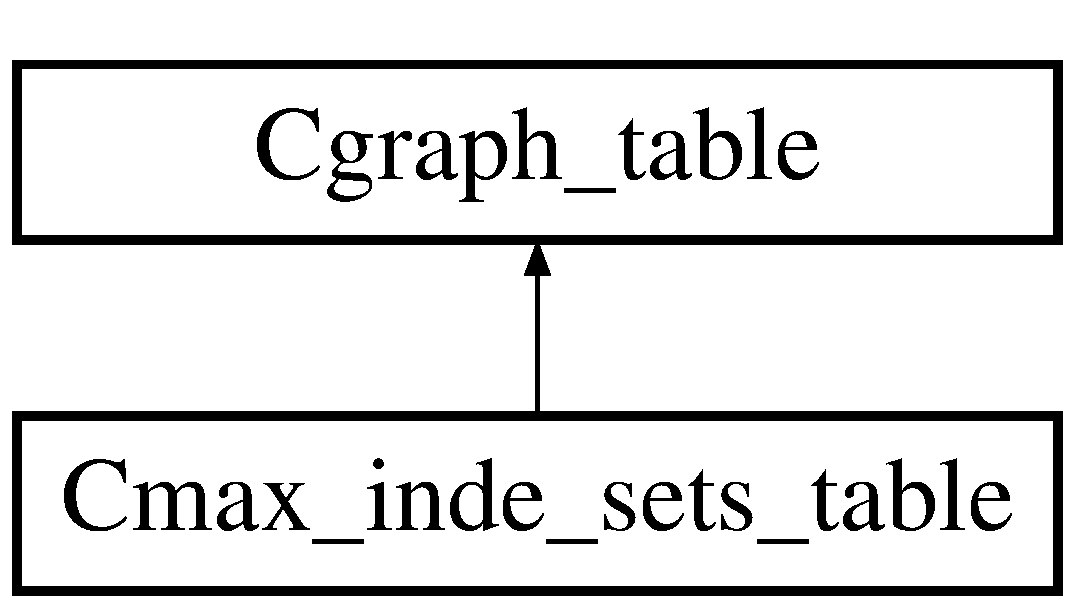
\includegraphics[height=2.000000cm]{class_cgraph__table}
\end{center}
\end{figure}
\subsection*{Public Member Functions}
\begin{DoxyCompactItemize}
\item 
\hyperlink{class_cgraph__table_aabb74d501db61369797903de6329fe87}{Cgraph\+\_\+table} ()
\begin{DoxyCompactList}\small\item\em Purpose\+: create a new \hyperlink{class_cgraph__table}{Cgraph\+\_\+table} with null value. \end{DoxyCompactList}\item 
\hyperlink{class_cgraph__table_a3449715030a5e9365b35554ad75d3919}{Cgraph\+\_\+table} (const \hyperlink{class_cgraph__table}{Cgraph\+\_\+table} \&Cgraph\+\_\+table\+\_\+to\+\_\+copy)
\begin{DoxyCompactList}\small\item\em Purpose\+: create a new \hyperlink{class_cgraph__table}{Cgraph\+\_\+table} with the value of the one in parameter. \end{DoxyCompactList}\item 
\hyperlink{class_cgraph__table_a8a3d1269cabe8a29d1b6e004e1a88a1b}{$\sim$\+Cgraph\+\_\+table} ()
\begin{DoxyCompactList}\small\item\em Purpose\+: delete correctly a \hyperlink{class_cgraph__table}{Cgraph\+\_\+table}. \end{DoxyCompactList}\item 
void \hyperlink{class_cgraph__table_a6ac26aa9fbc81ea02cfec30a2062c4e3}{G\+R\+Tempty\+\_\+table} ()
\begin{DoxyCompactList}\small\item\em Purpose\+: remove all the Graph in the \hyperlink{class_cgraph__table}{Cgraph\+\_\+table}. \end{DoxyCompactList}\item 
\hyperlink{class_cgraph}{Cgraph} $\ast$$\ast$ \hyperlink{class_cgraph__table_a2a00e51699671b8fc9788729b6ee8d51}{G\+R\+Tget\+\_\+graph\+\_\+table} ()
\begin{DoxyCompactList}\small\item\em Purpose\+: get the table of graph. \end{DoxyCompactList}\item 
\hyperlink{class_cgraph}{Cgraph} $\ast$ \hyperlink{class_cgraph__table_a9ad5111e2f01f7b18b289a828007d100}{G\+R\+Tget\+\_\+graph} (unsigned int ui\+Index)
\begin{DoxyCompactList}\small\item\em Purpose\+: get the graph at the index in the table. \end{DoxyCompactList}\item 
unsigned int \hyperlink{class_cgraph__table_a402ccf4db0c95c9aa0a2220734c3386f}{G\+R\+Tget\+\_\+nb\+\_\+graph} ()
\begin{DoxyCompactList}\small\item\em Purpose\+: get the number of graph in the table. \end{DoxyCompactList}\item 
void \hyperlink{class_cgraph__table_aa2c4e7d9a6c2ec7c555d5f325208fc99}{G\+R\+Tadd\+\_\+graph} (\hyperlink{class_cgraph}{Cgraph} $\ast$p\+Graph)
\begin{DoxyCompactList}\small\item\em Purpose\+: add a graph to the table. \end{DoxyCompactList}\item 
\hyperlink{class_cgraph}{Cgraph} $\ast$ \hyperlink{class_cgraph__table_a441f71c44ac878bcac4af61f7a096155}{G\+R\+T\+\_\+delete\+\_\+graph\+\_\+at\+\_\+index} (unsigned int ui\+Index)
\begin{DoxyCompactList}\small\item\em Purpose\+: delete a graph at the specified position. \end{DoxyCompactList}\item 
void \hyperlink{class_cgraph__table_a047848af6b236a03c66da886a0a35d05}{G\+R\+T\+\_\+insert\+\_\+graph\+\_\+at\+\_\+index} (unsigned int ui\+Index, \hyperlink{class_cgraph}{Cgraph} $\ast$p\+Cgraph\+\_\+to\+\_\+add)
\begin{DoxyCompactList}\small\item\em Purpose\+: insert a graph at the position in parameter. \end{DoxyCompactList}\item 
\hyperlink{class_cgraph}{Cgraph} $\ast$ \hyperlink{class_cgraph__table_af6e3a18e66cff9421ee94e08e77bb30c}{G\+R\+T\+\_\+replace\+\_\+graph\+\_\+at\+\_\+index} (unsigned int ui\+Index, \hyperlink{class_cgraph}{Cgraph} $\ast$p\+Cgraph\+\_\+to\+\_\+add)
\begin{DoxyCompactList}\small\item\em Purpose\+: replace the graph at the index by the one in parameter. \end{DoxyCompactList}\item 
void \hyperlink{class_cgraph__table_a3710eca1f83462c7e297856cfdf4704b}{G\+R\+Tprint} ()
\begin{DoxyCompactList}\small\item\em Purpose\+: print the independant sets. \end{DoxyCompactList}\item 
\hyperlink{class_cgraph__table}{Cgraph\+\_\+table} \& \hyperlink{class_cgraph__table_adf1965acc4d5d0b355eb4b86e375223f}{operator=} (const \hyperlink{class_cgraph__table}{Cgraph\+\_\+table} \&graph\+\_\+table\+\_\+to\+\_\+copy)
\begin{DoxyCompactList}\small\item\em Purpose\+: set the value of a graph table with equal operator. \end{DoxyCompactList}\item 
bool \hyperlink{class_cgraph__table_a6a85919582df0a578740405744072229}{operator==} (\hyperlink{class_cgraph__table}{Cgraph\+\_\+table} \&graph\+\_\+table\+\_\+to\+\_\+compare) const 
\begin{DoxyCompactList}\small\item\em Purpose\+: compare two graph table. \end{DoxyCompactList}\item 
bool \hyperlink{class_cgraph__table_aaaeda8063b2da6052a7a3c482337d793}{operator!=} (\hyperlink{class_cgraph__table}{Cgraph\+\_\+table} \&graph\+\_\+table\+\_\+to\+\_\+compare) const 
\begin{DoxyCompactList}\small\item\em Purpose\+: compare two graph table. \end{DoxyCompactList}\end{DoxyCompactItemize}
\subsection*{Private Attributes}
\begin{DoxyCompactItemize}
\item 
\hyperlink{class_cgraph}{Cgraph} $\ast$$\ast$ \hyperlink{class_cgraph__table_a0aa721f87c50e553fe2d7ff8a23d1673}{pp\+G\+R\+Tgraph\+\_\+table}
\item 
unsigned int \hyperlink{class_cgraph__table_a87fbe4f547d5fa7b94697ba7b1fedc66}{ui\+G\+R\+Tnb\+\_\+graph}
\end{DoxyCompactItemize}


\subsection{Detailed Description}
\hyperlink{class_cgraph__table}{Cgraph\+\_\+table} Class. 

Definition at line 14 of file Cgraph\+\_\+table.\+h.



\subsection{Constructor \& Destructor Documentation}
\hypertarget{class_cgraph__table_aabb74d501db61369797903de6329fe87}{}\index{Cgraph\+\_\+table@{Cgraph\+\_\+table}!Cgraph\+\_\+table@{Cgraph\+\_\+table}}
\index{Cgraph\+\_\+table@{Cgraph\+\_\+table}!Cgraph\+\_\+table@{Cgraph\+\_\+table}}
\subsubsection[{Cgraph\+\_\+table}]{\setlength{\rightskip}{0pt plus 5cm}Cgraph\+\_\+table\+::\+Cgraph\+\_\+table (
\begin{DoxyParamCaption}
{}
\end{DoxyParamCaption}
)}\label{class_cgraph__table_aabb74d501db61369797903de6329fe87}


Purpose\+: create a new \hyperlink{class_cgraph__table}{Cgraph\+\_\+table} with null value. 

\hyperlink{class_cgraph__table_aabb74d501db61369797903de6329fe87}{Cgraph\+\_\+table()} -\/ create a new \hyperlink{class_cgraph__table}{Cgraph\+\_\+table} with null value


\begin{DoxyParams}{Parameters}
{\em none} & \\
\hline
\end{DoxyParams}
\begin{DoxyReturn}{Returns}
none 
\end{DoxyReturn}


Definition at line 16 of file Cgraph\+\_\+table.\+cpp.

\hypertarget{class_cgraph__table_a3449715030a5e9365b35554ad75d3919}{}\index{Cgraph\+\_\+table@{Cgraph\+\_\+table}!Cgraph\+\_\+table@{Cgraph\+\_\+table}}
\index{Cgraph\+\_\+table@{Cgraph\+\_\+table}!Cgraph\+\_\+table@{Cgraph\+\_\+table}}
\subsubsection[{Cgraph\+\_\+table}]{\setlength{\rightskip}{0pt plus 5cm}Cgraph\+\_\+table\+::\+Cgraph\+\_\+table (
\begin{DoxyParamCaption}
\item[{const {\bf Cgraph\+\_\+table} \&}]{Cgraph\+\_\+table\+\_\+to\+\_\+copy}
\end{DoxyParamCaption}
)}\label{class_cgraph__table_a3449715030a5e9365b35554ad75d3919}


Purpose\+: create a new \hyperlink{class_cgraph__table}{Cgraph\+\_\+table} with the value of the one in parameter. 

\hyperlink{class_cgraph__table_a3449715030a5e9365b35554ad75d3919}{Cgraph\+\_\+table(const Cgraph\+\_\+table \& Cgraph\+\_\+table\+\_\+to\+\_\+copy)} -\/ create a new \hyperlink{class_cgraph__table}{Cgraph\+\_\+table} with the value of the one in parameter


\begin{DoxyParams}{Parameters}
{\em const} & \hyperlink{class_cgraph__table}{Cgraph\+\_\+table} \& Cgraph\+\_\+table\+\_\+to\+\_\+copy -\/ the graph to copy\\
\hline
\end{DoxyParams}
\begin{DoxyReturn}{Returns}
none 
\end{DoxyReturn}


Definition at line 35 of file Cgraph\+\_\+table.\+cpp.

\hypertarget{class_cgraph__table_a8a3d1269cabe8a29d1b6e004e1a88a1b}{}\index{Cgraph\+\_\+table@{Cgraph\+\_\+table}!````~Cgraph\+\_\+table@{$\sim$\+Cgraph\+\_\+table}}
\index{````~Cgraph\+\_\+table@{$\sim$\+Cgraph\+\_\+table}!Cgraph\+\_\+table@{Cgraph\+\_\+table}}
\subsubsection[{$\sim$\+Cgraph\+\_\+table}]{\setlength{\rightskip}{0pt plus 5cm}Cgraph\+\_\+table\+::$\sim$\+Cgraph\+\_\+table (
\begin{DoxyParamCaption}
{}
\end{DoxyParamCaption}
)}\label{class_cgraph__table_a8a3d1269cabe8a29d1b6e004e1a88a1b}


Purpose\+: delete correctly a \hyperlink{class_cgraph__table}{Cgraph\+\_\+table}. 

\hyperlink{class_cgraph__table_a8a3d1269cabe8a29d1b6e004e1a88a1b}{$\sim$\+Cgraph\+\_\+table()} -\/ delete correctly a \hyperlink{class_cgraph__table}{Cgraph\+\_\+table}


\begin{DoxyParams}{Parameters}
{\em none} & \\
\hline
\end{DoxyParams}
\begin{DoxyReturn}{Returns}
none 
\end{DoxyReturn}


Definition at line 57 of file Cgraph\+\_\+table.\+cpp.



\subsection{Member Function Documentation}
\hypertarget{class_cgraph__table_a441f71c44ac878bcac4af61f7a096155}{}\index{Cgraph\+\_\+table@{Cgraph\+\_\+table}!G\+R\+T\+\_\+delete\+\_\+graph\+\_\+at\+\_\+index@{G\+R\+T\+\_\+delete\+\_\+graph\+\_\+at\+\_\+index}}
\index{G\+R\+T\+\_\+delete\+\_\+graph\+\_\+at\+\_\+index@{G\+R\+T\+\_\+delete\+\_\+graph\+\_\+at\+\_\+index}!Cgraph\+\_\+table@{Cgraph\+\_\+table}}
\subsubsection[{G\+R\+T\+\_\+delete\+\_\+graph\+\_\+at\+\_\+index}]{\setlength{\rightskip}{0pt plus 5cm}{\bf Cgraph} $\ast$ Cgraph\+\_\+table\+::\+G\+R\+T\+\_\+delete\+\_\+graph\+\_\+at\+\_\+index (
\begin{DoxyParamCaption}
\item[{unsigned int}]{ui\+Index}
\end{DoxyParamCaption}
)}\label{class_cgraph__table_a441f71c44ac878bcac4af61f7a096155}


Purpose\+: delete a graph at the specified position. 

\hyperlink{class_cgraph}{Cgraph} $\ast$ \hyperlink{class_cgraph__table_a441f71c44ac878bcac4af61f7a096155}{Cgraph\+\_\+table\+::\+G\+R\+T\+\_\+delete\+\_\+graph\+\_\+at\+\_\+index(unsigned int ui\+Index)} -\/ delete a graph at the specified position


\begin{DoxyParams}{Parameters}
{\em unsigned} & int ui\+Index -\/ index of the graph to be removed\\
\hline
\end{DoxyParams}
\begin{DoxyReturn}{Returns}
\hyperlink{class_cgraph}{Cgraph} $\ast$ -\/ the graph who will be removed
\end{DoxyReturn}

\begin{DoxyExceptions}{Exceptions}
{\em Throw} & an exception if index is outofbound \\
\hline
\end{DoxyExceptions}


Definition at line 191 of file Cgraph\+\_\+table.\+cpp.

\hypertarget{class_cgraph__table_a047848af6b236a03c66da886a0a35d05}{}\index{Cgraph\+\_\+table@{Cgraph\+\_\+table}!G\+R\+T\+\_\+insert\+\_\+graph\+\_\+at\+\_\+index@{G\+R\+T\+\_\+insert\+\_\+graph\+\_\+at\+\_\+index}}
\index{G\+R\+T\+\_\+insert\+\_\+graph\+\_\+at\+\_\+index@{G\+R\+T\+\_\+insert\+\_\+graph\+\_\+at\+\_\+index}!Cgraph\+\_\+table@{Cgraph\+\_\+table}}
\subsubsection[{G\+R\+T\+\_\+insert\+\_\+graph\+\_\+at\+\_\+index}]{\setlength{\rightskip}{0pt plus 5cm}void Cgraph\+\_\+table\+::\+G\+R\+T\+\_\+insert\+\_\+graph\+\_\+at\+\_\+index (
\begin{DoxyParamCaption}
\item[{unsigned int}]{ui\+Index, }
\item[{{\bf Cgraph} $\ast$}]{p\+Cgraph\+\_\+to\+\_\+add}
\end{DoxyParamCaption}
)}\label{class_cgraph__table_a047848af6b236a03c66da886a0a35d05}


Purpose\+: insert a graph at the position in parameter. 

void \hyperlink{class_cgraph__table_a047848af6b236a03c66da886a0a35d05}{Cgraph\+\_\+table\+::\+G\+R\+T\+\_\+insert\+\_\+graph\+\_\+at\+\_\+index(unsigned int ui\+Index, Cgraph $\ast$ p\+Cgraph\+\_\+to\+\_\+add)} -\/ insert a graph at the position in parameter


\begin{DoxyParams}{Parameters}
{\em unsigned} & int ui\+Index -\/ index of the graph to be inserted \hyperlink{class_cgraph}{Cgraph} $\ast$ p\+Graph -\/ graph to set\\
\hline
\end{DoxyParams}
\begin{DoxyReturn}{Returns}
\hyperlink{class_cgraph}{Cgraph} $\ast$ -\/ the graph who will be removed
\end{DoxyReturn}

\begin{DoxyExceptions}{Exceptions}
{\em Throw} & an exception if index is outofbound \\
\hline
\end{DoxyExceptions}


Definition at line 244 of file Cgraph\+\_\+table.\+cpp.

\hypertarget{class_cgraph__table_af6e3a18e66cff9421ee94e08e77bb30c}{}\index{Cgraph\+\_\+table@{Cgraph\+\_\+table}!G\+R\+T\+\_\+replace\+\_\+graph\+\_\+at\+\_\+index@{G\+R\+T\+\_\+replace\+\_\+graph\+\_\+at\+\_\+index}}
\index{G\+R\+T\+\_\+replace\+\_\+graph\+\_\+at\+\_\+index@{G\+R\+T\+\_\+replace\+\_\+graph\+\_\+at\+\_\+index}!Cgraph\+\_\+table@{Cgraph\+\_\+table}}
\subsubsection[{G\+R\+T\+\_\+replace\+\_\+graph\+\_\+at\+\_\+index}]{\setlength{\rightskip}{0pt plus 5cm}{\bf Cgraph} $\ast$ Cgraph\+\_\+table\+::\+G\+R\+T\+\_\+replace\+\_\+graph\+\_\+at\+\_\+index (
\begin{DoxyParamCaption}
\item[{unsigned int}]{ui\+Index, }
\item[{{\bf Cgraph} $\ast$}]{p\+Cgraph\+\_\+to\+\_\+add}
\end{DoxyParamCaption}
)}\label{class_cgraph__table_af6e3a18e66cff9421ee94e08e77bb30c}


Purpose\+: replace the graph at the index by the one in parameter. 

\hyperlink{class_cgraph}{Cgraph} $\ast$ \hyperlink{class_cgraph__table_af6e3a18e66cff9421ee94e08e77bb30c}{Cgraph\+\_\+table\+::\+G\+R\+T\+\_\+replace\+\_\+graph\+\_\+at\+\_\+index(unsigned int ui\+Index, Cgraph $\ast$ p\+Graph)} -\/ replace the graph at the index by the one in parameter


\begin{DoxyParams}{Parameters}
{\em unsigned} & int ui\+Index -\/ index of the graph to be replaced \hyperlink{class_cgraph}{Cgraph} $\ast$ p\+Graph -\/ graph to set\\
\hline
\end{DoxyParams}
\begin{DoxyReturn}{Returns}
\hyperlink{class_cgraph}{Cgraph} $\ast$ -\/ the graph who will be removed, null if the index is outofbound 
\end{DoxyReturn}


Definition at line 295 of file Cgraph\+\_\+table.\+cpp.

\hypertarget{class_cgraph__table_aa2c4e7d9a6c2ec7c555d5f325208fc99}{}\index{Cgraph\+\_\+table@{Cgraph\+\_\+table}!G\+R\+Tadd\+\_\+graph@{G\+R\+Tadd\+\_\+graph}}
\index{G\+R\+Tadd\+\_\+graph@{G\+R\+Tadd\+\_\+graph}!Cgraph\+\_\+table@{Cgraph\+\_\+table}}
\subsubsection[{G\+R\+Tadd\+\_\+graph}]{\setlength{\rightskip}{0pt plus 5cm}void Cgraph\+\_\+table\+::\+G\+R\+Tadd\+\_\+graph (
\begin{DoxyParamCaption}
\item[{{\bf Cgraph} $\ast$}]{p\+Graph}
\end{DoxyParamCaption}
)}\label{class_cgraph__table_aa2c4e7d9a6c2ec7c555d5f325208fc99}


Purpose\+: add a graph to the table. 

void \hyperlink{class_cgraph__table_aa2c4e7d9a6c2ec7c555d5f325208fc99}{G\+R\+Tadd\+\_\+graph(\+Cgraph $\ast$ p\+Graph)} -\/ add a graph to the table


\begin{DoxyParams}{Parameters}
{\em \hyperlink{class_cgraph}{Cgraph}} & $\ast$ p\+Graph -\/ the graph to add\\
\hline
\end{DoxyParams}
\begin{DoxyReturn}{Returns}
none 
\end{DoxyReturn}


Definition at line 157 of file Cgraph\+\_\+table.\+cpp.

\hypertarget{class_cgraph__table_a6ac26aa9fbc81ea02cfec30a2062c4e3}{}\index{Cgraph\+\_\+table@{Cgraph\+\_\+table}!G\+R\+Tempty\+\_\+table@{G\+R\+Tempty\+\_\+table}}
\index{G\+R\+Tempty\+\_\+table@{G\+R\+Tempty\+\_\+table}!Cgraph\+\_\+table@{Cgraph\+\_\+table}}
\subsubsection[{G\+R\+Tempty\+\_\+table}]{\setlength{\rightskip}{0pt plus 5cm}void Cgraph\+\_\+table\+::\+G\+R\+Tempty\+\_\+table (
\begin{DoxyParamCaption}
{}
\end{DoxyParamCaption}
)}\label{class_cgraph__table_a6ac26aa9fbc81ea02cfec30a2062c4e3}


Purpose\+: remove all the Graph in the \hyperlink{class_cgraph__table}{Cgraph\+\_\+table}. 

void \hyperlink{class_cgraph__table_a6ac26aa9fbc81ea02cfec30a2062c4e3}{G\+R\+Tempty\+\_\+table()} -\/ remove all the Graph in the \hyperlink{class_cgraph__table}{Cgraph\+\_\+table}


\begin{DoxyParams}{Parameters}
{\em none} & \\
\hline
\end{DoxyParams}
\begin{DoxyReturn}{Returns}
none 
\end{DoxyReturn}


Definition at line 74 of file Cgraph\+\_\+table.\+cpp.

\hypertarget{class_cgraph__table_a9ad5111e2f01f7b18b289a828007d100}{}\index{Cgraph\+\_\+table@{Cgraph\+\_\+table}!G\+R\+Tget\+\_\+graph@{G\+R\+Tget\+\_\+graph}}
\index{G\+R\+Tget\+\_\+graph@{G\+R\+Tget\+\_\+graph}!Cgraph\+\_\+table@{Cgraph\+\_\+table}}
\subsubsection[{G\+R\+Tget\+\_\+graph}]{\setlength{\rightskip}{0pt plus 5cm}{\bf Cgraph} $\ast$ Cgraph\+\_\+table\+::\+G\+R\+Tget\+\_\+graph (
\begin{DoxyParamCaption}
\item[{unsigned int}]{ui\+Index}
\end{DoxyParamCaption}
)}\label{class_cgraph__table_a9ad5111e2f01f7b18b289a828007d100}


Purpose\+: get the graph at the index in the table. 

\hyperlink{class_cgraph}{Cgraph} $\ast$ \hyperlink{class_cgraph__table_a9ad5111e2f01f7b18b289a828007d100}{G\+R\+Tget\+\_\+graph(unsigned int ui\+Index)} -\/ get the graph at the index


\begin{DoxyParams}{Parameters}
{\em none} & \\
\hline
\end{DoxyParams}
\begin{DoxyReturn}{Returns}
none 
\end{DoxyReturn}


Definition at line 117 of file Cgraph\+\_\+table.\+cpp.

\hypertarget{class_cgraph__table_a2a00e51699671b8fc9788729b6ee8d51}{}\index{Cgraph\+\_\+table@{Cgraph\+\_\+table}!G\+R\+Tget\+\_\+graph\+\_\+table@{G\+R\+Tget\+\_\+graph\+\_\+table}}
\index{G\+R\+Tget\+\_\+graph\+\_\+table@{G\+R\+Tget\+\_\+graph\+\_\+table}!Cgraph\+\_\+table@{Cgraph\+\_\+table}}
\subsubsection[{G\+R\+Tget\+\_\+graph\+\_\+table}]{\setlength{\rightskip}{0pt plus 5cm}{\bf Cgraph} $\ast$$\ast$ Cgraph\+\_\+table\+::\+G\+R\+Tget\+\_\+graph\+\_\+table (
\begin{DoxyParamCaption}
{}
\end{DoxyParamCaption}
)}\label{class_cgraph__table_a2a00e51699671b8fc9788729b6ee8d51}


Purpose\+: get the table of graph. 

\hyperlink{class_cgraph}{Cgraph} $\ast$ \hyperlink{class_cgraph__table_a2a00e51699671b8fc9788729b6ee8d51}{G\+R\+Tget\+\_\+graph\+\_\+table()} -\/ get the table of graph at the index


\begin{DoxyParams}{Parameters}
{\em none} & \\
\hline
\end{DoxyParams}
\begin{DoxyReturn}{Returns}
none 
\end{DoxyReturn}


Definition at line 100 of file Cgraph\+\_\+table.\+cpp.

\hypertarget{class_cgraph__table_a402ccf4db0c95c9aa0a2220734c3386f}{}\index{Cgraph\+\_\+table@{Cgraph\+\_\+table}!G\+R\+Tget\+\_\+nb\+\_\+graph@{G\+R\+Tget\+\_\+nb\+\_\+graph}}
\index{G\+R\+Tget\+\_\+nb\+\_\+graph@{G\+R\+Tget\+\_\+nb\+\_\+graph}!Cgraph\+\_\+table@{Cgraph\+\_\+table}}
\subsubsection[{G\+R\+Tget\+\_\+nb\+\_\+graph}]{\setlength{\rightskip}{0pt plus 5cm}unsigned int Cgraph\+\_\+table\+::\+G\+R\+Tget\+\_\+nb\+\_\+graph (
\begin{DoxyParamCaption}
{}
\end{DoxyParamCaption}
)}\label{class_cgraph__table_a402ccf4db0c95c9aa0a2220734c3386f}


Purpose\+: get the number of graph in the table. 

unsigned int \hyperlink{class_cgraph__table_a402ccf4db0c95c9aa0a2220734c3386f}{G\+R\+Tget\+\_\+nb\+\_\+graph()} -\/ get the number of graph in the table


\begin{DoxyParams}{Parameters}
{\em unsigned} & int ui\+Index -\/ the index of the graph to get\\
\hline
\end{DoxyParams}
\begin{DoxyReturn}{Returns}
unsigned int -\/ the number of graph 
\end{DoxyReturn}


Definition at line 140 of file Cgraph\+\_\+table.\+cpp.

\hypertarget{class_cgraph__table_a3710eca1f83462c7e297856cfdf4704b}{}\index{Cgraph\+\_\+table@{Cgraph\+\_\+table}!G\+R\+Tprint@{G\+R\+Tprint}}
\index{G\+R\+Tprint@{G\+R\+Tprint}!Cgraph\+\_\+table@{Cgraph\+\_\+table}}
\subsubsection[{G\+R\+Tprint}]{\setlength{\rightskip}{0pt plus 5cm}void Cgraph\+\_\+table\+::\+G\+R\+Tprint (
\begin{DoxyParamCaption}
{}
\end{DoxyParamCaption}
)}\label{class_cgraph__table_a3710eca1f83462c7e297856cfdf4704b}


Purpose\+: print the independant sets. 

void \hyperlink{class_cgraph__table_a3710eca1f83462c7e297856cfdf4704b}{G\+R\+Tprint()} -\/ print the independant sets


\begin{DoxyParams}{Parameters}
{\em none} & \\
\hline
\end{DoxyParams}
\begin{DoxyReturn}{Returns}
none 
\end{DoxyReturn}


Definition at line 320 of file Cgraph\+\_\+table.\+cpp.

\hypertarget{class_cgraph__table_aaaeda8063b2da6052a7a3c482337d793}{}\index{Cgraph\+\_\+table@{Cgraph\+\_\+table}!operator"!=@{operator"!=}}
\index{operator"!=@{operator"!=}!Cgraph\+\_\+table@{Cgraph\+\_\+table}}
\subsubsection[{operator"!=}]{\setlength{\rightskip}{0pt plus 5cm}bool Cgraph\+\_\+table\+::operator!= (
\begin{DoxyParamCaption}
\item[{{\bf Cgraph\+\_\+table} \&}]{graph\+\_\+table\+\_\+to\+\_\+compare}
\end{DoxyParamCaption}
) const}\label{class_cgraph__table_aaaeda8063b2da6052a7a3c482337d793}


Purpose\+: compare two graph table. 

bool Cgraph\+\_\+table\+::operator!=(\+Cgraph \&graph\+To\+Compare)const -\/ compare two graph table


\begin{DoxyParams}{Parameters}
{\em \hyperlink{class_cgraph__table}{Cgraph\+\_\+table}} & \& graph\+\_\+table\+\_\+to\+\_\+compare -\/ the graph table to compare\\
\hline
\end{DoxyParams}
\begin{DoxyReturn}{Returns}
true -\/ if the two graph\+\_\+table are different 
\end{DoxyReturn}


Definition at line 413 of file Cgraph\+\_\+table.\+cpp.

\hypertarget{class_cgraph__table_adf1965acc4d5d0b355eb4b86e375223f}{}\index{Cgraph\+\_\+table@{Cgraph\+\_\+table}!operator=@{operator=}}
\index{operator=@{operator=}!Cgraph\+\_\+table@{Cgraph\+\_\+table}}
\subsubsection[{operator=}]{\setlength{\rightskip}{0pt plus 5cm}{\bf Cgraph\+\_\+table} \& Cgraph\+\_\+table\+::operator= (
\begin{DoxyParamCaption}
\item[{const {\bf Cgraph\+\_\+table} \&}]{graph\+\_\+table\+\_\+to\+\_\+copy}
\end{DoxyParamCaption}
)}\label{class_cgraph__table_adf1965acc4d5d0b355eb4b86e375223f}


Purpose\+: set the value of a graph table with equal operator. 

\hyperlink{class_cgraph}{Cgraph} \& Cgraph\+\_\+table\+::operator=(const Cgraph \&graph\+\_\+to\+\_\+copy) -\/ set the value of a graph table with equal operator


\begin{DoxyParams}{Parameters}
{\em const} & \hyperlink{class_cgraph}{Cgraph} \& graph\+\_\+table\+\_\+to\+\_\+copy -\/ the graph table to copy (use to set the value)\\
\hline
\end{DoxyParams}
\begin{DoxyReturn}{Returns}
none 
\end{DoxyReturn}


Definition at line 341 of file Cgraph\+\_\+table.\+cpp.

\hypertarget{class_cgraph__table_a6a85919582df0a578740405744072229}{}\index{Cgraph\+\_\+table@{Cgraph\+\_\+table}!operator==@{operator==}}
\index{operator==@{operator==}!Cgraph\+\_\+table@{Cgraph\+\_\+table}}
\subsubsection[{operator==}]{\setlength{\rightskip}{0pt plus 5cm}bool Cgraph\+\_\+table\+::operator== (
\begin{DoxyParamCaption}
\item[{{\bf Cgraph\+\_\+table} \&}]{graph\+\_\+table\+\_\+to\+\_\+compare}
\end{DoxyParamCaption}
) const}\label{class_cgraph__table_a6a85919582df0a578740405744072229}


Purpose\+: compare two graph table. 

bool Cgraph\+\_\+table\+::operator==(\+Cgraph \&graph\+To\+Compare)const -\/ compare two graph table


\begin{DoxyParams}{Parameters}
{\em \hyperlink{class_cgraph__table}{Cgraph\+\_\+table}} & \& graph\+\_\+table\+\_\+to\+\_\+compare -\/ the graph table to compare\\
\hline
\end{DoxyParams}
\begin{DoxyReturn}{Returns}
true -\/ if the two graphe\+\_\+table are equal 
\end{DoxyReturn}


Definition at line 370 of file Cgraph\+\_\+table.\+cpp.



\subsection{Member Data Documentation}
\hypertarget{class_cgraph__table_a0aa721f87c50e553fe2d7ff8a23d1673}{}\index{Cgraph\+\_\+table@{Cgraph\+\_\+table}!pp\+G\+R\+Tgraph\+\_\+table@{pp\+G\+R\+Tgraph\+\_\+table}}
\index{pp\+G\+R\+Tgraph\+\_\+table@{pp\+G\+R\+Tgraph\+\_\+table}!Cgraph\+\_\+table@{Cgraph\+\_\+table}}
\subsubsection[{pp\+G\+R\+Tgraph\+\_\+table}]{\setlength{\rightskip}{0pt plus 5cm}{\bf Cgraph}$\ast$$\ast$ Cgraph\+\_\+table\+::pp\+G\+R\+Tgraph\+\_\+table\hspace{0.3cm}{\ttfamily [private]}}\label{class_cgraph__table_a0aa721f87c50e553fe2d7ff8a23d1673}


Definition at line 18 of file Cgraph\+\_\+table.\+h.

\hypertarget{class_cgraph__table_a87fbe4f547d5fa7b94697ba7b1fedc66}{}\index{Cgraph\+\_\+table@{Cgraph\+\_\+table}!ui\+G\+R\+Tnb\+\_\+graph@{ui\+G\+R\+Tnb\+\_\+graph}}
\index{ui\+G\+R\+Tnb\+\_\+graph@{ui\+G\+R\+Tnb\+\_\+graph}!Cgraph\+\_\+table@{Cgraph\+\_\+table}}
\subsubsection[{ui\+G\+R\+Tnb\+\_\+graph}]{\setlength{\rightskip}{0pt plus 5cm}unsigned int Cgraph\+\_\+table\+::ui\+G\+R\+Tnb\+\_\+graph\hspace{0.3cm}{\ttfamily [private]}}\label{class_cgraph__table_a87fbe4f547d5fa7b94697ba7b1fedc66}


Definition at line 19 of file Cgraph\+\_\+table.\+h.



The documentation for this class was generated from the following files\+:\begin{DoxyCompactItemize}
\item 
Projet\+Cpp-\/\+Stable/\hyperlink{_cgraph__table_8h}{Cgraph\+\_\+table.\+h}\item 
Projet\+Cpp-\/\+Stable/\hyperlink{_cgraph__table_8cpp}{Cgraph\+\_\+table.\+cpp}\end{DoxyCompactItemize}

\hypertarget{class_cgraph__table___u_n_i_t}{}\section{Cgraph\+\_\+table\+\_\+\+U\+N\+I\+T Class Reference}
\label{class_cgraph__table___u_n_i_t}\index{Cgraph\+\_\+table\+\_\+\+U\+N\+I\+T@{Cgraph\+\_\+table\+\_\+\+U\+N\+I\+T}}


\hyperlink{class_cgraph__table___u_n_i_t}{Cgraph\+\_\+table\+\_\+\+U\+N\+I\+T} Class.  




{\ttfamily \#include $<$Cgraph\+\_\+table\+\_\+\+U\+N\+I\+T.\+h$>$}

\subsection*{Static Public Member Functions}
\begin{DoxyCompactItemize}
\item 
static void \hyperlink{class_cgraph__table___u_n_i_t_a04573717abf01682c609eea51388ec40}{T\+E\+S\+T\+\_\+\+U\+N\+I\+T\+\_\+\+Cgraph\+\_\+table} ()
\item 
static void \hyperlink{class_cgraph__table___u_n_i_t_a0adeae0b1160e3289d707a6cfc160b7c}{T\+E\+S\+T\+\_\+\+U\+N\+I\+T\+\_\+\+G\+R\+Tempty\+\_\+table} ()
\item 
static void \hyperlink{class_cgraph__table___u_n_i_t_a4e060c1a29a7a9e26cc005ea94049e89}{T\+E\+S\+T\+\_\+\+U\+N\+I\+T\+\_\+\+G\+R\+T\+\_\+delete\+\_\+graph\+\_\+at\+\_\+index} ()
\item 
static void \hyperlink{class_cgraph__table___u_n_i_t_a89a7696c6851df4d449842e585bd936c}{T\+E\+S\+T\+\_\+\+U\+N\+I\+T\+\_\+\+G\+R\+T\+\_\+insert\+\_\+graph\+\_\+at\+\_\+index} ()
\item 
static void \hyperlink{class_cgraph__table___u_n_i_t_ab3ddda590372f2992112626466e0514f}{T\+E\+S\+T\+\_\+\+U\+N\+I\+T\+\_\+\+G\+R\+T\+\_\+replace\+\_\+graph\+\_\+at\+\_\+index} ()
\end{DoxyCompactItemize}


\subsection{Detailed Description}
\hyperlink{class_cgraph__table___u_n_i_t}{Cgraph\+\_\+table\+\_\+\+U\+N\+I\+T} Class. 

Definition at line 13 of file Cgraph\+\_\+table\+\_\+\+U\+N\+I\+T.\+h.



\subsection{Member Function Documentation}
\hypertarget{class_cgraph__table___u_n_i_t_a04573717abf01682c609eea51388ec40}{}\index{Cgraph\+\_\+table\+\_\+\+U\+N\+I\+T@{Cgraph\+\_\+table\+\_\+\+U\+N\+I\+T}!T\+E\+S\+T\+\_\+\+U\+N\+I\+T\+\_\+\+Cgraph\+\_\+table@{T\+E\+S\+T\+\_\+\+U\+N\+I\+T\+\_\+\+Cgraph\+\_\+table}}
\index{T\+E\+S\+T\+\_\+\+U\+N\+I\+T\+\_\+\+Cgraph\+\_\+table@{T\+E\+S\+T\+\_\+\+U\+N\+I\+T\+\_\+\+Cgraph\+\_\+table}!Cgraph\+\_\+table\+\_\+\+U\+N\+I\+T@{Cgraph\+\_\+table\+\_\+\+U\+N\+I\+T}}
\subsubsection[{T\+E\+S\+T\+\_\+\+U\+N\+I\+T\+\_\+\+Cgraph\+\_\+table}]{\setlength{\rightskip}{0pt plus 5cm}void Cgraph\+\_\+table\+\_\+\+U\+N\+I\+T\+::\+T\+E\+S\+T\+\_\+\+U\+N\+I\+T\+\_\+\+Cgraph\+\_\+table (
\begin{DoxyParamCaption}
{}
\end{DoxyParamCaption}
)\hspace{0.3cm}{\ttfamily [static]}}\label{class_cgraph__table___u_n_i_t_a04573717abf01682c609eea51388ec40}


Definition at line 5 of file Cgraph\+\_\+table\+\_\+\+U\+N\+I\+T.\+cpp.

\hypertarget{class_cgraph__table___u_n_i_t_a4e060c1a29a7a9e26cc005ea94049e89}{}\index{Cgraph\+\_\+table\+\_\+\+U\+N\+I\+T@{Cgraph\+\_\+table\+\_\+\+U\+N\+I\+T}!T\+E\+S\+T\+\_\+\+U\+N\+I\+T\+\_\+\+G\+R\+T\+\_\+delete\+\_\+graph\+\_\+at\+\_\+index@{T\+E\+S\+T\+\_\+\+U\+N\+I\+T\+\_\+\+G\+R\+T\+\_\+delete\+\_\+graph\+\_\+at\+\_\+index}}
\index{T\+E\+S\+T\+\_\+\+U\+N\+I\+T\+\_\+\+G\+R\+T\+\_\+delete\+\_\+graph\+\_\+at\+\_\+index@{T\+E\+S\+T\+\_\+\+U\+N\+I\+T\+\_\+\+G\+R\+T\+\_\+delete\+\_\+graph\+\_\+at\+\_\+index}!Cgraph\+\_\+table\+\_\+\+U\+N\+I\+T@{Cgraph\+\_\+table\+\_\+\+U\+N\+I\+T}}
\subsubsection[{T\+E\+S\+T\+\_\+\+U\+N\+I\+T\+\_\+\+G\+R\+T\+\_\+delete\+\_\+graph\+\_\+at\+\_\+index}]{\setlength{\rightskip}{0pt plus 5cm}void Cgraph\+\_\+table\+\_\+\+U\+N\+I\+T\+::\+T\+E\+S\+T\+\_\+\+U\+N\+I\+T\+\_\+\+G\+R\+T\+\_\+delete\+\_\+graph\+\_\+at\+\_\+index (
\begin{DoxyParamCaption}
{}
\end{DoxyParamCaption}
)\hspace{0.3cm}{\ttfamily [static]}}\label{class_cgraph__table___u_n_i_t_a4e060c1a29a7a9e26cc005ea94049e89}


Definition at line 49 of file Cgraph\+\_\+table\+\_\+\+U\+N\+I\+T.\+cpp.

\hypertarget{class_cgraph__table___u_n_i_t_a89a7696c6851df4d449842e585bd936c}{}\index{Cgraph\+\_\+table\+\_\+\+U\+N\+I\+T@{Cgraph\+\_\+table\+\_\+\+U\+N\+I\+T}!T\+E\+S\+T\+\_\+\+U\+N\+I\+T\+\_\+\+G\+R\+T\+\_\+insert\+\_\+graph\+\_\+at\+\_\+index@{T\+E\+S\+T\+\_\+\+U\+N\+I\+T\+\_\+\+G\+R\+T\+\_\+insert\+\_\+graph\+\_\+at\+\_\+index}}
\index{T\+E\+S\+T\+\_\+\+U\+N\+I\+T\+\_\+\+G\+R\+T\+\_\+insert\+\_\+graph\+\_\+at\+\_\+index@{T\+E\+S\+T\+\_\+\+U\+N\+I\+T\+\_\+\+G\+R\+T\+\_\+insert\+\_\+graph\+\_\+at\+\_\+index}!Cgraph\+\_\+table\+\_\+\+U\+N\+I\+T@{Cgraph\+\_\+table\+\_\+\+U\+N\+I\+T}}
\subsubsection[{T\+E\+S\+T\+\_\+\+U\+N\+I\+T\+\_\+\+G\+R\+T\+\_\+insert\+\_\+graph\+\_\+at\+\_\+index}]{\setlength{\rightskip}{0pt plus 5cm}void Cgraph\+\_\+table\+\_\+\+U\+N\+I\+T\+::\+T\+E\+S\+T\+\_\+\+U\+N\+I\+T\+\_\+\+G\+R\+T\+\_\+insert\+\_\+graph\+\_\+at\+\_\+index (
\begin{DoxyParamCaption}
{}
\end{DoxyParamCaption}
)\hspace{0.3cm}{\ttfamily [static]}}\label{class_cgraph__table___u_n_i_t_a89a7696c6851df4d449842e585bd936c}


Definition at line 66 of file Cgraph\+\_\+table\+\_\+\+U\+N\+I\+T.\+cpp.

\hypertarget{class_cgraph__table___u_n_i_t_ab3ddda590372f2992112626466e0514f}{}\index{Cgraph\+\_\+table\+\_\+\+U\+N\+I\+T@{Cgraph\+\_\+table\+\_\+\+U\+N\+I\+T}!T\+E\+S\+T\+\_\+\+U\+N\+I\+T\+\_\+\+G\+R\+T\+\_\+replace\+\_\+graph\+\_\+at\+\_\+index@{T\+E\+S\+T\+\_\+\+U\+N\+I\+T\+\_\+\+G\+R\+T\+\_\+replace\+\_\+graph\+\_\+at\+\_\+index}}
\index{T\+E\+S\+T\+\_\+\+U\+N\+I\+T\+\_\+\+G\+R\+T\+\_\+replace\+\_\+graph\+\_\+at\+\_\+index@{T\+E\+S\+T\+\_\+\+U\+N\+I\+T\+\_\+\+G\+R\+T\+\_\+replace\+\_\+graph\+\_\+at\+\_\+index}!Cgraph\+\_\+table\+\_\+\+U\+N\+I\+T@{Cgraph\+\_\+table\+\_\+\+U\+N\+I\+T}}
\subsubsection[{T\+E\+S\+T\+\_\+\+U\+N\+I\+T\+\_\+\+G\+R\+T\+\_\+replace\+\_\+graph\+\_\+at\+\_\+index}]{\setlength{\rightskip}{0pt plus 5cm}void Cgraph\+\_\+table\+\_\+\+U\+N\+I\+T\+::\+T\+E\+S\+T\+\_\+\+U\+N\+I\+T\+\_\+\+G\+R\+T\+\_\+replace\+\_\+graph\+\_\+at\+\_\+index (
\begin{DoxyParamCaption}
{}
\end{DoxyParamCaption}
)\hspace{0.3cm}{\ttfamily [static]}}\label{class_cgraph__table___u_n_i_t_ab3ddda590372f2992112626466e0514f}


Definition at line 83 of file Cgraph\+\_\+table\+\_\+\+U\+N\+I\+T.\+cpp.

\hypertarget{class_cgraph__table___u_n_i_t_a0adeae0b1160e3289d707a6cfc160b7c}{}\index{Cgraph\+\_\+table\+\_\+\+U\+N\+I\+T@{Cgraph\+\_\+table\+\_\+\+U\+N\+I\+T}!T\+E\+S\+T\+\_\+\+U\+N\+I\+T\+\_\+\+G\+R\+Tempty\+\_\+table@{T\+E\+S\+T\+\_\+\+U\+N\+I\+T\+\_\+\+G\+R\+Tempty\+\_\+table}}
\index{T\+E\+S\+T\+\_\+\+U\+N\+I\+T\+\_\+\+G\+R\+Tempty\+\_\+table@{T\+E\+S\+T\+\_\+\+U\+N\+I\+T\+\_\+\+G\+R\+Tempty\+\_\+table}!Cgraph\+\_\+table\+\_\+\+U\+N\+I\+T@{Cgraph\+\_\+table\+\_\+\+U\+N\+I\+T}}
\subsubsection[{T\+E\+S\+T\+\_\+\+U\+N\+I\+T\+\_\+\+G\+R\+Tempty\+\_\+table}]{\setlength{\rightskip}{0pt plus 5cm}void Cgraph\+\_\+table\+\_\+\+U\+N\+I\+T\+::\+T\+E\+S\+T\+\_\+\+U\+N\+I\+T\+\_\+\+G\+R\+Tempty\+\_\+table (
\begin{DoxyParamCaption}
{}
\end{DoxyParamCaption}
)\hspace{0.3cm}{\ttfamily [static]}}\label{class_cgraph__table___u_n_i_t_a0adeae0b1160e3289d707a6cfc160b7c}


Definition at line 30 of file Cgraph\+\_\+table\+\_\+\+U\+N\+I\+T.\+cpp.



The documentation for this class was generated from the following files\+:\begin{DoxyCompactItemize}
\item 
Projet\+Cpp-\/\+Stable/\hyperlink{_cgraph__table___u_n_i_t_8h}{Cgraph\+\_\+table\+\_\+\+U\+N\+I\+T.\+h}\item 
Projet\+Cpp-\/\+Stable/\hyperlink{_cgraph__table___u_n_i_t_8cpp}{Cgraph\+\_\+table\+\_\+\+U\+N\+I\+T.\+cpp}\end{DoxyCompactItemize}

\hypertarget{class_cgraph___u_n_i_t}{}\section{Cgraph\+\_\+\+U\+N\+I\+T Class Reference}
\label{class_cgraph___u_n_i_t}\index{Cgraph\+\_\+\+U\+N\+I\+T@{Cgraph\+\_\+\+U\+N\+I\+T}}


\hyperlink{class_cgraph___u_n_i_t}{Cgraph\+\_\+\+U\+N\+I\+T} Class.  




{\ttfamily \#include $<$Cgraph\+\_\+\+U\+N\+I\+T.\+h$>$}

\subsection*{Static Public Member Functions}
\begin{DoxyCompactItemize}
\item 
static void \hyperlink{class_cgraph___u_n_i_t_a29c14b501b4f3a2817d6a14d5b568307}{T\+E\+S\+T\+\_\+\+U\+N\+I\+T\+\_\+\+Cgraph} ()
\item 
static void \hyperlink{class_cgraph___u_n_i_t_ab142f6971ed6d618bd1fc0f9184dd15c}{T\+E\+S\+T\+\_\+\+U\+N\+I\+T\+\_\+\+G\+R\+Ainvert\+\_\+all\+\_\+edges} ()
\item 
static void \hyperlink{class_cgraph___u_n_i_t_a071d6a9b3cf10fbf6e4df4b4f4ab3cf0}{T\+E\+S\+T\+\_\+\+U\+N\+I\+T\+\_\+\+G\+R\+Aorder\+\_\+by\+\_\+degree} ()
\item 
static void \hyperlink{class_cgraph___u_n_i_t_a700c98335586d8fd6a7531f1d57d3e8e}{T\+E\+S\+T\+\_\+\+U\+N\+I\+T\+\_\+\+G\+R\+Adelete\+\_\+vertex\+\_\+pointed\+\_\+by} ()
\item 
static void \hyperlink{class_cgraph___u_n_i_t_aad8b307ef9198f317b10502b2a5ae948}{T\+E\+S\+T\+\_\+\+U\+N\+I\+T\+\_\+\+G\+R\+Adelete\+\_\+vertex\+\_\+who\+\_\+point} ()
\item 
static void \hyperlink{class_cgraph___u_n_i_t_accbc36bc192166027e6c0c8229082896}{T\+E\+S\+T\+\_\+\+U\+N\+I\+T\+\_\+\+G\+R\+Ais\+\_\+graph\+\_\+only\+\_\+compose\+\_\+of\+\_\+comunity} ()
\item 
static void \hyperlink{class_cgraph___u_n_i_t_a569fde8a55e8446913343d890ad74135}{T\+E\+S\+T\+\_\+\+U\+N\+I\+T\+\_\+\+G\+R\+Acount\+\_\+nb\+\_\+edge\+\_\+of\+\_\+successor} ()
\item 
static void \hyperlink{class_cgraph___u_n_i_t_ab9f21378117552df0b72ed262bd33aa4}{T\+E\+S\+T\+\_\+\+U\+N\+I\+T\+\_\+\+G\+R\+Aget\+\_\+max\+\_\+nb\+\_\+edge\+\_\+of\+\_\+successor} ()
\end{DoxyCompactItemize}


\subsection{Detailed Description}
\hyperlink{class_cgraph___u_n_i_t}{Cgraph\+\_\+\+U\+N\+I\+T} Class. 

Definition at line 17 of file Cgraph\+\_\+\+U\+N\+I\+T.\+h.



\subsection{Member Function Documentation}
\hypertarget{class_cgraph___u_n_i_t_a29c14b501b4f3a2817d6a14d5b568307}{}\index{Cgraph\+\_\+\+U\+N\+I\+T@{Cgraph\+\_\+\+U\+N\+I\+T}!T\+E\+S\+T\+\_\+\+U\+N\+I\+T\+\_\+\+Cgraph@{T\+E\+S\+T\+\_\+\+U\+N\+I\+T\+\_\+\+Cgraph}}
\index{T\+E\+S\+T\+\_\+\+U\+N\+I\+T\+\_\+\+Cgraph@{T\+E\+S\+T\+\_\+\+U\+N\+I\+T\+\_\+\+Cgraph}!Cgraph\+\_\+\+U\+N\+I\+T@{Cgraph\+\_\+\+U\+N\+I\+T}}
\subsubsection[{T\+E\+S\+T\+\_\+\+U\+N\+I\+T\+\_\+\+Cgraph}]{\setlength{\rightskip}{0pt plus 5cm}void Cgraph\+\_\+\+U\+N\+I\+T\+::\+T\+E\+S\+T\+\_\+\+U\+N\+I\+T\+\_\+\+Cgraph (
\begin{DoxyParamCaption}
{}
\end{DoxyParamCaption}
)\hspace{0.3cm}{\ttfamily [static]}}\label{class_cgraph___u_n_i_t_a29c14b501b4f3a2817d6a14d5b568307}


Definition at line 6 of file Cgraph\+\_\+\+U\+N\+I\+T.\+cpp.

\hypertarget{class_cgraph___u_n_i_t_a569fde8a55e8446913343d890ad74135}{}\index{Cgraph\+\_\+\+U\+N\+I\+T@{Cgraph\+\_\+\+U\+N\+I\+T}!T\+E\+S\+T\+\_\+\+U\+N\+I\+T\+\_\+\+G\+R\+Acount\+\_\+nb\+\_\+edge\+\_\+of\+\_\+successor@{T\+E\+S\+T\+\_\+\+U\+N\+I\+T\+\_\+\+G\+R\+Acount\+\_\+nb\+\_\+edge\+\_\+of\+\_\+successor}}
\index{T\+E\+S\+T\+\_\+\+U\+N\+I\+T\+\_\+\+G\+R\+Acount\+\_\+nb\+\_\+edge\+\_\+of\+\_\+successor@{T\+E\+S\+T\+\_\+\+U\+N\+I\+T\+\_\+\+G\+R\+Acount\+\_\+nb\+\_\+edge\+\_\+of\+\_\+successor}!Cgraph\+\_\+\+U\+N\+I\+T@{Cgraph\+\_\+\+U\+N\+I\+T}}
\subsubsection[{T\+E\+S\+T\+\_\+\+U\+N\+I\+T\+\_\+\+G\+R\+Acount\+\_\+nb\+\_\+edge\+\_\+of\+\_\+successor}]{\setlength{\rightskip}{0pt plus 5cm}static void Cgraph\+\_\+\+U\+N\+I\+T\+::\+T\+E\+S\+T\+\_\+\+U\+N\+I\+T\+\_\+\+G\+R\+Acount\+\_\+nb\+\_\+edge\+\_\+of\+\_\+successor (
\begin{DoxyParamCaption}
{}
\end{DoxyParamCaption}
)\hspace{0.3cm}{\ttfamily [static]}}\label{class_cgraph___u_n_i_t_a569fde8a55e8446913343d890ad74135}
\hypertarget{class_cgraph___u_n_i_t_a700c98335586d8fd6a7531f1d57d3e8e}{}\index{Cgraph\+\_\+\+U\+N\+I\+T@{Cgraph\+\_\+\+U\+N\+I\+T}!T\+E\+S\+T\+\_\+\+U\+N\+I\+T\+\_\+\+G\+R\+Adelete\+\_\+vertex\+\_\+pointed\+\_\+by@{T\+E\+S\+T\+\_\+\+U\+N\+I\+T\+\_\+\+G\+R\+Adelete\+\_\+vertex\+\_\+pointed\+\_\+by}}
\index{T\+E\+S\+T\+\_\+\+U\+N\+I\+T\+\_\+\+G\+R\+Adelete\+\_\+vertex\+\_\+pointed\+\_\+by@{T\+E\+S\+T\+\_\+\+U\+N\+I\+T\+\_\+\+G\+R\+Adelete\+\_\+vertex\+\_\+pointed\+\_\+by}!Cgraph\+\_\+\+U\+N\+I\+T@{Cgraph\+\_\+\+U\+N\+I\+T}}
\subsubsection[{T\+E\+S\+T\+\_\+\+U\+N\+I\+T\+\_\+\+G\+R\+Adelete\+\_\+vertex\+\_\+pointed\+\_\+by}]{\setlength{\rightskip}{0pt plus 5cm}static void Cgraph\+\_\+\+U\+N\+I\+T\+::\+T\+E\+S\+T\+\_\+\+U\+N\+I\+T\+\_\+\+G\+R\+Adelete\+\_\+vertex\+\_\+pointed\+\_\+by (
\begin{DoxyParamCaption}
{}
\end{DoxyParamCaption}
)\hspace{0.3cm}{\ttfamily [static]}}\label{class_cgraph___u_n_i_t_a700c98335586d8fd6a7531f1d57d3e8e}
\hypertarget{class_cgraph___u_n_i_t_aad8b307ef9198f317b10502b2a5ae948}{}\index{Cgraph\+\_\+\+U\+N\+I\+T@{Cgraph\+\_\+\+U\+N\+I\+T}!T\+E\+S\+T\+\_\+\+U\+N\+I\+T\+\_\+\+G\+R\+Adelete\+\_\+vertex\+\_\+who\+\_\+point@{T\+E\+S\+T\+\_\+\+U\+N\+I\+T\+\_\+\+G\+R\+Adelete\+\_\+vertex\+\_\+who\+\_\+point}}
\index{T\+E\+S\+T\+\_\+\+U\+N\+I\+T\+\_\+\+G\+R\+Adelete\+\_\+vertex\+\_\+who\+\_\+point@{T\+E\+S\+T\+\_\+\+U\+N\+I\+T\+\_\+\+G\+R\+Adelete\+\_\+vertex\+\_\+who\+\_\+point}!Cgraph\+\_\+\+U\+N\+I\+T@{Cgraph\+\_\+\+U\+N\+I\+T}}
\subsubsection[{T\+E\+S\+T\+\_\+\+U\+N\+I\+T\+\_\+\+G\+R\+Adelete\+\_\+vertex\+\_\+who\+\_\+point}]{\setlength{\rightskip}{0pt plus 5cm}static void Cgraph\+\_\+\+U\+N\+I\+T\+::\+T\+E\+S\+T\+\_\+\+U\+N\+I\+T\+\_\+\+G\+R\+Adelete\+\_\+vertex\+\_\+who\+\_\+point (
\begin{DoxyParamCaption}
{}
\end{DoxyParamCaption}
)\hspace{0.3cm}{\ttfamily [static]}}\label{class_cgraph___u_n_i_t_aad8b307ef9198f317b10502b2a5ae948}
\hypertarget{class_cgraph___u_n_i_t_ab9f21378117552df0b72ed262bd33aa4}{}\index{Cgraph\+\_\+\+U\+N\+I\+T@{Cgraph\+\_\+\+U\+N\+I\+T}!T\+E\+S\+T\+\_\+\+U\+N\+I\+T\+\_\+\+G\+R\+Aget\+\_\+max\+\_\+nb\+\_\+edge\+\_\+of\+\_\+successor@{T\+E\+S\+T\+\_\+\+U\+N\+I\+T\+\_\+\+G\+R\+Aget\+\_\+max\+\_\+nb\+\_\+edge\+\_\+of\+\_\+successor}}
\index{T\+E\+S\+T\+\_\+\+U\+N\+I\+T\+\_\+\+G\+R\+Aget\+\_\+max\+\_\+nb\+\_\+edge\+\_\+of\+\_\+successor@{T\+E\+S\+T\+\_\+\+U\+N\+I\+T\+\_\+\+G\+R\+Aget\+\_\+max\+\_\+nb\+\_\+edge\+\_\+of\+\_\+successor}!Cgraph\+\_\+\+U\+N\+I\+T@{Cgraph\+\_\+\+U\+N\+I\+T}}
\subsubsection[{T\+E\+S\+T\+\_\+\+U\+N\+I\+T\+\_\+\+G\+R\+Aget\+\_\+max\+\_\+nb\+\_\+edge\+\_\+of\+\_\+successor}]{\setlength{\rightskip}{0pt plus 5cm}static void Cgraph\+\_\+\+U\+N\+I\+T\+::\+T\+E\+S\+T\+\_\+\+U\+N\+I\+T\+\_\+\+G\+R\+Aget\+\_\+max\+\_\+nb\+\_\+edge\+\_\+of\+\_\+successor (
\begin{DoxyParamCaption}
{}
\end{DoxyParamCaption}
)\hspace{0.3cm}{\ttfamily [static]}}\label{class_cgraph___u_n_i_t_ab9f21378117552df0b72ed262bd33aa4}
\hypertarget{class_cgraph___u_n_i_t_ab142f6971ed6d618bd1fc0f9184dd15c}{}\index{Cgraph\+\_\+\+U\+N\+I\+T@{Cgraph\+\_\+\+U\+N\+I\+T}!T\+E\+S\+T\+\_\+\+U\+N\+I\+T\+\_\+\+G\+R\+Ainvert\+\_\+all\+\_\+edges@{T\+E\+S\+T\+\_\+\+U\+N\+I\+T\+\_\+\+G\+R\+Ainvert\+\_\+all\+\_\+edges}}
\index{T\+E\+S\+T\+\_\+\+U\+N\+I\+T\+\_\+\+G\+R\+Ainvert\+\_\+all\+\_\+edges@{T\+E\+S\+T\+\_\+\+U\+N\+I\+T\+\_\+\+G\+R\+Ainvert\+\_\+all\+\_\+edges}!Cgraph\+\_\+\+U\+N\+I\+T@{Cgraph\+\_\+\+U\+N\+I\+T}}
\subsubsection[{T\+E\+S\+T\+\_\+\+U\+N\+I\+T\+\_\+\+G\+R\+Ainvert\+\_\+all\+\_\+edges}]{\setlength{\rightskip}{0pt plus 5cm}void Cgraph\+\_\+\+U\+N\+I\+T\+::\+T\+E\+S\+T\+\_\+\+U\+N\+I\+T\+\_\+\+G\+R\+Ainvert\+\_\+all\+\_\+edges (
\begin{DoxyParamCaption}
{}
\end{DoxyParamCaption}
)\hspace{0.3cm}{\ttfamily [static]}}\label{class_cgraph___u_n_i_t_ab142f6971ed6d618bd1fc0f9184dd15c}


Definition at line 88 of file Cgraph\+\_\+\+U\+N\+I\+T.\+cpp.

\hypertarget{class_cgraph___u_n_i_t_accbc36bc192166027e6c0c8229082896}{}\index{Cgraph\+\_\+\+U\+N\+I\+T@{Cgraph\+\_\+\+U\+N\+I\+T}!T\+E\+S\+T\+\_\+\+U\+N\+I\+T\+\_\+\+G\+R\+Ais\+\_\+graph\+\_\+only\+\_\+compose\+\_\+of\+\_\+comunity@{T\+E\+S\+T\+\_\+\+U\+N\+I\+T\+\_\+\+G\+R\+Ais\+\_\+graph\+\_\+only\+\_\+compose\+\_\+of\+\_\+comunity}}
\index{T\+E\+S\+T\+\_\+\+U\+N\+I\+T\+\_\+\+G\+R\+Ais\+\_\+graph\+\_\+only\+\_\+compose\+\_\+of\+\_\+comunity@{T\+E\+S\+T\+\_\+\+U\+N\+I\+T\+\_\+\+G\+R\+Ais\+\_\+graph\+\_\+only\+\_\+compose\+\_\+of\+\_\+comunity}!Cgraph\+\_\+\+U\+N\+I\+T@{Cgraph\+\_\+\+U\+N\+I\+T}}
\subsubsection[{T\+E\+S\+T\+\_\+\+U\+N\+I\+T\+\_\+\+G\+R\+Ais\+\_\+graph\+\_\+only\+\_\+compose\+\_\+of\+\_\+comunity}]{\setlength{\rightskip}{0pt plus 5cm}static void Cgraph\+\_\+\+U\+N\+I\+T\+::\+T\+E\+S\+T\+\_\+\+U\+N\+I\+T\+\_\+\+G\+R\+Ais\+\_\+graph\+\_\+only\+\_\+compose\+\_\+of\+\_\+comunity (
\begin{DoxyParamCaption}
{}
\end{DoxyParamCaption}
)\hspace{0.3cm}{\ttfamily [static]}}\label{class_cgraph___u_n_i_t_accbc36bc192166027e6c0c8229082896}
\hypertarget{class_cgraph___u_n_i_t_a071d6a9b3cf10fbf6e4df4b4f4ab3cf0}{}\index{Cgraph\+\_\+\+U\+N\+I\+T@{Cgraph\+\_\+\+U\+N\+I\+T}!T\+E\+S\+T\+\_\+\+U\+N\+I\+T\+\_\+\+G\+R\+Aorder\+\_\+by\+\_\+degree@{T\+E\+S\+T\+\_\+\+U\+N\+I\+T\+\_\+\+G\+R\+Aorder\+\_\+by\+\_\+degree}}
\index{T\+E\+S\+T\+\_\+\+U\+N\+I\+T\+\_\+\+G\+R\+Aorder\+\_\+by\+\_\+degree@{T\+E\+S\+T\+\_\+\+U\+N\+I\+T\+\_\+\+G\+R\+Aorder\+\_\+by\+\_\+degree}!Cgraph\+\_\+\+U\+N\+I\+T@{Cgraph\+\_\+\+U\+N\+I\+T}}
\subsubsection[{T\+E\+S\+T\+\_\+\+U\+N\+I\+T\+\_\+\+G\+R\+Aorder\+\_\+by\+\_\+degree}]{\setlength{\rightskip}{0pt plus 5cm}void Cgraph\+\_\+\+U\+N\+I\+T\+::\+T\+E\+S\+T\+\_\+\+U\+N\+I\+T\+\_\+\+G\+R\+Aorder\+\_\+by\+\_\+degree (
\begin{DoxyParamCaption}
{}
\end{DoxyParamCaption}
)\hspace{0.3cm}{\ttfamily [static]}}\label{class_cgraph___u_n_i_t_a071d6a9b3cf10fbf6e4df4b4f4ab3cf0}


Definition at line 114 of file Cgraph\+\_\+\+U\+N\+I\+T.\+cpp.



The documentation for this class was generated from the following files\+:\begin{DoxyCompactItemize}
\item 
Projet\+Cpp-\/\+Stable/\hyperlink{_cgraph___u_n_i_t_8h}{Cgraph\+\_\+\+U\+N\+I\+T.\+h}\item 
Projet\+Cpp-\/\+Stable/\hyperlink{_cgraph___u_n_i_t_8cpp}{Cgraph\+\_\+\+U\+N\+I\+T.\+cpp}\end{DoxyCompactItemize}

\hypertarget{class_cmax__inde__sets__table}{}\section{Cmax\+\_\+inde\+\_\+sets\+\_\+table Class Reference}
\label{class_cmax__inde__sets__table}\index{Cmax\+\_\+inde\+\_\+sets\+\_\+table@{Cmax\+\_\+inde\+\_\+sets\+\_\+table}}


\hyperlink{class_cmax__inde__sets__table}{Cmax\+\_\+inde\+\_\+sets\+\_\+table} Class.  




{\ttfamily \#include $<$Cmax\+\_\+inde\+\_\+sets\+\_\+table.\+h$>$}

Inheritance diagram for Cmax\+\_\+inde\+\_\+sets\+\_\+table\+:\begin{figure}[H]
\begin{center}
\leavevmode
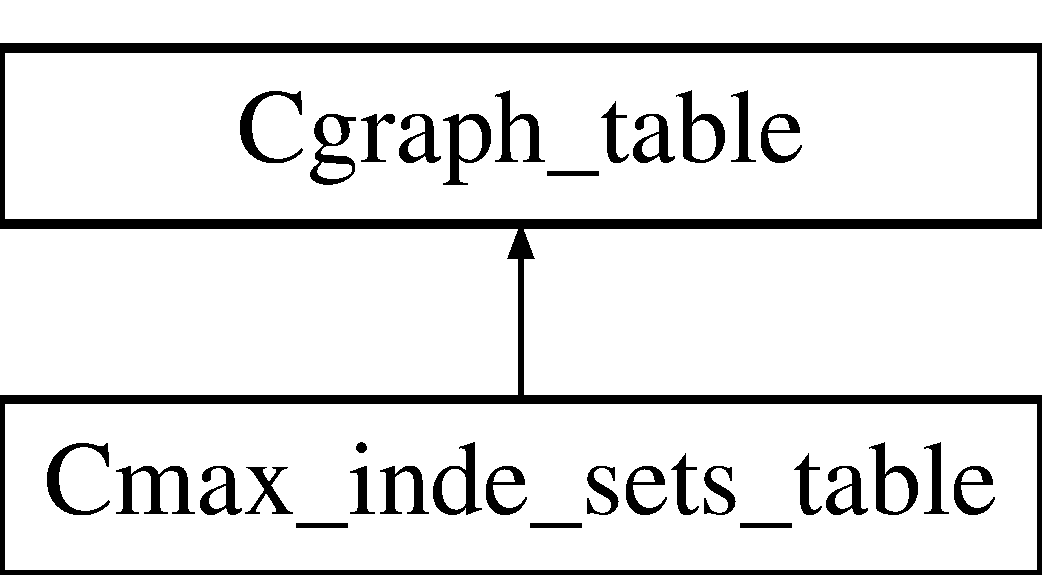
\includegraphics[height=2.000000cm]{class_cmax__inde__sets__table}
\end{center}
\end{figure}
\subsection*{Public Member Functions}
\begin{DoxyCompactItemize}
\item 
\hyperlink{class_cmax__inde__sets__table_a39fc5527f19ec28901ebc62407895dc9}{Cmax\+\_\+inde\+\_\+sets\+\_\+table} ()
\begin{DoxyCompactList}\small\item\em Purpose\+: create a new \hyperlink{class_cmax__inde__sets__table}{Cmax\+\_\+inde\+\_\+sets\+\_\+table} with null value. \end{DoxyCompactList}\item 
\hyperlink{class_cmax__inde__sets__table_ab80f89eb0991ad10c416082717822d9d}{$\sim$\+Cmax\+\_\+inde\+\_\+sets\+\_\+table} ()
\begin{DoxyCompactList}\small\item\em Purpose\+: delete a \hyperlink{class_cmax__inde__sets__table}{Cmax\+\_\+inde\+\_\+sets\+\_\+table} object , it remove all independant set in the list a free the object. \end{DoxyCompactList}\item 
unsigned int \hyperlink{class_cmax__inde__sets__table_a36ec7fecff6ba7547a936dbb964b9572}{M\+I\+Tget\+\_\+size\+\_\+max} ()
\begin{DoxyCompactList}\small\item\em Purpose\+: get the maximum size of the independant set of the list. \end{DoxyCompactList}\item 
void \hyperlink{class_cmax__inde__sets__table_ae5b5c5509b580597701d26d8a5a45faa}{G\+R\+Tempty\+\_\+table} ()
\begin{DoxyCompactList}\small\item\em Purpose\+: delete all the independant sets inside the table, and set the ui\+M\+I\+Tsize\+\_\+max to 0. \end{DoxyCompactList}\item 
void \hyperlink{class_cmax__inde__sets__table_a15a4bbf3ad99d6411cc79a2b3ab924c6}{M\+I\+Tenum\+\_\+max\+\_\+inde\+\_\+set} (\hyperlink{class_cgraph}{Cgraph} $\ast$p\+Graph, \hyperlink{class_cgraph}{Cgraph} $\ast$p\+Independant\+\_\+sets)
\begin{DoxyCompactList}\small\item\em Purpose\+: search all the maximum independant sets of a graph. \end{DoxyCompactList}\item 
void \hyperlink{class_cmax__inde__sets__table_ac1ea1bfbfe3c4dfdef3e966529f88c1f}{M\+I\+Tenum\+\_\+max\+\_\+inde\+\_\+set2} (\hyperlink{class_cgraph}{Cgraph} $\ast$p\+Graph, \hyperlink{class_cgraph}{Cgraph} $\ast$p\+Independant\+\_\+sets)
\item 
void \hyperlink{class_cmax__inde__sets__table_a4443b25faed663d6f2011d41edc30594}{M\+I\+Tenum\+\_\+max\+\_\+inde\+\_\+set3} (\hyperlink{class_cgraph}{Cgraph} $\ast$p\+Graph, \hyperlink{class_cgraph}{Cgraph} $\ast$p\+Independant\+\_\+sets)
\item 
void \hyperlink{class_cmax__inde__sets__table_ac97e4ba5939dd8a72c737ea4416997e2}{M\+I\+Tenum\+\_\+max\+\_\+inde\+\_\+set4} (\hyperlink{class_cgraph}{Cgraph} $\ast$p\+Graph)
\item 
void \hyperlink{class_cmax__inde__sets__table_a9365aa1408c211a8514e6a08c356c875}{M\+I\+Tenum\+\_\+max\+\_\+inde\+\_\+set5} (\hyperlink{class_cgraph}{Cgraph} $\ast$p\+Graph, \hyperlink{class_cgraph}{Cgraph} $\ast$p\+Independant\+\_\+sets)
\item 
void \hyperlink{class_cmax__inde__sets__table_a4945d82e35a9349f3299cf052e8454b1}{M\+I\+Tenum\+\_\+max\+\_\+inde\+\_\+set6} (\hyperlink{class_cgraph}{Cgraph} $\ast$p\+Graph, unsigned int ui\+Index\+\_\+current\+\_\+vertex)
\item 
void \hyperlink{class_cmax__inde__sets__table_ad02bc25918d717f721f9529836fa3a0a}{M\+I\+Tenum\+\_\+max\+\_\+inde\+\_\+set8} (\hyperlink{class_cgraph}{Cgraph} $\ast$p\+Graph, \hyperlink{class_cgraph}{Cgraph} $\ast$p\+Independant\+\_\+sets)
\item 
void \hyperlink{class_cmax__inde__sets__table_a0b912e6d883733b155f9c7064d8944a6}{M\+I\+Tenum\+\_\+max\+\_\+inde\+\_\+set7} (\hyperlink{class_cgraph}{Cgraph} $\ast$p\+Graph)
\item 
bool \hyperlink{class_cmax__inde__sets__table_ad6debe47c6f898406574908a34be3cc0}{M\+I\+Ttest\+\_\+if\+\_\+solution\+\_\+exist} (\hyperlink{class_cgraph}{Cgraph} $\ast$p\+Graph\+\_\+to\+\_\+compare)
\end{DoxyCompactItemize}
\subsection*{Private Attributes}
\begin{DoxyCompactItemize}
\item 
unsigned int \hyperlink{class_cmax__inde__sets__table_a9a847269f6dfaca3ce1c292fc31171cf}{ui\+M\+I\+Tsize\+\_\+max}
\end{DoxyCompactItemize}


\subsection{Detailed Description}
\hyperlink{class_cmax__inde__sets__table}{Cmax\+\_\+inde\+\_\+sets\+\_\+table} Class. 

Definition at line 16 of file Cmax\+\_\+inde\+\_\+sets\+\_\+table.\+h.



\subsection{Constructor \& Destructor Documentation}
\hypertarget{class_cmax__inde__sets__table_a39fc5527f19ec28901ebc62407895dc9}{}\index{Cmax\+\_\+inde\+\_\+sets\+\_\+table@{Cmax\+\_\+inde\+\_\+sets\+\_\+table}!Cmax\+\_\+inde\+\_\+sets\+\_\+table@{Cmax\+\_\+inde\+\_\+sets\+\_\+table}}
\index{Cmax\+\_\+inde\+\_\+sets\+\_\+table@{Cmax\+\_\+inde\+\_\+sets\+\_\+table}!Cmax\+\_\+inde\+\_\+sets\+\_\+table@{Cmax\+\_\+inde\+\_\+sets\+\_\+table}}
\subsubsection[{Cmax\+\_\+inde\+\_\+sets\+\_\+table}]{\setlength{\rightskip}{0pt plus 5cm}Cmax\+\_\+inde\+\_\+sets\+\_\+table\+::\+Cmax\+\_\+inde\+\_\+sets\+\_\+table (
\begin{DoxyParamCaption}
{}
\end{DoxyParamCaption}
)}\label{class_cmax__inde__sets__table_a39fc5527f19ec28901ebc62407895dc9}


Purpose\+: create a new \hyperlink{class_cmax__inde__sets__table}{Cmax\+\_\+inde\+\_\+sets\+\_\+table} with null value. 

\hyperlink{class_cmax__inde__sets__table_a39fc5527f19ec28901ebc62407895dc9}{Cmax\+\_\+inde\+\_\+sets\+\_\+table()} -\/ create a new \hyperlink{class_cmax__inde__sets__table}{Cmax\+\_\+inde\+\_\+sets\+\_\+table} with null value


\begin{DoxyParams}{Parameters}
{\em none} & \\
\hline
\end{DoxyParams}
\begin{DoxyReturn}{Returns}
none 
\end{DoxyReturn}


Definition at line 22 of file Cmax\+\_\+inde\+\_\+sets\+\_\+table.\+cpp.

\hypertarget{class_cmax__inde__sets__table_ab80f89eb0991ad10c416082717822d9d}{}\index{Cmax\+\_\+inde\+\_\+sets\+\_\+table@{Cmax\+\_\+inde\+\_\+sets\+\_\+table}!````~Cmax\+\_\+inde\+\_\+sets\+\_\+table@{$\sim$\+Cmax\+\_\+inde\+\_\+sets\+\_\+table}}
\index{````~Cmax\+\_\+inde\+\_\+sets\+\_\+table@{$\sim$\+Cmax\+\_\+inde\+\_\+sets\+\_\+table}!Cmax\+\_\+inde\+\_\+sets\+\_\+table@{Cmax\+\_\+inde\+\_\+sets\+\_\+table}}
\subsubsection[{$\sim$\+Cmax\+\_\+inde\+\_\+sets\+\_\+table}]{\setlength{\rightskip}{0pt plus 5cm}Cmax\+\_\+inde\+\_\+sets\+\_\+table\+::$\sim$\+Cmax\+\_\+inde\+\_\+sets\+\_\+table (
\begin{DoxyParamCaption}
{}
\end{DoxyParamCaption}
)}\label{class_cmax__inde__sets__table_ab80f89eb0991ad10c416082717822d9d}


Purpose\+: delete a \hyperlink{class_cmax__inde__sets__table}{Cmax\+\_\+inde\+\_\+sets\+\_\+table} object , it remove all independant set in the list a free the object. 

\hyperlink{class_cmax__inde__sets__table_ab80f89eb0991ad10c416082717822d9d}{$\sim$\+Cmax\+\_\+inde\+\_\+sets\+\_\+table()} -\/ delete correctly a \hyperlink{class_cmax__inde__sets__table}{Cmax\+\_\+inde\+\_\+sets\+\_\+table} object


\begin{DoxyParams}{Parameters}
{\em none} & \\
\hline
\end{DoxyParams}
\begin{DoxyReturn}{Returns}
none 
\end{DoxyReturn}


Definition at line 39 of file Cmax\+\_\+inde\+\_\+sets\+\_\+table.\+cpp.



\subsection{Member Function Documentation}
\hypertarget{class_cmax__inde__sets__table_ae5b5c5509b580597701d26d8a5a45faa}{}\index{Cmax\+\_\+inde\+\_\+sets\+\_\+table@{Cmax\+\_\+inde\+\_\+sets\+\_\+table}!G\+R\+Tempty\+\_\+table@{G\+R\+Tempty\+\_\+table}}
\index{G\+R\+Tempty\+\_\+table@{G\+R\+Tempty\+\_\+table}!Cmax\+\_\+inde\+\_\+sets\+\_\+table@{Cmax\+\_\+inde\+\_\+sets\+\_\+table}}
\subsubsection[{G\+R\+Tempty\+\_\+table}]{\setlength{\rightskip}{0pt plus 5cm}void Cmax\+\_\+inde\+\_\+sets\+\_\+table\+::\+G\+R\+Tempty\+\_\+table (
\begin{DoxyParamCaption}
{}
\end{DoxyParamCaption}
)}\label{class_cmax__inde__sets__table_ae5b5c5509b580597701d26d8a5a45faa}


Purpose\+: delete all the independant sets inside the table, and set the ui\+M\+I\+Tsize\+\_\+max to 0. 

void \hyperlink{class_cmax__inde__sets__table_ae5b5c5509b580597701d26d8a5a45faa}{G\+R\+Tempty\+\_\+table()} -\/ empty the table of independant sets


\begin{DoxyParams}{Parameters}
{\em none} & \\
\hline
\end{DoxyParams}
\begin{DoxyReturn}{Returns}
none 
\end{DoxyReturn}


Definition at line 73 of file Cmax\+\_\+inde\+\_\+sets\+\_\+table.\+cpp.

\hypertarget{class_cmax__inde__sets__table_a15a4bbf3ad99d6411cc79a2b3ab924c6}{}\index{Cmax\+\_\+inde\+\_\+sets\+\_\+table@{Cmax\+\_\+inde\+\_\+sets\+\_\+table}!M\+I\+Tenum\+\_\+max\+\_\+inde\+\_\+set@{M\+I\+Tenum\+\_\+max\+\_\+inde\+\_\+set}}
\index{M\+I\+Tenum\+\_\+max\+\_\+inde\+\_\+set@{M\+I\+Tenum\+\_\+max\+\_\+inde\+\_\+set}!Cmax\+\_\+inde\+\_\+sets\+\_\+table@{Cmax\+\_\+inde\+\_\+sets\+\_\+table}}
\subsubsection[{M\+I\+Tenum\+\_\+max\+\_\+inde\+\_\+set}]{\setlength{\rightskip}{0pt plus 5cm}void Cmax\+\_\+inde\+\_\+sets\+\_\+table\+::\+M\+I\+Tenum\+\_\+max\+\_\+inde\+\_\+set (
\begin{DoxyParamCaption}
\item[{{\bf Cgraph} $\ast$}]{p\+Graph, }
\item[{{\bf Cgraph} $\ast$}]{p\+Independant\+\_\+sets}
\end{DoxyParamCaption}
)}\label{class_cmax__inde__sets__table_a15a4bbf3ad99d6411cc79a2b3ab924c6}


Purpose\+: search all the maximum independant sets of a graph. 

void \hyperlink{class_cmax__inde__sets__table_a15a4bbf3ad99d6411cc79a2b3ab924c6}{M\+I\+Tenum\+\_\+max\+\_\+inde\+\_\+set(\+Cgraph $\ast$ p\+Graph, Cgraph $\ast$ p\+Independant\+\_\+sets)} -\/ search all the maximum independant sets of a graph


\begin{DoxyParams}{Parameters}
{\em \hyperlink{class_cgraph}{Cgraph}} & $\ast$ p\+Graph -\/ a graph , to determine independant sets \hyperlink{class_cgraph}{Cgraph} $\ast$ p\+Independant\+\_\+sets -\/ an independant set of the graph, N\+U\+L\+L if first call of the function.\\
\hline
\end{DoxyParams}
\begin{DoxyReturn}{Returns}
none 
\end{DoxyReturn}


Definition at line 92 of file Cmax\+\_\+inde\+\_\+sets\+\_\+table.\+cpp.

\hypertarget{class_cmax__inde__sets__table_ac1ea1bfbfe3c4dfdef3e966529f88c1f}{}\index{Cmax\+\_\+inde\+\_\+sets\+\_\+table@{Cmax\+\_\+inde\+\_\+sets\+\_\+table}!M\+I\+Tenum\+\_\+max\+\_\+inde\+\_\+set2@{M\+I\+Tenum\+\_\+max\+\_\+inde\+\_\+set2}}
\index{M\+I\+Tenum\+\_\+max\+\_\+inde\+\_\+set2@{M\+I\+Tenum\+\_\+max\+\_\+inde\+\_\+set2}!Cmax\+\_\+inde\+\_\+sets\+\_\+table@{Cmax\+\_\+inde\+\_\+sets\+\_\+table}}
\subsubsection[{M\+I\+Tenum\+\_\+max\+\_\+inde\+\_\+set2}]{\setlength{\rightskip}{0pt plus 5cm}void Cmax\+\_\+inde\+\_\+sets\+\_\+table\+::\+M\+I\+Tenum\+\_\+max\+\_\+inde\+\_\+set2 (
\begin{DoxyParamCaption}
\item[{{\bf Cgraph} $\ast$}]{p\+Graph, }
\item[{{\bf Cgraph} $\ast$}]{p\+Independant\+\_\+sets}
\end{DoxyParamCaption}
)}\label{class_cmax__inde__sets__table_ac1ea1bfbfe3c4dfdef3e966529f88c1f}


Definition at line 181 of file Cmax\+\_\+inde\+\_\+sets\+\_\+table.\+cpp.

\hypertarget{class_cmax__inde__sets__table_a4443b25faed663d6f2011d41edc30594}{}\index{Cmax\+\_\+inde\+\_\+sets\+\_\+table@{Cmax\+\_\+inde\+\_\+sets\+\_\+table}!M\+I\+Tenum\+\_\+max\+\_\+inde\+\_\+set3@{M\+I\+Tenum\+\_\+max\+\_\+inde\+\_\+set3}}
\index{M\+I\+Tenum\+\_\+max\+\_\+inde\+\_\+set3@{M\+I\+Tenum\+\_\+max\+\_\+inde\+\_\+set3}!Cmax\+\_\+inde\+\_\+sets\+\_\+table@{Cmax\+\_\+inde\+\_\+sets\+\_\+table}}
\subsubsection[{M\+I\+Tenum\+\_\+max\+\_\+inde\+\_\+set3}]{\setlength{\rightskip}{0pt plus 5cm}void Cmax\+\_\+inde\+\_\+sets\+\_\+table\+::\+M\+I\+Tenum\+\_\+max\+\_\+inde\+\_\+set3 (
\begin{DoxyParamCaption}
\item[{{\bf Cgraph} $\ast$}]{p\+Graph, }
\item[{{\bf Cgraph} $\ast$}]{p\+Independant\+\_\+sets}
\end{DoxyParamCaption}
)}\label{class_cmax__inde__sets__table_a4443b25faed663d6f2011d41edc30594}


Definition at line 226 of file Cmax\+\_\+inde\+\_\+sets\+\_\+table.\+cpp.

\hypertarget{class_cmax__inde__sets__table_ac97e4ba5939dd8a72c737ea4416997e2}{}\index{Cmax\+\_\+inde\+\_\+sets\+\_\+table@{Cmax\+\_\+inde\+\_\+sets\+\_\+table}!M\+I\+Tenum\+\_\+max\+\_\+inde\+\_\+set4@{M\+I\+Tenum\+\_\+max\+\_\+inde\+\_\+set4}}
\index{M\+I\+Tenum\+\_\+max\+\_\+inde\+\_\+set4@{M\+I\+Tenum\+\_\+max\+\_\+inde\+\_\+set4}!Cmax\+\_\+inde\+\_\+sets\+\_\+table@{Cmax\+\_\+inde\+\_\+sets\+\_\+table}}
\subsubsection[{M\+I\+Tenum\+\_\+max\+\_\+inde\+\_\+set4}]{\setlength{\rightskip}{0pt plus 5cm}void Cmax\+\_\+inde\+\_\+sets\+\_\+table\+::\+M\+I\+Tenum\+\_\+max\+\_\+inde\+\_\+set4 (
\begin{DoxyParamCaption}
\item[{{\bf Cgraph} $\ast$}]{p\+Graph}
\end{DoxyParamCaption}
)}\label{class_cmax__inde__sets__table_ac97e4ba5939dd8a72c737ea4416997e2}


Definition at line 327 of file Cmax\+\_\+inde\+\_\+sets\+\_\+table.\+cpp.

\hypertarget{class_cmax__inde__sets__table_a9365aa1408c211a8514e6a08c356c875}{}\index{Cmax\+\_\+inde\+\_\+sets\+\_\+table@{Cmax\+\_\+inde\+\_\+sets\+\_\+table}!M\+I\+Tenum\+\_\+max\+\_\+inde\+\_\+set5@{M\+I\+Tenum\+\_\+max\+\_\+inde\+\_\+set5}}
\index{M\+I\+Tenum\+\_\+max\+\_\+inde\+\_\+set5@{M\+I\+Tenum\+\_\+max\+\_\+inde\+\_\+set5}!Cmax\+\_\+inde\+\_\+sets\+\_\+table@{Cmax\+\_\+inde\+\_\+sets\+\_\+table}}
\subsubsection[{M\+I\+Tenum\+\_\+max\+\_\+inde\+\_\+set5}]{\setlength{\rightskip}{0pt plus 5cm}void Cmax\+\_\+inde\+\_\+sets\+\_\+table\+::\+M\+I\+Tenum\+\_\+max\+\_\+inde\+\_\+set5 (
\begin{DoxyParamCaption}
\item[{{\bf Cgraph} $\ast$}]{p\+Graph, }
\item[{{\bf Cgraph} $\ast$}]{p\+Independant\+\_\+sets}
\end{DoxyParamCaption}
)}\label{class_cmax__inde__sets__table_a9365aa1408c211a8514e6a08c356c875}


Definition at line 355 of file Cmax\+\_\+inde\+\_\+sets\+\_\+table.\+cpp.

\hypertarget{class_cmax__inde__sets__table_a4945d82e35a9349f3299cf052e8454b1}{}\index{Cmax\+\_\+inde\+\_\+sets\+\_\+table@{Cmax\+\_\+inde\+\_\+sets\+\_\+table}!M\+I\+Tenum\+\_\+max\+\_\+inde\+\_\+set6@{M\+I\+Tenum\+\_\+max\+\_\+inde\+\_\+set6}}
\index{M\+I\+Tenum\+\_\+max\+\_\+inde\+\_\+set6@{M\+I\+Tenum\+\_\+max\+\_\+inde\+\_\+set6}!Cmax\+\_\+inde\+\_\+sets\+\_\+table@{Cmax\+\_\+inde\+\_\+sets\+\_\+table}}
\subsubsection[{M\+I\+Tenum\+\_\+max\+\_\+inde\+\_\+set6}]{\setlength{\rightskip}{0pt plus 5cm}void Cmax\+\_\+inde\+\_\+sets\+\_\+table\+::\+M\+I\+Tenum\+\_\+max\+\_\+inde\+\_\+set6 (
\begin{DoxyParamCaption}
\item[{{\bf Cgraph} $\ast$}]{p\+Graph, }
\item[{unsigned int}]{ui\+Index\+\_\+current\+\_\+vertex}
\end{DoxyParamCaption}
)}\label{class_cmax__inde__sets__table_a4945d82e35a9349f3299cf052e8454b1}


Definition at line 405 of file Cmax\+\_\+inde\+\_\+sets\+\_\+table.\+cpp.

\hypertarget{class_cmax__inde__sets__table_a0b912e6d883733b155f9c7064d8944a6}{}\index{Cmax\+\_\+inde\+\_\+sets\+\_\+table@{Cmax\+\_\+inde\+\_\+sets\+\_\+table}!M\+I\+Tenum\+\_\+max\+\_\+inde\+\_\+set7@{M\+I\+Tenum\+\_\+max\+\_\+inde\+\_\+set7}}
\index{M\+I\+Tenum\+\_\+max\+\_\+inde\+\_\+set7@{M\+I\+Tenum\+\_\+max\+\_\+inde\+\_\+set7}!Cmax\+\_\+inde\+\_\+sets\+\_\+table@{Cmax\+\_\+inde\+\_\+sets\+\_\+table}}
\subsubsection[{M\+I\+Tenum\+\_\+max\+\_\+inde\+\_\+set7}]{\setlength{\rightskip}{0pt plus 5cm}void Cmax\+\_\+inde\+\_\+sets\+\_\+table\+::\+M\+I\+Tenum\+\_\+max\+\_\+inde\+\_\+set7 (
\begin{DoxyParamCaption}
\item[{{\bf Cgraph} $\ast$}]{p\+Graph}
\end{DoxyParamCaption}
)}\label{class_cmax__inde__sets__table_a0b912e6d883733b155f9c7064d8944a6}


Definition at line 450 of file Cmax\+\_\+inde\+\_\+sets\+\_\+table.\+cpp.

\hypertarget{class_cmax__inde__sets__table_ad02bc25918d717f721f9529836fa3a0a}{}\index{Cmax\+\_\+inde\+\_\+sets\+\_\+table@{Cmax\+\_\+inde\+\_\+sets\+\_\+table}!M\+I\+Tenum\+\_\+max\+\_\+inde\+\_\+set8@{M\+I\+Tenum\+\_\+max\+\_\+inde\+\_\+set8}}
\index{M\+I\+Tenum\+\_\+max\+\_\+inde\+\_\+set8@{M\+I\+Tenum\+\_\+max\+\_\+inde\+\_\+set8}!Cmax\+\_\+inde\+\_\+sets\+\_\+table@{Cmax\+\_\+inde\+\_\+sets\+\_\+table}}
\subsubsection[{M\+I\+Tenum\+\_\+max\+\_\+inde\+\_\+set8}]{\setlength{\rightskip}{0pt plus 5cm}void Cmax\+\_\+inde\+\_\+sets\+\_\+table\+::\+M\+I\+Tenum\+\_\+max\+\_\+inde\+\_\+set8 (
\begin{DoxyParamCaption}
\item[{{\bf Cgraph} $\ast$}]{p\+Graph, }
\item[{{\bf Cgraph} $\ast$}]{p\+Independant\+\_\+sets}
\end{DoxyParamCaption}
)}\label{class_cmax__inde__sets__table_ad02bc25918d717f721f9529836fa3a0a}


Definition at line 508 of file Cmax\+\_\+inde\+\_\+sets\+\_\+table.\+cpp.

\hypertarget{class_cmax__inde__sets__table_a36ec7fecff6ba7547a936dbb964b9572}{}\index{Cmax\+\_\+inde\+\_\+sets\+\_\+table@{Cmax\+\_\+inde\+\_\+sets\+\_\+table}!M\+I\+Tget\+\_\+size\+\_\+max@{M\+I\+Tget\+\_\+size\+\_\+max}}
\index{M\+I\+Tget\+\_\+size\+\_\+max@{M\+I\+Tget\+\_\+size\+\_\+max}!Cmax\+\_\+inde\+\_\+sets\+\_\+table@{Cmax\+\_\+inde\+\_\+sets\+\_\+table}}
\subsubsection[{M\+I\+Tget\+\_\+size\+\_\+max}]{\setlength{\rightskip}{0pt plus 5cm}unsigned int Cmax\+\_\+inde\+\_\+sets\+\_\+table\+::\+M\+I\+Tget\+\_\+size\+\_\+max (
\begin{DoxyParamCaption}
{}
\end{DoxyParamCaption}
)}\label{class_cmax__inde__sets__table_a36ec7fecff6ba7547a936dbb964b9572}


Purpose\+: get the maximum size of the independant set of the list. 

unsigned int \hyperlink{class_cmax__inde__sets__table_a36ec7fecff6ba7547a936dbb964b9572}{M\+I\+Tget\+\_\+size\+\_\+max()} -\/ get the maximum size of the independant set


\begin{DoxyParams}{Parameters}
{\em none} & \\
\hline
\end{DoxyParams}
\begin{DoxyReturn}{Returns}
unsigned int -\/ the maximum size of the independant set 
\end{DoxyReturn}


Definition at line 56 of file Cmax\+\_\+inde\+\_\+sets\+\_\+table.\+cpp.

\hypertarget{class_cmax__inde__sets__table_ad6debe47c6f898406574908a34be3cc0}{}\index{Cmax\+\_\+inde\+\_\+sets\+\_\+table@{Cmax\+\_\+inde\+\_\+sets\+\_\+table}!M\+I\+Ttest\+\_\+if\+\_\+solution\+\_\+exist@{M\+I\+Ttest\+\_\+if\+\_\+solution\+\_\+exist}}
\index{M\+I\+Ttest\+\_\+if\+\_\+solution\+\_\+exist@{M\+I\+Ttest\+\_\+if\+\_\+solution\+\_\+exist}!Cmax\+\_\+inde\+\_\+sets\+\_\+table@{Cmax\+\_\+inde\+\_\+sets\+\_\+table}}
\subsubsection[{M\+I\+Ttest\+\_\+if\+\_\+solution\+\_\+exist}]{\setlength{\rightskip}{0pt plus 5cm}bool Cmax\+\_\+inde\+\_\+sets\+\_\+table\+::\+M\+I\+Ttest\+\_\+if\+\_\+solution\+\_\+exist (
\begin{DoxyParamCaption}
\item[{{\bf Cgraph} $\ast$}]{p\+Graph\+\_\+to\+\_\+compare}
\end{DoxyParamCaption}
)}\label{class_cmax__inde__sets__table_ad6debe47c6f898406574908a34be3cc0}


Definition at line 601 of file Cmax\+\_\+inde\+\_\+sets\+\_\+table.\+cpp.



\subsection{Member Data Documentation}
\hypertarget{class_cmax__inde__sets__table_a9a847269f6dfaca3ce1c292fc31171cf}{}\index{Cmax\+\_\+inde\+\_\+sets\+\_\+table@{Cmax\+\_\+inde\+\_\+sets\+\_\+table}!ui\+M\+I\+Tsize\+\_\+max@{ui\+M\+I\+Tsize\+\_\+max}}
\index{ui\+M\+I\+Tsize\+\_\+max@{ui\+M\+I\+Tsize\+\_\+max}!Cmax\+\_\+inde\+\_\+sets\+\_\+table@{Cmax\+\_\+inde\+\_\+sets\+\_\+table}}
\subsubsection[{ui\+M\+I\+Tsize\+\_\+max}]{\setlength{\rightskip}{0pt plus 5cm}unsigned int Cmax\+\_\+inde\+\_\+sets\+\_\+table\+::ui\+M\+I\+Tsize\+\_\+max\hspace{0.3cm}{\ttfamily [private]}}\label{class_cmax__inde__sets__table_a9a847269f6dfaca3ce1c292fc31171cf}


Definition at line 18 of file Cmax\+\_\+inde\+\_\+sets\+\_\+table.\+h.



The documentation for this class was generated from the following files\+:\begin{DoxyCompactItemize}
\item 
Projet\+Cpp-\/\+Stable/\hyperlink{_cmax__inde__sets__table_8h}{Cmax\+\_\+inde\+\_\+sets\+\_\+table.\+h}\item 
Projet\+Cpp-\/\+Stable/\hyperlink{_cmax__inde__sets__table_8cpp}{Cmax\+\_\+inde\+\_\+sets\+\_\+table.\+cpp}\end{DoxyCompactItemize}

\hypertarget{class_cmax__inde__sets__table___u_n_i_t}{}\section{Cmax\+\_\+inde\+\_\+sets\+\_\+table\+\_\+\+U\+N\+I\+T Class Reference}
\label{class_cmax__inde__sets__table___u_n_i_t}\index{Cmax\+\_\+inde\+\_\+sets\+\_\+table\+\_\+\+U\+N\+I\+T@{Cmax\+\_\+inde\+\_\+sets\+\_\+table\+\_\+\+U\+N\+I\+T}}


\hyperlink{class_cmax__inde__sets__table___u_n_i_t}{Cmax\+\_\+inde\+\_\+sets\+\_\+table\+\_\+\+U\+N\+I\+T} Class.  




{\ttfamily \#include $<$Cmax\+\_\+inde\+\_\+sets\+\_\+table\+\_\+\+U\+N\+I\+T.\+h$>$}

\subsection*{Static Public Member Functions}
\begin{DoxyCompactItemize}
\item 
static void \hyperlink{class_cmax__inde__sets__table___u_n_i_t_a75bcff54dd34336b348593725f896877}{T\+E\+S\+T\+\_\+\+U\+N\+I\+T\+\_\+\+Cmax\+\_\+inde\+\_\+sets\+\_\+table\+\_\+\+U\+N\+I\+T} ()
\item 
static void \hyperlink{class_cmax__inde__sets__table___u_n_i_t_a18652790c12614ac78d0a284ce8b5e3d}{T\+E\+S\+T\+\_\+\+U\+N\+I\+T\+\_\+\+G\+R\+Tempty\+\_\+table} ()
\item 
static void \hyperlink{class_cmax__inde__sets__table___u_n_i_t_a798094cd2bdc9687bc180bbf6faa7678}{T\+E\+S\+T\+\_\+\+U\+N\+I\+T\+\_\+\+M\+I\+Tenum\+\_\+max\+\_\+inde\+\_\+set} ()
\end{DoxyCompactItemize}


\subsection{Detailed Description}
\hyperlink{class_cmax__inde__sets__table___u_n_i_t}{Cmax\+\_\+inde\+\_\+sets\+\_\+table\+\_\+\+U\+N\+I\+T} Class. 

Definition at line 13 of file Cmax\+\_\+inde\+\_\+sets\+\_\+table\+\_\+\+U\+N\+I\+T.\+h.



\subsection{Member Function Documentation}
\hypertarget{class_cmax__inde__sets__table___u_n_i_t_a75bcff54dd34336b348593725f896877}{}\index{Cmax\+\_\+inde\+\_\+sets\+\_\+table\+\_\+\+U\+N\+I\+T@{Cmax\+\_\+inde\+\_\+sets\+\_\+table\+\_\+\+U\+N\+I\+T}!T\+E\+S\+T\+\_\+\+U\+N\+I\+T\+\_\+\+Cmax\+\_\+inde\+\_\+sets\+\_\+table\+\_\+\+U\+N\+I\+T@{T\+E\+S\+T\+\_\+\+U\+N\+I\+T\+\_\+\+Cmax\+\_\+inde\+\_\+sets\+\_\+table\+\_\+\+U\+N\+I\+T}}
\index{T\+E\+S\+T\+\_\+\+U\+N\+I\+T\+\_\+\+Cmax\+\_\+inde\+\_\+sets\+\_\+table\+\_\+\+U\+N\+I\+T@{T\+E\+S\+T\+\_\+\+U\+N\+I\+T\+\_\+\+Cmax\+\_\+inde\+\_\+sets\+\_\+table\+\_\+\+U\+N\+I\+T}!Cmax\+\_\+inde\+\_\+sets\+\_\+table\+\_\+\+U\+N\+I\+T@{Cmax\+\_\+inde\+\_\+sets\+\_\+table\+\_\+\+U\+N\+I\+T}}
\subsubsection[{T\+E\+S\+T\+\_\+\+U\+N\+I\+T\+\_\+\+Cmax\+\_\+inde\+\_\+sets\+\_\+table\+\_\+\+U\+N\+I\+T}]{\setlength{\rightskip}{0pt plus 5cm}void Cmax\+\_\+inde\+\_\+sets\+\_\+table\+\_\+\+U\+N\+I\+T\+::\+T\+E\+S\+T\+\_\+\+U\+N\+I\+T\+\_\+\+Cmax\+\_\+inde\+\_\+sets\+\_\+table\+\_\+\+U\+N\+I\+T (
\begin{DoxyParamCaption}
{}
\end{DoxyParamCaption}
)\hspace{0.3cm}{\ttfamily [static]}}\label{class_cmax__inde__sets__table___u_n_i_t_a75bcff54dd34336b348593725f896877}


Definition at line 3 of file Cmax\+\_\+inde\+\_\+sets\+\_\+table\+\_\+\+U\+N\+I\+T.\+cpp.

\hypertarget{class_cmax__inde__sets__table___u_n_i_t_a18652790c12614ac78d0a284ce8b5e3d}{}\index{Cmax\+\_\+inde\+\_\+sets\+\_\+table\+\_\+\+U\+N\+I\+T@{Cmax\+\_\+inde\+\_\+sets\+\_\+table\+\_\+\+U\+N\+I\+T}!T\+E\+S\+T\+\_\+\+U\+N\+I\+T\+\_\+\+G\+R\+Tempty\+\_\+table@{T\+E\+S\+T\+\_\+\+U\+N\+I\+T\+\_\+\+G\+R\+Tempty\+\_\+table}}
\index{T\+E\+S\+T\+\_\+\+U\+N\+I\+T\+\_\+\+G\+R\+Tempty\+\_\+table@{T\+E\+S\+T\+\_\+\+U\+N\+I\+T\+\_\+\+G\+R\+Tempty\+\_\+table}!Cmax\+\_\+inde\+\_\+sets\+\_\+table\+\_\+\+U\+N\+I\+T@{Cmax\+\_\+inde\+\_\+sets\+\_\+table\+\_\+\+U\+N\+I\+T}}
\subsubsection[{T\+E\+S\+T\+\_\+\+U\+N\+I\+T\+\_\+\+G\+R\+Tempty\+\_\+table}]{\setlength{\rightskip}{0pt plus 5cm}void Cmax\+\_\+inde\+\_\+sets\+\_\+table\+\_\+\+U\+N\+I\+T\+::\+T\+E\+S\+T\+\_\+\+U\+N\+I\+T\+\_\+\+G\+R\+Tempty\+\_\+table (
\begin{DoxyParamCaption}
{}
\end{DoxyParamCaption}
)\hspace{0.3cm}{\ttfamily [static]}}\label{class_cmax__inde__sets__table___u_n_i_t_a18652790c12614ac78d0a284ce8b5e3d}


Definition at line 18 of file Cmax\+\_\+inde\+\_\+sets\+\_\+table\+\_\+\+U\+N\+I\+T.\+cpp.

\hypertarget{class_cmax__inde__sets__table___u_n_i_t_a798094cd2bdc9687bc180bbf6faa7678}{}\index{Cmax\+\_\+inde\+\_\+sets\+\_\+table\+\_\+\+U\+N\+I\+T@{Cmax\+\_\+inde\+\_\+sets\+\_\+table\+\_\+\+U\+N\+I\+T}!T\+E\+S\+T\+\_\+\+U\+N\+I\+T\+\_\+\+M\+I\+Tenum\+\_\+max\+\_\+inde\+\_\+set@{T\+E\+S\+T\+\_\+\+U\+N\+I\+T\+\_\+\+M\+I\+Tenum\+\_\+max\+\_\+inde\+\_\+set}}
\index{T\+E\+S\+T\+\_\+\+U\+N\+I\+T\+\_\+\+M\+I\+Tenum\+\_\+max\+\_\+inde\+\_\+set@{T\+E\+S\+T\+\_\+\+U\+N\+I\+T\+\_\+\+M\+I\+Tenum\+\_\+max\+\_\+inde\+\_\+set}!Cmax\+\_\+inde\+\_\+sets\+\_\+table\+\_\+\+U\+N\+I\+T@{Cmax\+\_\+inde\+\_\+sets\+\_\+table\+\_\+\+U\+N\+I\+T}}
\subsubsection[{T\+E\+S\+T\+\_\+\+U\+N\+I\+T\+\_\+\+M\+I\+Tenum\+\_\+max\+\_\+inde\+\_\+set}]{\setlength{\rightskip}{0pt plus 5cm}void Cmax\+\_\+inde\+\_\+sets\+\_\+table\+\_\+\+U\+N\+I\+T\+::\+T\+E\+S\+T\+\_\+\+U\+N\+I\+T\+\_\+\+M\+I\+Tenum\+\_\+max\+\_\+inde\+\_\+set (
\begin{DoxyParamCaption}
{}
\end{DoxyParamCaption}
)\hspace{0.3cm}{\ttfamily [static]}}\label{class_cmax__inde__sets__table___u_n_i_t_a798094cd2bdc9687bc180bbf6faa7678}


Definition at line 41 of file Cmax\+\_\+inde\+\_\+sets\+\_\+table\+\_\+\+U\+N\+I\+T.\+cpp.



The documentation for this class was generated from the following files\+:\begin{DoxyCompactItemize}
\item 
Projet\+Cpp-\/\+Stable/\hyperlink{_cmax__inde__sets__table___u_n_i_t_8h}{Cmax\+\_\+inde\+\_\+sets\+\_\+table\+\_\+\+U\+N\+I\+T.\+h}\item 
Projet\+Cpp-\/\+Stable/\hyperlink{_cmax__inde__sets__table___u_n_i_t_8cpp}{Cmax\+\_\+inde\+\_\+sets\+\_\+table\+\_\+\+U\+N\+I\+T.\+cpp}\end{DoxyCompactItemize}

\hypertarget{class_cvertex}{}\section{Cvertex Class Reference}
\label{class_cvertex}\index{Cvertex@{Cvertex}}


\hyperlink{class_cvertex}{Cvertex} Class.  




{\ttfamily \#include $<$Cvertex.\+h$>$}

\subsection*{Public Member Functions}
\begin{DoxyCompactItemize}
\item 
\hyperlink{class_cvertex_a4256affe77ee305afaf51aa9fcbd1cf0}{Cvertex} ()
\begin{DoxyCompactList}\small\item\em Purpose\+: allocate a new \hyperlink{class_cvertex}{Cvertex} and initialize it with null value. \end{DoxyCompactList}\item 
\hyperlink{class_cvertex_a3c091dc9431a4144f9d97767dd996186}{Cvertex} (const \hyperlink{class_cvertex}{Cvertex} \&vertex\+\_\+to\+\_\+copy)
\begin{DoxyCompactList}\small\item\em Purpose\+: create a new \hyperlink{class_cvertex}{Cvertex} with the value of another one. \end{DoxyCompactList}\item 
\hyperlink{class_cvertex_a9a4fa4f830633c4adabd066c75ca148d}{Cvertex} (unsigned int ui\+Id\+\_\+vertex, \hyperlink{class_cedges}{Cedges} $\ast$$\ast$pp\+List\+\_\+edges\+\_\+out, \hyperlink{class_cedges}{Cedges} $\ast$$\ast$pp\+List\+\_\+edges\+\_\+in, unsigned int ui\+Nb\+\_\+edges\+\_\+out, unsigned int ui\+Nb\+\_\+edges\+\_\+in)  throw (\+Cexception)
\begin{DoxyCompactList}\small\item\em Purpose\+: create a new \hyperlink{class_cvertex}{Cvertex} with the value in parameters pp\+List\+\_\+edges\+\_\+out, pp\+List\+\_\+edges\+\_\+in need to have a correct number of edge respectively in ui\+Nb\+\_\+edges\+\_\+out, ui\+Nb\+\_\+edges\+\_\+in. \end{DoxyCompactList}\item 
\hyperlink{class_cvertex_a91b564020e4c5b73f971f8d4e35dd952}{$\sim$\+Cvertex} ()
\begin{DoxyCompactList}\small\item\em Purpose\+: destroy a \hyperlink{class_cvertex}{Cvertex} correctly. \end{DoxyCompactList}\item 
void \hyperlink{class_cvertex_a6d76189e22c29a74cbae5a9a3507c312}{V\+E\+Rset\+\_\+id\+\_\+vertex} (unsigned int ui\+Id)
\begin{DoxyCompactList}\small\item\em Purpose\+: set the id of a vertex. \end{DoxyCompactList}\item 
void \hyperlink{class_cvertex_a0816cd7d37fe2ae4e6d347c98b5d603c}{V\+E\+Rset\+\_\+list\+\_\+edges\+\_\+out} (\hyperlink{class_cedges}{Cedges} $\ast$$\ast$pp\+List\+\_\+edges\+\_\+out, unsigned int ui\+Nb\+\_\+edges\+\_\+out)  throw (\+Cexception)
\begin{DoxyCompactList}\small\item\em Purpose\+: set the list of edge who go out the vertex pp\+List\+\_\+edges\+\_\+out need to have a correct number of edge ui\+Nb\+\_\+edges\+\_\+out. \end{DoxyCompactList}\item 
void \hyperlink{class_cvertex_a08f128a8c3988e24e62806f6655b4a37}{V\+E\+Rset\+\_\+list\+\_\+edges\+\_\+in} (\hyperlink{class_cedges}{Cedges} $\ast$$\ast$pp\+List\+\_\+edges\+\_\+in, unsigned int ui\+Nb\+\_\+edges\+\_\+in)  throw (\+Cexception)
\begin{DoxyCompactList}\small\item\em Purpose\+: set the list of edge who go in of the vertex pp\+List\+\_\+edges\+\_\+in need to have a correct number of edge ui\+Nb\+\_\+edges\+\_\+in. \end{DoxyCompactList}\item 
unsigned int \hyperlink{class_cvertex_ac2a86a2638f4b4ac43c9937aa76671a8}{V\+E\+Radd\+\_\+edge\+\_\+to\+\_\+list\+\_\+edges\+\_\+out} (\hyperlink{class_cedges}{Cedges} $\ast$p\+Edge\+\_\+to\+\_\+add)
\begin{DoxyCompactList}\small\item\em Purpose\+: add an edge to the list of edge who go out the vertex if the edge is already in the list it\textquotesingle{}s not added. \end{DoxyCompactList}\item 
unsigned int \hyperlink{class_cvertex_a49f2c7dde7f059ba1a03f60cac1dbecf}{V\+E\+Radd\+\_\+edge\+\_\+to\+\_\+list\+\_\+edges\+\_\+in} (\hyperlink{class_cedges}{Cedges} $\ast$p\+Edge\+\_\+to\+\_\+add)
\begin{DoxyCompactList}\small\item\em Purpose\+: add an edge to the list of edge who go in the vertex if the edge is already in the list it\textquotesingle{}s not added. \end{DoxyCompactList}\item 
\hyperlink{class_cedges}{Cedges} $\ast$ \hyperlink{class_cvertex_a44706c419e68981b586735e6af81edc1}{V\+E\+Rremove\+\_\+edge\+\_\+from\+\_\+list\+\_\+edges\+\_\+out} (unsigned int ui\+Id\+\_\+vertex\+\_\+out\+\_\+edge\+\_\+to\+\_\+delete)
\begin{DoxyCompactList}\small\item\em Purpose\+: remove an edge of the list of edge who go out the vertex if the edge is not in the list that return N\+U\+L\+L. \end{DoxyCompactList}\item 
\hyperlink{class_cedges}{Cedges} $\ast$ \hyperlink{class_cvertex_a4132709e06e653282a058fedb5274116}{V\+E\+Rremove\+\_\+edge\+\_\+from\+\_\+list\+\_\+edges\+\_\+in} (unsigned int ui\+Id\+\_\+vertex\+\_\+out\+\_\+edge\+\_\+to\+\_\+delete)
\begin{DoxyCompactList}\small\item\em Purpose\+: remove an edge of the list of edge who go in the vertex if the edge is not in the list that return N\+U\+L\+L. \end{DoxyCompactList}\item 
\hyperlink{class_cedges}{Cedges} $\ast$ \hyperlink{class_cvertex_ab699b9cc8727c4cef97ef26de16aaa0d}{V\+E\+Rremove\+\_\+edge\+\_\+from\+\_\+list\+\_\+edges\+\_\+out} (\hyperlink{class_cedges}{Cedges} $\ast$p\+Edge\+\_\+to\+\_\+delete)
\begin{DoxyCompactList}\small\item\em Purpose\+: remove an edge of the list of edge who go out the vertex if the edge is not in the list that return N\+U\+L\+L. \end{DoxyCompactList}\item 
\hyperlink{class_cedges}{Cedges} $\ast$ \hyperlink{class_cvertex_a49d5999465dd41b5d64f5339c2476272}{V\+E\+Rremove\+\_\+edge\+\_\+from\+\_\+list\+\_\+edges\+\_\+in} (\hyperlink{class_cedges}{Cedges} $\ast$p\+Edge\+\_\+to\+\_\+delete)
\begin{DoxyCompactList}\small\item\em Purpose\+: remove an edge of the list of edge who go in the vertex if the edge is not in the list that return N\+U\+L\+L. \end{DoxyCompactList}\item 
unsigned int \hyperlink{class_cvertex_a2091154529123d16fb0913c6a23f11c1}{V\+E\+Rfind\+\_\+index\+\_\+in\+\_\+list\+\_\+edge\+\_\+out} (\hyperlink{class_cedges}{Cedges} $\ast$p\+Edge\+\_\+to\+\_\+find)
\begin{DoxyCompactList}\small\item\em Purpose\+: find the index of a \hyperlink{class_cedges}{Cedges} in the list of edge who go out of the vertex. \end{DoxyCompactList}\item 
unsigned int \hyperlink{class_cvertex_a59f3b2cac925e322344e3158a762b8c5}{V\+E\+Rfind\+\_\+index\+\_\+in\+\_\+list\+\_\+edge\+\_\+in} (\hyperlink{class_cedges}{Cedges} $\ast$p\+Edge\+\_\+to\+\_\+find)
\begin{DoxyCompactList}\small\item\em Purpose\+: find the index of a \hyperlink{class_cedges}{Cedges} in the list of edge who go in of the vertex. \end{DoxyCompactList}\item 
unsigned int \hyperlink{class_cvertex_a65e2d9b32e91dbaf38fe44881b6eb425}{V\+E\+Rfind\+\_\+index\+\_\+in\+\_\+list\+\_\+edge\+\_\+out} (unsigned int ui\+Id\+\_\+vertex\+\_\+out\+\_\+edge\+\_\+to\+\_\+find)
\begin{DoxyCompactList}\small\item\em Purpose\+: find the index of a \hyperlink{class_cedges}{Cedges} in the list of edge who go out of the vertex. \end{DoxyCompactList}\item 
unsigned int \hyperlink{class_cvertex_ac3c85ea85f5abd32877f5bcae8fd012e}{V\+E\+Rfind\+\_\+index\+\_\+in\+\_\+list\+\_\+edge\+\_\+in} (unsigned int ui\+Id\+\_\+vertex\+\_\+out\+\_\+edge\+\_\+to\+\_\+find)
\begin{DoxyCompactList}\small\item\em Purpose\+: find the index of a \hyperlink{class_cedges}{Cedges} in the list of edge who go out of the vertex. \end{DoxyCompactList}\item 
unsigned int \hyperlink{class_cvertex_a3a792e08f085841355b57639e66bda1e}{V\+E\+Rget\+\_\+id\+\_\+vertex} ()
\begin{DoxyCompactList}\small\item\em Purpose\+: get the id of the vertex. \end{DoxyCompactList}\item 
\hyperlink{class_cedges}{Cedges} $\ast$$\ast$ \hyperlink{class_cvertex_a7e7923c919c93f15414b6c49b252a780}{V\+E\+Rget\+\_\+list\+\_\+edges\+\_\+out} ()
\begin{DoxyCompactList}\small\item\em Purpose\+: get the list of the edge who go out the vertex. \end{DoxyCompactList}\item 
\hyperlink{class_cedges}{Cedges} $\ast$$\ast$ \hyperlink{class_cvertex_a0bc728846b99cfd6f2cb5b9970927bfc}{V\+E\+Rget\+\_\+list\+\_\+edges\+\_\+in} ()
\begin{DoxyCompactList}\small\item\em Purpose\+: get the list of the edge who go in the vertex. \end{DoxyCompactList}\item 
unsigned int \hyperlink{class_cvertex_a887835cc19a342b774cf5426f27093c3}{V\+E\+Rget\+\_\+nb\+\_\+edges\+\_\+out} ()
\begin{DoxyCompactList}\small\item\em Purpose\+: get the number of edges who go out the vertex. \end{DoxyCompactList}\item 
unsigned int \hyperlink{class_cvertex_ab94674408a2d7c7bb651ab2ef0432d16}{V\+E\+Rget\+\_\+nb\+\_\+edges\+\_\+in} ()
\begin{DoxyCompactList}\small\item\em Purpose\+: get the number of edges who go in the vertex. \end{DoxyCompactList}\item 
unsigned int $\ast$ \hyperlink{class_cvertex_af741ade2dfb1c3b5839c2bdf1be1bff9}{V\+E\+Rget\+\_\+pred\+\_\+succ} ()
\item 
bool \hyperlink{class_cvertex_ad7afc0debf91cb6e6aae63a31439f5e9}{V\+E\+Ris\+\_\+vertex\+\_\+equivalent} (\hyperlink{class_cvertex}{Cvertex} $\ast$p\+Vertex\+To\+Compare)
\item 
\hyperlink{class_cvertex}{Cvertex} \& \hyperlink{class_cvertex_a8310facad7189774fd01cb2dcc4e975f}{operator=} (const \hyperlink{class_cvertex}{Cvertex} \&vertex\+To\+Copy)
\begin{DoxyCompactList}\small\item\em Purpose\+: enable the affectation of a \hyperlink{class_cvertex}{Cvertex} by another. \end{DoxyCompactList}\item 
bool \hyperlink{class_cvertex_a57b1f8e53f55ec33efdb7f62e9ea2584}{operator==} (\hyperlink{class_cvertex}{Cvertex} \&vertex\+To\+Compare)
\begin{DoxyCompactList}\small\item\em Purpose\+: compare two \hyperlink{class_cvertex}{Cvertex}. \end{DoxyCompactList}\item 
bool \hyperlink{class_cvertex_a2f3a0e226d96aacd1803e32278bd5930}{operator!=} (\hyperlink{class_cvertex}{Cvertex} \&vertex\+To\+Compare)
\begin{DoxyCompactList}\small\item\em Purpose\+: compare two \hyperlink{class_cvertex}{Cvertex}. \end{DoxyCompactList}\end{DoxyCompactItemize}
\subsection*{Private Attributes}
\begin{DoxyCompactItemize}
\item 
unsigned int \hyperlink{class_cvertex_ad10db8510c415314374789472f1436fc}{ui\+V\+E\+Rid\+\_\+vertex}
\item 
\hyperlink{class_cedges}{Cedges} $\ast$$\ast$ \hyperlink{class_cvertex_a4ab1d9ae28e17af0c8c3bc9da55d6e0a}{pp\+V\+E\+Rlist\+\_\+edges\+\_\+out}
\item 
\hyperlink{class_cedges}{Cedges} $\ast$$\ast$ \hyperlink{class_cvertex_a3a98de13fcfd72d549b013a4697b795e}{pp\+V\+E\+Rlist\+\_\+edges\+\_\+in}
\item 
unsigned int \hyperlink{class_cvertex_aefb09bb4a45f00a7de925bb63d2291a7}{ui\+V\+E\+Rnb\+\_\+edges\+\_\+in}
\item 
unsigned int \hyperlink{class_cvertex_a9b4b73496d3b28aef0912519d774572f}{ui\+V\+E\+Rnb\+\_\+edges\+\_\+out}
\end{DoxyCompactItemize}


\subsection{Detailed Description}
\hyperlink{class_cvertex}{Cvertex} Class. 

Definition at line 18 of file Cvertex.\+h.



\subsection{Constructor \& Destructor Documentation}
\hypertarget{class_cvertex_a4256affe77ee305afaf51aa9fcbd1cf0}{}\index{Cvertex@{Cvertex}!Cvertex@{Cvertex}}
\index{Cvertex@{Cvertex}!Cvertex@{Cvertex}}
\subsubsection[{Cvertex}]{\setlength{\rightskip}{0pt plus 5cm}Cvertex\+::\+Cvertex (
\begin{DoxyParamCaption}
{}
\end{DoxyParamCaption}
)}\label{class_cvertex_a4256affe77ee305afaf51aa9fcbd1cf0}


Purpose\+: allocate a new \hyperlink{class_cvertex}{Cvertex} and initialize it with null value. 

\hyperlink{class_cvertex_a4256affe77ee305afaf51aa9fcbd1cf0}{Cvertex()} -\/ allocate a new \hyperlink{class_cvertex}{Cvertex} and initialize it


\begin{DoxyParams}{Parameters}
{\em none} & \\
\hline
\end{DoxyParams}
\begin{DoxyReturn}{Returns}
none 
\end{DoxyReturn}


Definition at line 16 of file Cvertex.\+cpp.

\hypertarget{class_cvertex_a3c091dc9431a4144f9d97767dd996186}{}\index{Cvertex@{Cvertex}!Cvertex@{Cvertex}}
\index{Cvertex@{Cvertex}!Cvertex@{Cvertex}}
\subsubsection[{Cvertex}]{\setlength{\rightskip}{0pt plus 5cm}Cvertex\+::\+Cvertex (
\begin{DoxyParamCaption}
\item[{const {\bf Cvertex} \&}]{vertex\+\_\+to\+\_\+copy}
\end{DoxyParamCaption}
)}\label{class_cvertex_a3c091dc9431a4144f9d97767dd996186}


Purpose\+: create a new \hyperlink{class_cvertex}{Cvertex} with the value of another one. 

\hyperlink{class_cvertex_a4256affe77ee305afaf51aa9fcbd1cf0}{Cvertex()} -\/ create a new \hyperlink{class_cvertex}{Cvertex} with the value of another one


\begin{DoxyParams}{Parameters}
{\em const} & \hyperlink{class_cvertex}{Cvertex} \& vertex\+\_\+to\+\_\+copy -\/ the \hyperlink{class_cvertex}{Cvertex} to copy, if N\+U\+L\+L do the same as default constructor\\
\hline
\end{DoxyParams}
\begin{DoxyReturn}{Returns}
none 
\end{DoxyReturn}


Definition at line 33 of file Cvertex.\+cpp.

\hypertarget{class_cvertex_a9a4fa4f830633c4adabd066c75ca148d}{}\index{Cvertex@{Cvertex}!Cvertex@{Cvertex}}
\index{Cvertex@{Cvertex}!Cvertex@{Cvertex}}
\subsubsection[{Cvertex}]{\setlength{\rightskip}{0pt plus 5cm}Cvertex\+::\+Cvertex (
\begin{DoxyParamCaption}
\item[{unsigned int}]{ui\+Id\+\_\+vertex, }
\item[{{\bf Cedges} $\ast$$\ast$}]{pp\+List\+\_\+edges\+\_\+out, }
\item[{{\bf Cedges} $\ast$$\ast$}]{pp\+List\+\_\+edges\+\_\+in, }
\item[{unsigned int}]{ui\+Nb\+\_\+edges\+\_\+out, }
\item[{unsigned int}]{ui\+Nb\+\_\+edges\+\_\+in}
\end{DoxyParamCaption}
) throw  {\bf Cexception}) }\label{class_cvertex_a9a4fa4f830633c4adabd066c75ca148d}


Purpose\+: create a new \hyperlink{class_cvertex}{Cvertex} with the value in parameters pp\+List\+\_\+edges\+\_\+out, pp\+List\+\_\+edges\+\_\+in need to have a correct number of edge respectively in ui\+Nb\+\_\+edges\+\_\+out, ui\+Nb\+\_\+edges\+\_\+in. 

\hyperlink{class_cvertex_a4256affe77ee305afaf51aa9fcbd1cf0}{Cvertex()} -\/ create a new \hyperlink{class_cvertex}{Cvertex} with the value in parameters


\begin{DoxyParams}{Parameters}
{\em unsigned} & int ui\+Id\+\_\+vertex -\/ the id of the vertex \\
\hline
{\em \hyperlink{class_cedges}{Cedges}} & $\ast$$\ast$ pp\+List\+\_\+edges\+\_\+out -\/ the list of edges who go out the vertex \\
\hline
{\em \hyperlink{class_cedges}{Cedges}} & $\ast$$\ast$ pp\+List\+\_\+edges\+\_\+in -\/ the list of edges who go in the vertex \\
\hline
{\em unsigned} & int ui\+Nb\+\_\+edges\+\_\+out -\/ number of edges who go out the vertex \\
\hline
{\em unsigned} & int ui\+Nb\+\_\+edges\+\_\+in -\/ number of edges who go in the vertex\\
\hline
\end{DoxyParams}
\begin{DoxyReturn}{Returns}
none
\end{DoxyReturn}

\begin{DoxyExceptions}{Exceptions}
{\em E\+R\+R\+O\+R\+\_\+\+N\+U\+L\+L\+\_\+\+L\+I\+S\+T\+\_\+\+N\+B\+\_\+\+E\+L\+E\+M\+E\+N\+T\+\_\+\+N\+O\+T\+\_\+\+N\+U\+L\+L} & -\/ if one of the list in parameter is N\+U\+L\+L and the number of edges associated is not 0 \\
\hline
{\em E\+R\+R\+O\+R\+\_\+\+L\+I\+S\+T\+\_\+\+N\+O\+T\+\_\+\+N\+U\+L\+L} & -\/ if one of the list in parameter is not N\+U\+L\+L and the number of edges associated is 0 \\
\hline
\end{DoxyExceptions}


Definition at line 91 of file Cvertex.\+cpp.

\hypertarget{class_cvertex_a91b564020e4c5b73f971f8d4e35dd952}{}\index{Cvertex@{Cvertex}!````~Cvertex@{$\sim$\+Cvertex}}
\index{````~Cvertex@{$\sim$\+Cvertex}!Cvertex@{Cvertex}}
\subsubsection[{$\sim$\+Cvertex}]{\setlength{\rightskip}{0pt plus 5cm}Cvertex\+::$\sim$\+Cvertex (
\begin{DoxyParamCaption}
{}
\end{DoxyParamCaption}
)}\label{class_cvertex_a91b564020e4c5b73f971f8d4e35dd952}


Purpose\+: destroy a \hyperlink{class_cvertex}{Cvertex} correctly. 

\hyperlink{class_cvertex_a91b564020e4c5b73f971f8d4e35dd952}{$\sim$\+Cvertex()} -\/ destroy a \hyperlink{class_cvertex}{Cvertex} correctly


\begin{DoxyParams}{Parameters}
{\em none} & \\
\hline
\end{DoxyParams}
\begin{DoxyReturn}{Returns}
none 
\end{DoxyReturn}


Definition at line 140 of file Cvertex.\+cpp.



\subsection{Member Function Documentation}
\hypertarget{class_cvertex_a2f3a0e226d96aacd1803e32278bd5930}{}\index{Cvertex@{Cvertex}!operator"!=@{operator"!=}}
\index{operator"!=@{operator"!=}!Cvertex@{Cvertex}}
\subsubsection[{operator"!=}]{\setlength{\rightskip}{0pt plus 5cm}bool Cvertex\+::operator!= (
\begin{DoxyParamCaption}
\item[{{\bf Cvertex} \&}]{vertex\+To\+Compare}
\end{DoxyParamCaption}
)}\label{class_cvertex_a2f3a0e226d96aacd1803e32278bd5930}


Purpose\+: compare two \hyperlink{class_cvertex}{Cvertex}. 

operator!=(const Cvertex \&vertex\+\_\+to\+\_\+copy) -\/ compare two \hyperlink{class_cvertex}{Cvertex}


\begin{DoxyParams}{Parameters}
{\em \hyperlink{class_cvertex}{Cvertex}} & \& vertex\+To\+Compare -\/ the \hyperlink{class_cvertex}{Cvertex} to compare\\
\hline
\end{DoxyParams}
\begin{DoxyReturn}{Returns}
bool -\/ false if the two \hyperlink{class_cvertex}{Cvertex} are equal (in term of value not address), true if they are differents. 
\end{DoxyReturn}


Definition at line 862 of file Cvertex.\+cpp.

\hypertarget{class_cvertex_a8310facad7189774fd01cb2dcc4e975f}{}\index{Cvertex@{Cvertex}!operator=@{operator=}}
\index{operator=@{operator=}!Cvertex@{Cvertex}}
\subsubsection[{operator=}]{\setlength{\rightskip}{0pt plus 5cm}{\bf Cvertex} \& Cvertex\+::operator= (
\begin{DoxyParamCaption}
\item[{const {\bf Cvertex} \&}]{vertex\+To\+Copy}
\end{DoxyParamCaption}
)}\label{class_cvertex_a8310facad7189774fd01cb2dcc4e975f}


Purpose\+: enable the affectation of a \hyperlink{class_cvertex}{Cvertex} by another. 

\hyperlink{class_cvertex_a8310facad7189774fd01cb2dcc4e975f}{operator=(const Cvertex \&vertex\+\_\+to\+\_\+copy)} -\/ equal operator


\begin{DoxyParams}{Parameters}
{\em const} & \hyperlink{class_cvertex}{Cvertex} \& vertex\+\_\+to\+\_\+copy -\/ the \hyperlink{class_cvertex}{Cvertex} to copy\\
\hline
\end{DoxyParams}
\begin{DoxyReturn}{Returns}
\hyperlink{class_cvertex}{Cvertex} \& -\/ change the values of the object who call the operator 
\end{DoxyReturn}


Definition at line 773 of file Cvertex.\+cpp.

\hypertarget{class_cvertex_a57b1f8e53f55ec33efdb7f62e9ea2584}{}\index{Cvertex@{Cvertex}!operator==@{operator==}}
\index{operator==@{operator==}!Cvertex@{Cvertex}}
\subsubsection[{operator==}]{\setlength{\rightskip}{0pt plus 5cm}bool Cvertex\+::operator== (
\begin{DoxyParamCaption}
\item[{{\bf Cvertex} \&}]{vertex\+To\+Compare}
\end{DoxyParamCaption}
)}\label{class_cvertex_a57b1f8e53f55ec33efdb7f62e9ea2584}


Purpose\+: compare two \hyperlink{class_cvertex}{Cvertex}. 

operator==(const Cvertex \&vertex\+\_\+to\+\_\+copy) -\/ compare two \hyperlink{class_cvertex}{Cvertex}


\begin{DoxyParams}{Parameters}
{\em \hyperlink{class_cvertex}{Cvertex}} & \& vertex\+To\+Compare -\/ the \hyperlink{class_cvertex}{Cvertex} to compare\\
\hline
\end{DoxyParams}
\begin{DoxyReturn}{Returns}
bool -\/ true if the two \hyperlink{class_cvertex}{Cvertex} are equal (in term of value not address), false if they are differents. 
\end{DoxyReturn}


Definition at line 817 of file Cvertex.\+cpp.

\hypertarget{class_cvertex_a49f2c7dde7f059ba1a03f60cac1dbecf}{}\index{Cvertex@{Cvertex}!V\+E\+Radd\+\_\+edge\+\_\+to\+\_\+list\+\_\+edges\+\_\+in@{V\+E\+Radd\+\_\+edge\+\_\+to\+\_\+list\+\_\+edges\+\_\+in}}
\index{V\+E\+Radd\+\_\+edge\+\_\+to\+\_\+list\+\_\+edges\+\_\+in@{V\+E\+Radd\+\_\+edge\+\_\+to\+\_\+list\+\_\+edges\+\_\+in}!Cvertex@{Cvertex}}
\subsubsection[{V\+E\+Radd\+\_\+edge\+\_\+to\+\_\+list\+\_\+edges\+\_\+in}]{\setlength{\rightskip}{0pt plus 5cm}unsigned int Cvertex\+::\+V\+E\+Radd\+\_\+edge\+\_\+to\+\_\+list\+\_\+edges\+\_\+in (
\begin{DoxyParamCaption}
\item[{{\bf Cedges} $\ast$}]{p\+Edge\+\_\+to\+\_\+add}
\end{DoxyParamCaption}
)}\label{class_cvertex_a49f2c7dde7f059ba1a03f60cac1dbecf}


Purpose\+: add an edge to the list of edge who go in the vertex if the edge is already in the list it\textquotesingle{}s not added. 

\hyperlink{class_cvertex_a49f2c7dde7f059ba1a03f60cac1dbecf}{V\+E\+Radd\+\_\+edge\+\_\+to\+\_\+list\+\_\+edges\+\_\+in(\+Cedges $\ast$ p\+Edge\+\_\+to\+\_\+add)} -\/ add an edge to the list of edge who go in the vertex


\begin{DoxyParams}{Parameters}
{\em \hyperlink{class_cedges}{Cedges}} & $\ast$ p\+Edge\+\_\+to\+\_\+add -\/ the edge to add to the list\\
\hline
\end{DoxyParams}
\begin{DoxyReturn}{Returns}
unsigned int -\/ the position of the edge in the list 
\end{DoxyReturn}


Definition at line 352 of file Cvertex.\+cpp.

\hypertarget{class_cvertex_ac2a86a2638f4b4ac43c9937aa76671a8}{}\index{Cvertex@{Cvertex}!V\+E\+Radd\+\_\+edge\+\_\+to\+\_\+list\+\_\+edges\+\_\+out@{V\+E\+Radd\+\_\+edge\+\_\+to\+\_\+list\+\_\+edges\+\_\+out}}
\index{V\+E\+Radd\+\_\+edge\+\_\+to\+\_\+list\+\_\+edges\+\_\+out@{V\+E\+Radd\+\_\+edge\+\_\+to\+\_\+list\+\_\+edges\+\_\+out}!Cvertex@{Cvertex}}
\subsubsection[{V\+E\+Radd\+\_\+edge\+\_\+to\+\_\+list\+\_\+edges\+\_\+out}]{\setlength{\rightskip}{0pt plus 5cm}unsigned int Cvertex\+::\+V\+E\+Radd\+\_\+edge\+\_\+to\+\_\+list\+\_\+edges\+\_\+out (
\begin{DoxyParamCaption}
\item[{{\bf Cedges} $\ast$}]{p\+Edge\+\_\+to\+\_\+add}
\end{DoxyParamCaption}
)}\label{class_cvertex_ac2a86a2638f4b4ac43c9937aa76671a8}


Purpose\+: add an edge to the list of edge who go out the vertex if the edge is already in the list it\textquotesingle{}s not added. 

\hyperlink{class_cvertex_ac2a86a2638f4b4ac43c9937aa76671a8}{V\+E\+Radd\+\_\+edge\+\_\+to\+\_\+list\+\_\+edges\+\_\+out(\+Cedges $\ast$ p\+Edge\+\_\+to\+\_\+add)} -\/ add an edge to the list of edge who go out the vertex


\begin{DoxyParams}{Parameters}
{\em \hyperlink{class_cedges}{Cedges}} & $\ast$ p\+Edge\+\_\+to\+\_\+add -\/ the edge to add to the list\\
\hline
\end{DoxyParams}
\begin{DoxyReturn}{Returns}
unsigned int -\/ the position of the edge in the list 
\end{DoxyReturn}


Definition at line 312 of file Cvertex.\+cpp.

\hypertarget{class_cvertex_a59f3b2cac925e322344e3158a762b8c5}{}\index{Cvertex@{Cvertex}!V\+E\+Rfind\+\_\+index\+\_\+in\+\_\+list\+\_\+edge\+\_\+in@{V\+E\+Rfind\+\_\+index\+\_\+in\+\_\+list\+\_\+edge\+\_\+in}}
\index{V\+E\+Rfind\+\_\+index\+\_\+in\+\_\+list\+\_\+edge\+\_\+in@{V\+E\+Rfind\+\_\+index\+\_\+in\+\_\+list\+\_\+edge\+\_\+in}!Cvertex@{Cvertex}}
\subsubsection[{V\+E\+Rfind\+\_\+index\+\_\+in\+\_\+list\+\_\+edge\+\_\+in}]{\setlength{\rightskip}{0pt plus 5cm}unsigned int Cvertex\+::\+V\+E\+Rfind\+\_\+index\+\_\+in\+\_\+list\+\_\+edge\+\_\+in (
\begin{DoxyParamCaption}
\item[{{\bf Cedges} $\ast$}]{p\+Edge\+\_\+to\+\_\+find}
\end{DoxyParamCaption}
)}\label{class_cvertex_a59f3b2cac925e322344e3158a762b8c5}


Purpose\+: find the index of a \hyperlink{class_cedges}{Cedges} in the list of edge who go in of the vertex. 

\hyperlink{class_cvertex_a59f3b2cac925e322344e3158a762b8c5}{V\+E\+Rfind\+\_\+index\+\_\+in\+\_\+list\+\_\+edge\+\_\+in(\+Cedges $\ast$ p\+Edge\+\_\+to\+\_\+find)} -\/ find the index of a \hyperlink{class_cedges}{Cedges} in the list of edge who go in of the vertex


\begin{DoxyParams}{Parameters}
{\em \hyperlink{class_cedges}{Cedges}} & $\ast$ p\+Edge\+\_\+to\+\_\+find -\/ pointer on the edge to search\\
\hline
\end{DoxyParams}
\begin{DoxyReturn}{Returns}
unsigned in -\/ the index of the edge in the list, if the edge is not found return U\+I\+N\+T\+\_\+\+M\+A\+X 
\end{DoxyReturn}


Definition at line 561 of file Cvertex.\+cpp.

\hypertarget{class_cvertex_ac3c85ea85f5abd32877f5bcae8fd012e}{}\index{Cvertex@{Cvertex}!V\+E\+Rfind\+\_\+index\+\_\+in\+\_\+list\+\_\+edge\+\_\+in@{V\+E\+Rfind\+\_\+index\+\_\+in\+\_\+list\+\_\+edge\+\_\+in}}
\index{V\+E\+Rfind\+\_\+index\+\_\+in\+\_\+list\+\_\+edge\+\_\+in@{V\+E\+Rfind\+\_\+index\+\_\+in\+\_\+list\+\_\+edge\+\_\+in}!Cvertex@{Cvertex}}
\subsubsection[{V\+E\+Rfind\+\_\+index\+\_\+in\+\_\+list\+\_\+edge\+\_\+in}]{\setlength{\rightskip}{0pt plus 5cm}unsigned int Cvertex\+::\+V\+E\+Rfind\+\_\+index\+\_\+in\+\_\+list\+\_\+edge\+\_\+in (
\begin{DoxyParamCaption}
\item[{unsigned int}]{ui\+Id\+\_\+vertex\+\_\+out\+\_\+edge\+\_\+to\+\_\+find}
\end{DoxyParamCaption}
)}\label{class_cvertex_ac3c85ea85f5abd32877f5bcae8fd012e}


Purpose\+: find the index of a \hyperlink{class_cedges}{Cedges} in the list of edge who go out of the vertex. 

\hyperlink{class_cvertex_ac3c85ea85f5abd32877f5bcae8fd012e}{V\+E\+Rfind\+\_\+index\+\_\+in\+\_\+list\+\_\+edge\+\_\+in(unsigned int ui\+Id\+\_\+vertex\+\_\+out\+\_\+edge\+\_\+to\+\_\+find)} -\/ find the index of a \hyperlink{class_cedges}{Cedges} in the list of edge who go in of the vertex


\begin{DoxyParams}{Parameters}
{\em unsigned} & int ui\+Id\+\_\+vertex\+\_\+out\+\_\+edge\+\_\+to\+\_\+find -\/ id of the vertex inside the edge to search\\
\hline
\end{DoxyParams}
\begin{DoxyReturn}{Returns}
unsigned in -\/ the index of the edge in the list, if the edge is not found return U\+I\+N\+T\+\_\+\+M\+A\+X 
\end{DoxyReturn}


Definition at line 609 of file Cvertex.\+cpp.

\hypertarget{class_cvertex_a2091154529123d16fb0913c6a23f11c1}{}\index{Cvertex@{Cvertex}!V\+E\+Rfind\+\_\+index\+\_\+in\+\_\+list\+\_\+edge\+\_\+out@{V\+E\+Rfind\+\_\+index\+\_\+in\+\_\+list\+\_\+edge\+\_\+out}}
\index{V\+E\+Rfind\+\_\+index\+\_\+in\+\_\+list\+\_\+edge\+\_\+out@{V\+E\+Rfind\+\_\+index\+\_\+in\+\_\+list\+\_\+edge\+\_\+out}!Cvertex@{Cvertex}}
\subsubsection[{V\+E\+Rfind\+\_\+index\+\_\+in\+\_\+list\+\_\+edge\+\_\+out}]{\setlength{\rightskip}{0pt plus 5cm}unsigned int Cvertex\+::\+V\+E\+Rfind\+\_\+index\+\_\+in\+\_\+list\+\_\+edge\+\_\+out (
\begin{DoxyParamCaption}
\item[{{\bf Cedges} $\ast$}]{p\+Edge\+\_\+to\+\_\+find}
\end{DoxyParamCaption}
)}\label{class_cvertex_a2091154529123d16fb0913c6a23f11c1}


Purpose\+: find the index of a \hyperlink{class_cedges}{Cedges} in the list of edge who go out of the vertex. 

\hyperlink{class_cvertex_a2091154529123d16fb0913c6a23f11c1}{V\+E\+Rfind\+\_\+index\+\_\+in\+\_\+list\+\_\+edge\+\_\+out(\+Cedges $\ast$ p\+Edge\+\_\+to\+\_\+find)} -\/ find the index of a \hyperlink{class_cedges}{Cedges} in the list of edge who go out of the vertex


\begin{DoxyParams}{Parameters}
{\em \hyperlink{class_cedges}{Cedges}} & $\ast$ p\+Edge\+\_\+to\+\_\+find -\/ pointer on the edge to search\\
\hline
\end{DoxyParams}
\begin{DoxyReturn}{Returns}
unsigned in -\/ the index of the edge in the list, if the edge is not found return U\+I\+N\+T\+\_\+\+M\+A\+X 
\end{DoxyReturn}


Definition at line 536 of file Cvertex.\+cpp.

\hypertarget{class_cvertex_a65e2d9b32e91dbaf38fe44881b6eb425}{}\index{Cvertex@{Cvertex}!V\+E\+Rfind\+\_\+index\+\_\+in\+\_\+list\+\_\+edge\+\_\+out@{V\+E\+Rfind\+\_\+index\+\_\+in\+\_\+list\+\_\+edge\+\_\+out}}
\index{V\+E\+Rfind\+\_\+index\+\_\+in\+\_\+list\+\_\+edge\+\_\+out@{V\+E\+Rfind\+\_\+index\+\_\+in\+\_\+list\+\_\+edge\+\_\+out}!Cvertex@{Cvertex}}
\subsubsection[{V\+E\+Rfind\+\_\+index\+\_\+in\+\_\+list\+\_\+edge\+\_\+out}]{\setlength{\rightskip}{0pt plus 5cm}unsigned int Cvertex\+::\+V\+E\+Rfind\+\_\+index\+\_\+in\+\_\+list\+\_\+edge\+\_\+out (
\begin{DoxyParamCaption}
\item[{unsigned int}]{ui\+Id\+\_\+vertex\+\_\+out\+\_\+edge\+\_\+to\+\_\+find}
\end{DoxyParamCaption}
)}\label{class_cvertex_a65e2d9b32e91dbaf38fe44881b6eb425}


Purpose\+: find the index of a \hyperlink{class_cedges}{Cedges} in the list of edge who go out of the vertex. 

\hyperlink{class_cvertex_a65e2d9b32e91dbaf38fe44881b6eb425}{V\+E\+Rfind\+\_\+index\+\_\+in\+\_\+list\+\_\+edge\+\_\+out(unsigned int ui\+Id\+\_\+vertex\+\_\+out\+\_\+edge\+\_\+to\+\_\+find)} -\/ find the index of a \hyperlink{class_cedges}{Cedges} in the list of edge who go out of the vertex


\begin{DoxyParams}{Parameters}
{\em unsigned} & int ui\+Id\+\_\+vertex\+\_\+out\+\_\+edge\+\_\+to\+\_\+find -\/ id of the vertex inside the edge to search\\
\hline
\end{DoxyParams}
\begin{DoxyReturn}{Returns}
unsigned in -\/ the index of the edge in the list, if the edge is not found return U\+I\+N\+T\+\_\+\+M\+A\+X 
\end{DoxyReturn}


Definition at line 586 of file Cvertex.\+cpp.

\hypertarget{class_cvertex_a3a792e08f085841355b57639e66bda1e}{}\index{Cvertex@{Cvertex}!V\+E\+Rget\+\_\+id\+\_\+vertex@{V\+E\+Rget\+\_\+id\+\_\+vertex}}
\index{V\+E\+Rget\+\_\+id\+\_\+vertex@{V\+E\+Rget\+\_\+id\+\_\+vertex}!Cvertex@{Cvertex}}
\subsubsection[{V\+E\+Rget\+\_\+id\+\_\+vertex}]{\setlength{\rightskip}{0pt plus 5cm}unsigned int Cvertex\+::\+V\+E\+Rget\+\_\+id\+\_\+vertex (
\begin{DoxyParamCaption}
{}
\end{DoxyParamCaption}
)}\label{class_cvertex_a3a792e08f085841355b57639e66bda1e}


Purpose\+: get the id of the vertex. 

\hyperlink{class_cvertex_a3a792e08f085841355b57639e66bda1e}{V\+E\+Rget\+\_\+id\+\_\+vertex()} -\/ get the id of the vertex


\begin{DoxyParams}{Parameters}
{\em none} & \\
\hline
\end{DoxyParams}
\begin{DoxyReturn}{Returns}
unsigned in -\/ the id of the vertex 
\end{DoxyReturn}


Definition at line 629 of file Cvertex.\+cpp.

\hypertarget{class_cvertex_a0bc728846b99cfd6f2cb5b9970927bfc}{}\index{Cvertex@{Cvertex}!V\+E\+Rget\+\_\+list\+\_\+edges\+\_\+in@{V\+E\+Rget\+\_\+list\+\_\+edges\+\_\+in}}
\index{V\+E\+Rget\+\_\+list\+\_\+edges\+\_\+in@{V\+E\+Rget\+\_\+list\+\_\+edges\+\_\+in}!Cvertex@{Cvertex}}
\subsubsection[{V\+E\+Rget\+\_\+list\+\_\+edges\+\_\+in}]{\setlength{\rightskip}{0pt plus 5cm}{\bf Cedges} $\ast$$\ast$ Cvertex\+::\+V\+E\+Rget\+\_\+list\+\_\+edges\+\_\+in (
\begin{DoxyParamCaption}
{}
\end{DoxyParamCaption}
)}\label{class_cvertex_a0bc728846b99cfd6f2cb5b9970927bfc}


Purpose\+: get the list of the edge who go in the vertex. 

\hyperlink{class_cvertex_a7e7923c919c93f15414b6c49b252a780}{V\+E\+Rget\+\_\+list\+\_\+edges\+\_\+out()} -\/ get the list of the edge who go in the vertex

\begin{DoxyReturn}{Returns}
Cedges$\ast$$\ast$ -\/ the list of edges 
\end{DoxyReturn}


Definition at line 659 of file Cvertex.\+cpp.

\hypertarget{class_cvertex_a7e7923c919c93f15414b6c49b252a780}{}\index{Cvertex@{Cvertex}!V\+E\+Rget\+\_\+list\+\_\+edges\+\_\+out@{V\+E\+Rget\+\_\+list\+\_\+edges\+\_\+out}}
\index{V\+E\+Rget\+\_\+list\+\_\+edges\+\_\+out@{V\+E\+Rget\+\_\+list\+\_\+edges\+\_\+out}!Cvertex@{Cvertex}}
\subsubsection[{V\+E\+Rget\+\_\+list\+\_\+edges\+\_\+out}]{\setlength{\rightskip}{0pt plus 5cm}{\bf Cedges} $\ast$$\ast$ Cvertex\+::\+V\+E\+Rget\+\_\+list\+\_\+edges\+\_\+out (
\begin{DoxyParamCaption}
{}
\end{DoxyParamCaption}
)}\label{class_cvertex_a7e7923c919c93f15414b6c49b252a780}


Purpose\+: get the list of the edge who go out the vertex. 

\hyperlink{class_cvertex_a7e7923c919c93f15414b6c49b252a780}{V\+E\+Rget\+\_\+list\+\_\+edges\+\_\+out()} -\/ get the list of the edge who go out the vertex


\begin{DoxyParams}{Parameters}
{\em none} & \\
\hline
\end{DoxyParams}
\begin{DoxyReturn}{Returns}
Cedges$\ast$$\ast$ -\/ the list of edges 
\end{DoxyReturn}


Definition at line 644 of file Cvertex.\+cpp.

\hypertarget{class_cvertex_ab94674408a2d7c7bb651ab2ef0432d16}{}\index{Cvertex@{Cvertex}!V\+E\+Rget\+\_\+nb\+\_\+edges\+\_\+in@{V\+E\+Rget\+\_\+nb\+\_\+edges\+\_\+in}}
\index{V\+E\+Rget\+\_\+nb\+\_\+edges\+\_\+in@{V\+E\+Rget\+\_\+nb\+\_\+edges\+\_\+in}!Cvertex@{Cvertex}}
\subsubsection[{V\+E\+Rget\+\_\+nb\+\_\+edges\+\_\+in}]{\setlength{\rightskip}{0pt plus 5cm}unsigned int Cvertex\+::\+V\+E\+Rget\+\_\+nb\+\_\+edges\+\_\+in (
\begin{DoxyParamCaption}
{}
\end{DoxyParamCaption}
)}\label{class_cvertex_ab94674408a2d7c7bb651ab2ef0432d16}


Purpose\+: get the number of edges who go in the vertex. 

\hyperlink{class_cvertex_a887835cc19a342b774cf5426f27093c3}{V\+E\+Rget\+\_\+nb\+\_\+edges\+\_\+out()} -\/ get the number of edges who go in the vertex


\begin{DoxyParams}{Parameters}
{\em \hyperlink{class_cedges}{Cedges}} & $\ast$ p\+Edge\+\_\+to\+\_\+find -\/ the edge to search\\
\hline
\end{DoxyParams}
\begin{DoxyReturn}{Returns}
unsigned in -\/ the number of edges of the list 
\end{DoxyReturn}


Definition at line 695 of file Cvertex.\+cpp.

\hypertarget{class_cvertex_a887835cc19a342b774cf5426f27093c3}{}\index{Cvertex@{Cvertex}!V\+E\+Rget\+\_\+nb\+\_\+edges\+\_\+out@{V\+E\+Rget\+\_\+nb\+\_\+edges\+\_\+out}}
\index{V\+E\+Rget\+\_\+nb\+\_\+edges\+\_\+out@{V\+E\+Rget\+\_\+nb\+\_\+edges\+\_\+out}!Cvertex@{Cvertex}}
\subsubsection[{V\+E\+Rget\+\_\+nb\+\_\+edges\+\_\+out}]{\setlength{\rightskip}{0pt plus 5cm}unsigned int Cvertex\+::\+V\+E\+Rget\+\_\+nb\+\_\+edges\+\_\+out (
\begin{DoxyParamCaption}
{}
\end{DoxyParamCaption}
)}\label{class_cvertex_a887835cc19a342b774cf5426f27093c3}


Purpose\+: get the number of edges who go out the vertex. 

\hyperlink{class_cvertex_a887835cc19a342b774cf5426f27093c3}{V\+E\+Rget\+\_\+nb\+\_\+edges\+\_\+out()} -\/ get the number of edges who go out the vertex


\begin{DoxyParams}{Parameters}
{\em \hyperlink{class_cedges}{Cedges}} & $\ast$ p\+Edge\+\_\+to\+\_\+find -\/ the edge to search\\
\hline
\end{DoxyParams}
\begin{DoxyReturn}{Returns}
unsigned in -\/ the number of edges of the list 
\end{DoxyReturn}


Definition at line 677 of file Cvertex.\+cpp.

\hypertarget{class_cvertex_af741ade2dfb1c3b5839c2bdf1be1bff9}{}\index{Cvertex@{Cvertex}!V\+E\+Rget\+\_\+pred\+\_\+succ@{V\+E\+Rget\+\_\+pred\+\_\+succ}}
\index{V\+E\+Rget\+\_\+pred\+\_\+succ@{V\+E\+Rget\+\_\+pred\+\_\+succ}!Cvertex@{Cvertex}}
\subsubsection[{V\+E\+Rget\+\_\+pred\+\_\+succ}]{\setlength{\rightskip}{0pt plus 5cm}unsigned int $\ast$ Cvertex\+::\+V\+E\+Rget\+\_\+pred\+\_\+succ (
\begin{DoxyParamCaption}
{}
\end{DoxyParamCaption}
)}\label{class_cvertex_af741ade2dfb1c3b5839c2bdf1be1bff9}


Definition at line 699 of file Cvertex.\+cpp.

\hypertarget{class_cvertex_ad7afc0debf91cb6e6aae63a31439f5e9}{}\index{Cvertex@{Cvertex}!V\+E\+Ris\+\_\+vertex\+\_\+equivalent@{V\+E\+Ris\+\_\+vertex\+\_\+equivalent}}
\index{V\+E\+Ris\+\_\+vertex\+\_\+equivalent@{V\+E\+Ris\+\_\+vertex\+\_\+equivalent}!Cvertex@{Cvertex}}
\subsubsection[{V\+E\+Ris\+\_\+vertex\+\_\+equivalent}]{\setlength{\rightskip}{0pt plus 5cm}bool Cvertex\+::\+V\+E\+Ris\+\_\+vertex\+\_\+equivalent (
\begin{DoxyParamCaption}
\item[{{\bf Cvertex} $\ast$}]{p\+Vertex\+To\+Compare}
\end{DoxyParamCaption}
)}\label{class_cvertex_ad7afc0debf91cb6e6aae63a31439f5e9}


Definition at line 730 of file Cvertex.\+cpp.

\hypertarget{class_cvertex_a4132709e06e653282a058fedb5274116}{}\index{Cvertex@{Cvertex}!V\+E\+Rremove\+\_\+edge\+\_\+from\+\_\+list\+\_\+edges\+\_\+in@{V\+E\+Rremove\+\_\+edge\+\_\+from\+\_\+list\+\_\+edges\+\_\+in}}
\index{V\+E\+Rremove\+\_\+edge\+\_\+from\+\_\+list\+\_\+edges\+\_\+in@{V\+E\+Rremove\+\_\+edge\+\_\+from\+\_\+list\+\_\+edges\+\_\+in}!Cvertex@{Cvertex}}
\subsubsection[{V\+E\+Rremove\+\_\+edge\+\_\+from\+\_\+list\+\_\+edges\+\_\+in}]{\setlength{\rightskip}{0pt plus 5cm}{\bf Cedges} $\ast$ Cvertex\+::\+V\+E\+Rremove\+\_\+edge\+\_\+from\+\_\+list\+\_\+edges\+\_\+in (
\begin{DoxyParamCaption}
\item[{unsigned int}]{ui\+Id\+\_\+vertex\+\_\+out\+\_\+edge\+\_\+to\+\_\+delete}
\end{DoxyParamCaption}
)}\label{class_cvertex_a4132709e06e653282a058fedb5274116}


Purpose\+: remove an edge of the list of edge who go in the vertex if the edge is not in the list that return N\+U\+L\+L. 

\hyperlink{class_cvertex_a4132709e06e653282a058fedb5274116}{V\+E\+Rremove\+\_\+edge\+\_\+from\+\_\+list\+\_\+edges\+\_\+in(unsigned int ui\+Id\+\_\+vertex\+\_\+in\+\_\+edge\+\_\+to\+\_\+delete)} -\/ remove an edge of the list of edge who go in the vertex


\begin{DoxyParams}{Parameters}
{\em unsigned} & int ui\+Id\+\_\+vertex\+\_\+out\+\_\+edge\+\_\+to\+\_\+delete -\/ the Id of the vertex in the edge\\
\hline
\end{DoxyParams}
\begin{DoxyReturn}{Returns}
\hyperlink{class_cedges}{Cedges} $\ast$ -\/ if !\+N\+U\+L\+L a pointer on the \hyperlink{class_cedges}{Cedges} who has been successfully removed 
\end{DoxyReturn}


Definition at line 413 of file Cvertex.\+cpp.

\hypertarget{class_cvertex_a49d5999465dd41b5d64f5339c2476272}{}\index{Cvertex@{Cvertex}!V\+E\+Rremove\+\_\+edge\+\_\+from\+\_\+list\+\_\+edges\+\_\+in@{V\+E\+Rremove\+\_\+edge\+\_\+from\+\_\+list\+\_\+edges\+\_\+in}}
\index{V\+E\+Rremove\+\_\+edge\+\_\+from\+\_\+list\+\_\+edges\+\_\+in@{V\+E\+Rremove\+\_\+edge\+\_\+from\+\_\+list\+\_\+edges\+\_\+in}!Cvertex@{Cvertex}}
\subsubsection[{V\+E\+Rremove\+\_\+edge\+\_\+from\+\_\+list\+\_\+edges\+\_\+in}]{\setlength{\rightskip}{0pt plus 5cm}{\bf Cedges} $\ast$ Cvertex\+::\+V\+E\+Rremove\+\_\+edge\+\_\+from\+\_\+list\+\_\+edges\+\_\+in (
\begin{DoxyParamCaption}
\item[{{\bf Cedges} $\ast$}]{p\+Edge\+\_\+to\+\_\+delete}
\end{DoxyParamCaption}
)}\label{class_cvertex_a49d5999465dd41b5d64f5339c2476272}


Purpose\+: remove an edge of the list of edge who go in the vertex if the edge is not in the list that return N\+U\+L\+L. 

\hyperlink{class_cvertex_a4132709e06e653282a058fedb5274116}{V\+E\+Rremove\+\_\+edge\+\_\+from\+\_\+list\+\_\+edges\+\_\+in(unsigned int ui\+Id\+\_\+vertex\+\_\+in\+\_\+edge\+\_\+to\+\_\+delete)} -\/ remove an edge of the list of edge who go in the vertex


\begin{DoxyParams}{Parameters}
{\em \hyperlink{class_cedges}{Cedges}} & $\ast$ p\+Edge\+\_\+to\+\_\+delete -\/ pointer on the \hyperlink{class_cedges}{Cedges} to remove (this pointer don\textquotesingle{}t need to be a pointer on the \hyperlink{class_cedges}{Cedges} in the graph, but can be a copy of the \hyperlink{class_cedges}{Cedges})\\
\hline
\end{DoxyParams}
\begin{DoxyReturn}{Returns}
\hyperlink{class_cedges}{Cedges} $\ast$ -\/ if !\+N\+U\+L\+L a pointer on the \hyperlink{class_cedges}{Cedges} who has been successfully removed 
\end{DoxyReturn}


Definition at line 481 of file Cvertex.\+cpp.

\hypertarget{class_cvertex_a44706c419e68981b586735e6af81edc1}{}\index{Cvertex@{Cvertex}!V\+E\+Rremove\+\_\+edge\+\_\+from\+\_\+list\+\_\+edges\+\_\+out@{V\+E\+Rremove\+\_\+edge\+\_\+from\+\_\+list\+\_\+edges\+\_\+out}}
\index{V\+E\+Rremove\+\_\+edge\+\_\+from\+\_\+list\+\_\+edges\+\_\+out@{V\+E\+Rremove\+\_\+edge\+\_\+from\+\_\+list\+\_\+edges\+\_\+out}!Cvertex@{Cvertex}}
\subsubsection[{V\+E\+Rremove\+\_\+edge\+\_\+from\+\_\+list\+\_\+edges\+\_\+out}]{\setlength{\rightskip}{0pt plus 5cm}{\bf Cedges} $\ast$ Cvertex\+::\+V\+E\+Rremove\+\_\+edge\+\_\+from\+\_\+list\+\_\+edges\+\_\+out (
\begin{DoxyParamCaption}
\item[{unsigned int}]{ui\+Id\+\_\+vertex\+\_\+out\+\_\+edge\+\_\+to\+\_\+delete}
\end{DoxyParamCaption}
)}\label{class_cvertex_a44706c419e68981b586735e6af81edc1}


Purpose\+: remove an edge of the list of edge who go out the vertex if the edge is not in the list that return N\+U\+L\+L. 

\hyperlink{class_cvertex_a44706c419e68981b586735e6af81edc1}{V\+E\+Rremove\+\_\+edge\+\_\+from\+\_\+list\+\_\+edges\+\_\+out(unsigned int ui\+Id\+\_\+vertex\+\_\+out\+\_\+edge\+\_\+to\+\_\+delete)} -\/ remove an edge of the list of edge who go out the vertex


\begin{DoxyParams}{Parameters}
{\em unsigned} & int ui\+Id\+\_\+vertex\+\_\+out\+\_\+edge\+\_\+to\+\_\+delete -\/ the Id of the vertex in the edge\\
\hline
\end{DoxyParams}
\begin{DoxyReturn}{Returns}
\hyperlink{class_cedges}{Cedges} $\ast$ -\/ if !\+N\+U\+L\+L a pointer on the \hyperlink{class_cedges}{Cedges} who has been successfully removed 
\end{DoxyReturn}


Definition at line 391 of file Cvertex.\+cpp.

\hypertarget{class_cvertex_ab699b9cc8727c4cef97ef26de16aaa0d}{}\index{Cvertex@{Cvertex}!V\+E\+Rremove\+\_\+edge\+\_\+from\+\_\+list\+\_\+edges\+\_\+out@{V\+E\+Rremove\+\_\+edge\+\_\+from\+\_\+list\+\_\+edges\+\_\+out}}
\index{V\+E\+Rremove\+\_\+edge\+\_\+from\+\_\+list\+\_\+edges\+\_\+out@{V\+E\+Rremove\+\_\+edge\+\_\+from\+\_\+list\+\_\+edges\+\_\+out}!Cvertex@{Cvertex}}
\subsubsection[{V\+E\+Rremove\+\_\+edge\+\_\+from\+\_\+list\+\_\+edges\+\_\+out}]{\setlength{\rightskip}{0pt plus 5cm}{\bf Cedges} $\ast$ Cvertex\+::\+V\+E\+Rremove\+\_\+edge\+\_\+from\+\_\+list\+\_\+edges\+\_\+out (
\begin{DoxyParamCaption}
\item[{{\bf Cedges} $\ast$}]{p\+Edge\+\_\+to\+\_\+delete}
\end{DoxyParamCaption}
)}\label{class_cvertex_ab699b9cc8727c4cef97ef26de16aaa0d}


Purpose\+: remove an edge of the list of edge who go out the vertex if the edge is not in the list that return N\+U\+L\+L. 

\hyperlink{class_cvertex_a44706c419e68981b586735e6af81edc1}{V\+E\+Rremove\+\_\+edge\+\_\+from\+\_\+list\+\_\+edges\+\_\+out(unsigned int ui\+Id\+\_\+vertex\+\_\+out\+\_\+edge\+\_\+to\+\_\+delete)} -\/ remove an edge of the list of edge who go out the vertex


\begin{DoxyParams}{Parameters}
{\em \hyperlink{class_cedges}{Cedges}} & $\ast$ p\+Edge\+\_\+to\+\_\+delete -\/ pointer on the \hyperlink{class_cedges}{Cedges} to remove (this pointer don\textquotesingle{}t need to be a pointer on the \hyperlink{class_cedges}{Cedges} in the graph, but can be a copy of the \hyperlink{class_cedges}{Cedges})\\
\hline
\end{DoxyParams}
\begin{DoxyReturn}{Returns}
\hyperlink{class_cedges}{Cedges} $\ast$ -\/ if !\+N\+U\+L\+L a pointer on the \hyperlink{class_cedges}{Cedges} who has been successfully removed 
\end{DoxyReturn}


Definition at line 436 of file Cvertex.\+cpp.

\hypertarget{class_cvertex_a6d76189e22c29a74cbae5a9a3507c312}{}\index{Cvertex@{Cvertex}!V\+E\+Rset\+\_\+id\+\_\+vertex@{V\+E\+Rset\+\_\+id\+\_\+vertex}}
\index{V\+E\+Rset\+\_\+id\+\_\+vertex@{V\+E\+Rset\+\_\+id\+\_\+vertex}!Cvertex@{Cvertex}}
\subsubsection[{V\+E\+Rset\+\_\+id\+\_\+vertex}]{\setlength{\rightskip}{0pt plus 5cm}void Cvertex\+::\+V\+E\+Rset\+\_\+id\+\_\+vertex (
\begin{DoxyParamCaption}
\item[{unsigned int}]{ui\+Id}
\end{DoxyParamCaption}
)}\label{class_cvertex_a6d76189e22c29a74cbae5a9a3507c312}


Purpose\+: set the id of a vertex. 

\hyperlink{class_cvertex_a6d76189e22c29a74cbae5a9a3507c312}{V\+E\+Rset\+\_\+id\+\_\+vertex(unsigned int ui\+Id)} -\/ set the id of a vertex


\begin{DoxyParams}{Parameters}
{\em unsigned} & int ui\+Id -\/ the id of the vertex\\
\hline
\end{DoxyParams}
\begin{DoxyReturn}{Returns}
none 
\end{DoxyReturn}


Definition at line 185 of file Cvertex.\+cpp.

\hypertarget{class_cvertex_a08f128a8c3988e24e62806f6655b4a37}{}\index{Cvertex@{Cvertex}!V\+E\+Rset\+\_\+list\+\_\+edges\+\_\+in@{V\+E\+Rset\+\_\+list\+\_\+edges\+\_\+in}}
\index{V\+E\+Rset\+\_\+list\+\_\+edges\+\_\+in@{V\+E\+Rset\+\_\+list\+\_\+edges\+\_\+in}!Cvertex@{Cvertex}}
\subsubsection[{V\+E\+Rset\+\_\+list\+\_\+edges\+\_\+in}]{\setlength{\rightskip}{0pt plus 5cm}void Cvertex\+::\+V\+E\+Rset\+\_\+list\+\_\+edges\+\_\+in (
\begin{DoxyParamCaption}
\item[{{\bf Cedges} $\ast$$\ast$}]{pp\+List\+\_\+edges\+\_\+in, }
\item[{unsigned int}]{ui\+Nb\+\_\+edges\+\_\+in}
\end{DoxyParamCaption}
) throw  {\bf Cexception}) }\label{class_cvertex_a08f128a8c3988e24e62806f6655b4a37}


Purpose\+: set the list of edge who go in of the vertex pp\+List\+\_\+edges\+\_\+in need to have a correct number of edge ui\+Nb\+\_\+edges\+\_\+in. 

\hyperlink{class_cvertex_a08f128a8c3988e24e62806f6655b4a37}{V\+E\+Rset\+\_\+list\+\_\+edges\+\_\+in(\+Cedges$\ast$$\ast$ pp\+List\+\_\+edges\+\_\+in, unsigned int ui\+Nb\+\_\+edges\+\_\+in)} -\/ set the list of edge who go in the vertex


\begin{DoxyParams}{Parameters}
{\em \hyperlink{class_cedges}{Cedges}} & $\ast$$\ast$ pp\+List\+\_\+edges\+\_\+in -\/ the list of edges who go in the vertex \\
\hline
{\em unsigned} & int ui\+Nb\+\_\+edges\+\_\+in -\/ number of edges who go in the vertex\\
\hline
\end{DoxyParams}
\begin{DoxyReturn}{Returns}
none
\end{DoxyReturn}

\begin{DoxyExceptions}{Exceptions}
{\em E\+R\+R\+O\+R\+\_\+\+N\+U\+L\+L\+\_\+\+L\+I\+S\+T\+\_\+\+N\+B\+\_\+\+E\+L\+E\+M\+E\+N\+T\+\_\+\+N\+O\+T\+\_\+\+N\+U\+L\+L} & -\/ if the list in parameter is N\+U\+L\+L and the number of edges associated is not 0 E\+R\+R\+O\+R\+\_\+\+L\+I\+S\+T\+\_\+\+N\+O\+T\+\_\+\+N\+U\+L\+L -\/ if the list in parameter is not N\+U\+L\+L and the number of edges associated is 0 \\
\hline
\end{DoxyExceptions}


Definition at line 264 of file Cvertex.\+cpp.

\hypertarget{class_cvertex_a0816cd7d37fe2ae4e6d347c98b5d603c}{}\index{Cvertex@{Cvertex}!V\+E\+Rset\+\_\+list\+\_\+edges\+\_\+out@{V\+E\+Rset\+\_\+list\+\_\+edges\+\_\+out}}
\index{V\+E\+Rset\+\_\+list\+\_\+edges\+\_\+out@{V\+E\+Rset\+\_\+list\+\_\+edges\+\_\+out}!Cvertex@{Cvertex}}
\subsubsection[{V\+E\+Rset\+\_\+list\+\_\+edges\+\_\+out}]{\setlength{\rightskip}{0pt plus 5cm}void Cvertex\+::\+V\+E\+Rset\+\_\+list\+\_\+edges\+\_\+out (
\begin{DoxyParamCaption}
\item[{{\bf Cedges} $\ast$$\ast$}]{pp\+List\+\_\+edges\+\_\+out, }
\item[{unsigned int}]{ui\+Nb\+\_\+edges\+\_\+out}
\end{DoxyParamCaption}
) throw  {\bf Cexception}) }\label{class_cvertex_a0816cd7d37fe2ae4e6d347c98b5d603c}


Purpose\+: set the list of edge who go out the vertex pp\+List\+\_\+edges\+\_\+out need to have a correct number of edge ui\+Nb\+\_\+edges\+\_\+out. 

\hyperlink{class_cvertex_a0816cd7d37fe2ae4e6d347c98b5d603c}{V\+E\+Rset\+\_\+list\+\_\+edges\+\_\+out(\+Cedges$\ast$$\ast$ pp\+List\+\_\+edges\+\_\+out, unsigned int ui\+Nb\+\_\+edges\+\_\+out)} -\/ set the list of edge who go out the vertex


\begin{DoxyParams}{Parameters}
{\em \hyperlink{class_cedges}{Cedges}} & $\ast$$\ast$ pp\+List\+\_\+edges\+\_\+out -\/ the list of edges who go out the vertex \\
\hline
{\em unsigned} & int ui\+Nb\+\_\+edges\+\_\+out -\/ number of edges who go out the vertex\\
\hline
\end{DoxyParams}
\begin{DoxyReturn}{Returns}
none \begin{DoxyVerb}rows
    ERROR_NULL_LIST_NB_ELEMENT_NOT_NULL -   if the list in parameter is NULL and the number of edges associated is not 0
    ERROR_LIST_NOT_NULL                 -   if the list in parameter is not NULL and the number of edges associated is 0\end{DoxyVerb}
 
\end{DoxyReturn}


Definition at line 208 of file Cvertex.\+cpp.



\subsection{Member Data Documentation}
\hypertarget{class_cvertex_a3a98de13fcfd72d549b013a4697b795e}{}\index{Cvertex@{Cvertex}!pp\+V\+E\+Rlist\+\_\+edges\+\_\+in@{pp\+V\+E\+Rlist\+\_\+edges\+\_\+in}}
\index{pp\+V\+E\+Rlist\+\_\+edges\+\_\+in@{pp\+V\+E\+Rlist\+\_\+edges\+\_\+in}!Cvertex@{Cvertex}}
\subsubsection[{pp\+V\+E\+Rlist\+\_\+edges\+\_\+in}]{\setlength{\rightskip}{0pt plus 5cm}{\bf Cedges}$\ast$$\ast$ Cvertex\+::pp\+V\+E\+Rlist\+\_\+edges\+\_\+in\hspace{0.3cm}{\ttfamily [private]}}\label{class_cvertex_a3a98de13fcfd72d549b013a4697b795e}


Definition at line 25 of file Cvertex.\+h.

\hypertarget{class_cvertex_a4ab1d9ae28e17af0c8c3bc9da55d6e0a}{}\index{Cvertex@{Cvertex}!pp\+V\+E\+Rlist\+\_\+edges\+\_\+out@{pp\+V\+E\+Rlist\+\_\+edges\+\_\+out}}
\index{pp\+V\+E\+Rlist\+\_\+edges\+\_\+out@{pp\+V\+E\+Rlist\+\_\+edges\+\_\+out}!Cvertex@{Cvertex}}
\subsubsection[{pp\+V\+E\+Rlist\+\_\+edges\+\_\+out}]{\setlength{\rightskip}{0pt plus 5cm}{\bf Cedges}$\ast$$\ast$ Cvertex\+::pp\+V\+E\+Rlist\+\_\+edges\+\_\+out\hspace{0.3cm}{\ttfamily [private]}}\label{class_cvertex_a4ab1d9ae28e17af0c8c3bc9da55d6e0a}


Definition at line 23 of file Cvertex.\+h.

\hypertarget{class_cvertex_ad10db8510c415314374789472f1436fc}{}\index{Cvertex@{Cvertex}!ui\+V\+E\+Rid\+\_\+vertex@{ui\+V\+E\+Rid\+\_\+vertex}}
\index{ui\+V\+E\+Rid\+\_\+vertex@{ui\+V\+E\+Rid\+\_\+vertex}!Cvertex@{Cvertex}}
\subsubsection[{ui\+V\+E\+Rid\+\_\+vertex}]{\setlength{\rightskip}{0pt plus 5cm}unsigned int Cvertex\+::ui\+V\+E\+Rid\+\_\+vertex\hspace{0.3cm}{\ttfamily [private]}}\label{class_cvertex_ad10db8510c415314374789472f1436fc}


Definition at line 21 of file Cvertex.\+h.

\hypertarget{class_cvertex_aefb09bb4a45f00a7de925bb63d2291a7}{}\index{Cvertex@{Cvertex}!ui\+V\+E\+Rnb\+\_\+edges\+\_\+in@{ui\+V\+E\+Rnb\+\_\+edges\+\_\+in}}
\index{ui\+V\+E\+Rnb\+\_\+edges\+\_\+in@{ui\+V\+E\+Rnb\+\_\+edges\+\_\+in}!Cvertex@{Cvertex}}
\subsubsection[{ui\+V\+E\+Rnb\+\_\+edges\+\_\+in}]{\setlength{\rightskip}{0pt plus 5cm}unsigned int Cvertex\+::ui\+V\+E\+Rnb\+\_\+edges\+\_\+in\hspace{0.3cm}{\ttfamily [private]}}\label{class_cvertex_aefb09bb4a45f00a7de925bb63d2291a7}


Definition at line 27 of file Cvertex.\+h.

\hypertarget{class_cvertex_a9b4b73496d3b28aef0912519d774572f}{}\index{Cvertex@{Cvertex}!ui\+V\+E\+Rnb\+\_\+edges\+\_\+out@{ui\+V\+E\+Rnb\+\_\+edges\+\_\+out}}
\index{ui\+V\+E\+Rnb\+\_\+edges\+\_\+out@{ui\+V\+E\+Rnb\+\_\+edges\+\_\+out}!Cvertex@{Cvertex}}
\subsubsection[{ui\+V\+E\+Rnb\+\_\+edges\+\_\+out}]{\setlength{\rightskip}{0pt plus 5cm}unsigned int Cvertex\+::ui\+V\+E\+Rnb\+\_\+edges\+\_\+out\hspace{0.3cm}{\ttfamily [private]}}\label{class_cvertex_a9b4b73496d3b28aef0912519d774572f}


Definition at line 29 of file Cvertex.\+h.



The documentation for this class was generated from the following files\+:\begin{DoxyCompactItemize}
\item 
Projet\+Cpp-\/\+Stable/\hyperlink{_cvertex_8h}{Cvertex.\+h}\item 
Projet\+Cpp-\/\+Stable/\hyperlink{_cvertex_8cpp}{Cvertex.\+cpp}\end{DoxyCompactItemize}

\hypertarget{class_cvertex___u_n_i_t}{}\section{Cvertex\+\_\+\+U\+N\+I\+T Class Reference}
\label{class_cvertex___u_n_i_t}\index{Cvertex\+\_\+\+U\+N\+I\+T@{Cvertex\+\_\+\+U\+N\+I\+T}}


\hyperlink{class_cvertex___u_n_i_t}{Cvertex\+\_\+\+U\+N\+I\+T} Class.  




{\ttfamily \#include $<$Cvertex\+\_\+\+U\+N\+I\+T.\+h$>$}

\subsection*{Static Public Member Functions}
\begin{DoxyCompactItemize}
\item 
static void \hyperlink{class_cvertex___u_n_i_t_a180500a0a1ef4a83ff7db304a6278c27}{T\+E\+S\+T\+\_\+\+U\+N\+I\+T\+\_\+\+Cvertex} ()
\item 
static void \hyperlink{class_cvertex___u_n_i_t_ae52d76300ef5ad6088e26fce58a00b60}{T\+E\+S\+T\+\_\+\+U\+N\+I\+T\+\_\+\+V\+E\+Rset\+\_\+list\+\_\+edges\+\_\+out} ()
\item 
static void \hyperlink{class_cvertex___u_n_i_t_aa3c8f7836c2d395c7a49cdc8027a6190}{T\+E\+S\+T\+\_\+\+U\+N\+I\+T\+\_\+\+V\+E\+Rset\+\_\+list\+\_\+edges\+\_\+in} ()
\item 
static void \hyperlink{class_cvertex___u_n_i_t_a4386de310ba0f1c7e0f2db85e96932db}{T\+E\+S\+T\+\_\+\+U\+N\+I\+T\+\_\+\+V\+E\+Roperator\+Equal} ()
\item 
static void \hyperlink{class_cvertex___u_n_i_t_a7206bfa963d8d30bd7be42208a0ceeb9}{T\+E\+S\+T\+\_\+\+U\+N\+I\+T\+\_\+\+V\+E\+Roperator\+Equal\+Equal} ()
\item 
static void \hyperlink{class_cvertex___u_n_i_t_acc3fd4993376726ecca3a2c0a117b787}{T\+E\+S\+T\+\_\+\+U\+N\+I\+T\+\_\+\+V\+E\+Roperator\+Not\+Equal} ()
\end{DoxyCompactItemize}


\subsection{Detailed Description}
\hyperlink{class_cvertex___u_n_i_t}{Cvertex\+\_\+\+U\+N\+I\+T} Class. 

Definition at line 16 of file Cvertex\+\_\+\+U\+N\+I\+T.\+h.



\subsection{Member Function Documentation}
\hypertarget{class_cvertex___u_n_i_t_a180500a0a1ef4a83ff7db304a6278c27}{}\index{Cvertex\+\_\+\+U\+N\+I\+T@{Cvertex\+\_\+\+U\+N\+I\+T}!T\+E\+S\+T\+\_\+\+U\+N\+I\+T\+\_\+\+Cvertex@{T\+E\+S\+T\+\_\+\+U\+N\+I\+T\+\_\+\+Cvertex}}
\index{T\+E\+S\+T\+\_\+\+U\+N\+I\+T\+\_\+\+Cvertex@{T\+E\+S\+T\+\_\+\+U\+N\+I\+T\+\_\+\+Cvertex}!Cvertex\+\_\+\+U\+N\+I\+T@{Cvertex\+\_\+\+U\+N\+I\+T}}
\subsubsection[{T\+E\+S\+T\+\_\+\+U\+N\+I\+T\+\_\+\+Cvertex}]{\setlength{\rightskip}{0pt plus 5cm}void Cvertex\+\_\+\+U\+N\+I\+T\+::\+T\+E\+S\+T\+\_\+\+U\+N\+I\+T\+\_\+\+Cvertex (
\begin{DoxyParamCaption}
{}
\end{DoxyParamCaption}
)\hspace{0.3cm}{\ttfamily [static]}}\label{class_cvertex___u_n_i_t_a180500a0a1ef4a83ff7db304a6278c27}


Definition at line 5 of file Cvertex\+\_\+\+U\+N\+I\+T.\+cpp.

\hypertarget{class_cvertex___u_n_i_t_a4386de310ba0f1c7e0f2db85e96932db}{}\index{Cvertex\+\_\+\+U\+N\+I\+T@{Cvertex\+\_\+\+U\+N\+I\+T}!T\+E\+S\+T\+\_\+\+U\+N\+I\+T\+\_\+\+V\+E\+Roperator\+Equal@{T\+E\+S\+T\+\_\+\+U\+N\+I\+T\+\_\+\+V\+E\+Roperator\+Equal}}
\index{T\+E\+S\+T\+\_\+\+U\+N\+I\+T\+\_\+\+V\+E\+Roperator\+Equal@{T\+E\+S\+T\+\_\+\+U\+N\+I\+T\+\_\+\+V\+E\+Roperator\+Equal}!Cvertex\+\_\+\+U\+N\+I\+T@{Cvertex\+\_\+\+U\+N\+I\+T}}
\subsubsection[{T\+E\+S\+T\+\_\+\+U\+N\+I\+T\+\_\+\+V\+E\+Roperator\+Equal}]{\setlength{\rightskip}{0pt plus 5cm}void Cvertex\+\_\+\+U\+N\+I\+T\+::\+T\+E\+S\+T\+\_\+\+U\+N\+I\+T\+\_\+\+V\+E\+Roperator\+Equal (
\begin{DoxyParamCaption}
{}
\end{DoxyParamCaption}
)\hspace{0.3cm}{\ttfamily [static]}}\label{class_cvertex___u_n_i_t_a4386de310ba0f1c7e0f2db85e96932db}


Definition at line 191 of file Cvertex\+\_\+\+U\+N\+I\+T.\+cpp.

\hypertarget{class_cvertex___u_n_i_t_a7206bfa963d8d30bd7be42208a0ceeb9}{}\index{Cvertex\+\_\+\+U\+N\+I\+T@{Cvertex\+\_\+\+U\+N\+I\+T}!T\+E\+S\+T\+\_\+\+U\+N\+I\+T\+\_\+\+V\+E\+Roperator\+Equal\+Equal@{T\+E\+S\+T\+\_\+\+U\+N\+I\+T\+\_\+\+V\+E\+Roperator\+Equal\+Equal}}
\index{T\+E\+S\+T\+\_\+\+U\+N\+I\+T\+\_\+\+V\+E\+Roperator\+Equal\+Equal@{T\+E\+S\+T\+\_\+\+U\+N\+I\+T\+\_\+\+V\+E\+Roperator\+Equal\+Equal}!Cvertex\+\_\+\+U\+N\+I\+T@{Cvertex\+\_\+\+U\+N\+I\+T}}
\subsubsection[{T\+E\+S\+T\+\_\+\+U\+N\+I\+T\+\_\+\+V\+E\+Roperator\+Equal\+Equal}]{\setlength{\rightskip}{0pt plus 5cm}void Cvertex\+\_\+\+U\+N\+I\+T\+::\+T\+E\+S\+T\+\_\+\+U\+N\+I\+T\+\_\+\+V\+E\+Roperator\+Equal\+Equal (
\begin{DoxyParamCaption}
{}
\end{DoxyParamCaption}
)\hspace{0.3cm}{\ttfamily [static]}}\label{class_cvertex___u_n_i_t_a7206bfa963d8d30bd7be42208a0ceeb9}


Definition at line 226 of file Cvertex\+\_\+\+U\+N\+I\+T.\+cpp.

\hypertarget{class_cvertex___u_n_i_t_acc3fd4993376726ecca3a2c0a117b787}{}\index{Cvertex\+\_\+\+U\+N\+I\+T@{Cvertex\+\_\+\+U\+N\+I\+T}!T\+E\+S\+T\+\_\+\+U\+N\+I\+T\+\_\+\+V\+E\+Roperator\+Not\+Equal@{T\+E\+S\+T\+\_\+\+U\+N\+I\+T\+\_\+\+V\+E\+Roperator\+Not\+Equal}}
\index{T\+E\+S\+T\+\_\+\+U\+N\+I\+T\+\_\+\+V\+E\+Roperator\+Not\+Equal@{T\+E\+S\+T\+\_\+\+U\+N\+I\+T\+\_\+\+V\+E\+Roperator\+Not\+Equal}!Cvertex\+\_\+\+U\+N\+I\+T@{Cvertex\+\_\+\+U\+N\+I\+T}}
\subsubsection[{T\+E\+S\+T\+\_\+\+U\+N\+I\+T\+\_\+\+V\+E\+Roperator\+Not\+Equal}]{\setlength{\rightskip}{0pt plus 5cm}void Cvertex\+\_\+\+U\+N\+I\+T\+::\+T\+E\+S\+T\+\_\+\+U\+N\+I\+T\+\_\+\+V\+E\+Roperator\+Not\+Equal (
\begin{DoxyParamCaption}
{}
\end{DoxyParamCaption}
)\hspace{0.3cm}{\ttfamily [static]}}\label{class_cvertex___u_n_i_t_acc3fd4993376726ecca3a2c0a117b787}


Definition at line 275 of file Cvertex\+\_\+\+U\+N\+I\+T.\+cpp.

\hypertarget{class_cvertex___u_n_i_t_aa3c8f7836c2d395c7a49cdc8027a6190}{}\index{Cvertex\+\_\+\+U\+N\+I\+T@{Cvertex\+\_\+\+U\+N\+I\+T}!T\+E\+S\+T\+\_\+\+U\+N\+I\+T\+\_\+\+V\+E\+Rset\+\_\+list\+\_\+edges\+\_\+in@{T\+E\+S\+T\+\_\+\+U\+N\+I\+T\+\_\+\+V\+E\+Rset\+\_\+list\+\_\+edges\+\_\+in}}
\index{T\+E\+S\+T\+\_\+\+U\+N\+I\+T\+\_\+\+V\+E\+Rset\+\_\+list\+\_\+edges\+\_\+in@{T\+E\+S\+T\+\_\+\+U\+N\+I\+T\+\_\+\+V\+E\+Rset\+\_\+list\+\_\+edges\+\_\+in}!Cvertex\+\_\+\+U\+N\+I\+T@{Cvertex\+\_\+\+U\+N\+I\+T}}
\subsubsection[{T\+E\+S\+T\+\_\+\+U\+N\+I\+T\+\_\+\+V\+E\+Rset\+\_\+list\+\_\+edges\+\_\+in}]{\setlength{\rightskip}{0pt plus 5cm}void Cvertex\+\_\+\+U\+N\+I\+T\+::\+T\+E\+S\+T\+\_\+\+U\+N\+I\+T\+\_\+\+V\+E\+Rset\+\_\+list\+\_\+edges\+\_\+in (
\begin{DoxyParamCaption}
{}
\end{DoxyParamCaption}
)\hspace{0.3cm}{\ttfamily [static]}}\label{class_cvertex___u_n_i_t_aa3c8f7836c2d395c7a49cdc8027a6190}


Definition at line 144 of file Cvertex\+\_\+\+U\+N\+I\+T.\+cpp.

\hypertarget{class_cvertex___u_n_i_t_ae52d76300ef5ad6088e26fce58a00b60}{}\index{Cvertex\+\_\+\+U\+N\+I\+T@{Cvertex\+\_\+\+U\+N\+I\+T}!T\+E\+S\+T\+\_\+\+U\+N\+I\+T\+\_\+\+V\+E\+Rset\+\_\+list\+\_\+edges\+\_\+out@{T\+E\+S\+T\+\_\+\+U\+N\+I\+T\+\_\+\+V\+E\+Rset\+\_\+list\+\_\+edges\+\_\+out}}
\index{T\+E\+S\+T\+\_\+\+U\+N\+I\+T\+\_\+\+V\+E\+Rset\+\_\+list\+\_\+edges\+\_\+out@{T\+E\+S\+T\+\_\+\+U\+N\+I\+T\+\_\+\+V\+E\+Rset\+\_\+list\+\_\+edges\+\_\+out}!Cvertex\+\_\+\+U\+N\+I\+T@{Cvertex\+\_\+\+U\+N\+I\+T}}
\subsubsection[{T\+E\+S\+T\+\_\+\+U\+N\+I\+T\+\_\+\+V\+E\+Rset\+\_\+list\+\_\+edges\+\_\+out}]{\setlength{\rightskip}{0pt plus 5cm}void Cvertex\+\_\+\+U\+N\+I\+T\+::\+T\+E\+S\+T\+\_\+\+U\+N\+I\+T\+\_\+\+V\+E\+Rset\+\_\+list\+\_\+edges\+\_\+out (
\begin{DoxyParamCaption}
{}
\end{DoxyParamCaption}
)\hspace{0.3cm}{\ttfamily [static]}}\label{class_cvertex___u_n_i_t_ae52d76300ef5ad6088e26fce58a00b60}


Definition at line 63 of file Cvertex\+\_\+\+U\+N\+I\+T.\+cpp.



The documentation for this class was generated from the following files\+:\begin{DoxyCompactItemize}
\item 
Projet\+Cpp-\/\+Stable/\hyperlink{_cvertex___u_n_i_t_8h}{Cvertex\+\_\+\+U\+N\+I\+T.\+h}\item 
Projet\+Cpp-\/\+Stable/\hyperlink{_cvertex___u_n_i_t_8cpp}{Cvertex\+\_\+\+U\+N\+I\+T.\+cpp}\end{DoxyCompactItemize}

\chapter{File Documentation}
\hypertarget{_cedges_8cpp}{}\section{Projet\+Cpp-\/\+Stable/\+Cedges.cpp File Reference}
\label{_cedges_8cpp}\index{Projet\+Cpp-\/\+Stable/\+Cedges.\+cpp@{Projet\+Cpp-\/\+Stable/\+Cedges.\+cpp}}

\hypertarget{_cedges_8h}{}\section{Projet\+Cpp-\/\+Stable/\+Cedges.h File Reference}
\label{_cedges_8h}\index{Projet\+Cpp-\/\+Stable/\+Cedges.\+h@{Projet\+Cpp-\/\+Stable/\+Cedges.\+h}}
\subsection*{Classes}
\begin{DoxyCompactItemize}
\item 
class \hyperlink{class_cedges}{Cedges}
\begin{DoxyCompactList}\small\item\em \hyperlink{class_cedges}{Cedges} Class. \end{DoxyCompactList}\end{DoxyCompactItemize}


\subsection{Detailed Description}
\begin{DoxyAuthor}{Author}
Mathieu Boutolleau \& Paul Fayoux 
\end{DoxyAuthor}

\hypertarget{_cedges___u_n_i_t_8cpp}{}\section{Projet\+Cpp-\/\+Stable/\+Cedges\+\_\+\+U\+N\+I\+T.cpp File Reference}
\label{_cedges___u_n_i_t_8cpp}\index{Projet\+Cpp-\/\+Stable/\+Cedges\+\_\+\+U\+N\+I\+T.\+cpp@{Projet\+Cpp-\/\+Stable/\+Cedges\+\_\+\+U\+N\+I\+T.\+cpp}}

\hypertarget{_cedges___u_n_i_t_8h}{}\section{Projet\+Cpp-\/\+Stable/\+Cedges\+\_\+\+U\+N\+I\+T.h File Reference}
\label{_cedges___u_n_i_t_8h}\index{Projet\+Cpp-\/\+Stable/\+Cedges\+\_\+\+U\+N\+I\+T.\+h@{Projet\+Cpp-\/\+Stable/\+Cedges\+\_\+\+U\+N\+I\+T.\+h}}
\subsection*{Classes}
\begin{DoxyCompactItemize}
\item 
class \hyperlink{class_cedges___u_n_i_t}{Cedges\+\_\+\+U\+N\+I\+T}
\begin{DoxyCompactList}\small\item\em \hyperlink{class_cedges___u_n_i_t}{Cedges\+\_\+\+U\+N\+I\+T} Class. \end{DoxyCompactList}\end{DoxyCompactItemize}


\subsection{Detailed Description}
\begin{DoxyAuthor}{Author}
Mathieu Boutolleau \& Paul Fayoux 
\end{DoxyAuthor}

\hypertarget{_cexception_8cpp}{}\section{Projet\+Cpp-\/\+Stable/\+Cexception.cpp File Reference}
\label{_cexception_8cpp}\index{Projet\+Cpp-\/\+Stable/\+Cexception.\+cpp@{Projet\+Cpp-\/\+Stable/\+Cexception.\+cpp}}

\hypertarget{_cexception_8h}{}\section{Projet\+Cpp-\/\+Stable/\+Cexception.h File Reference}
\label{_cexception_8h}\index{Projet\+Cpp-\/\+Stable/\+Cexception.\+h@{Projet\+Cpp-\/\+Stable/\+Cexception.\+h}}
\subsection*{Classes}
\begin{DoxyCompactItemize}
\item 
class \hyperlink{class_cexception}{Cexception}
\begin{DoxyCompactList}\small\item\em \hyperlink{class_cexception}{Cexception} Class. \end{DoxyCompactList}\end{DoxyCompactItemize}


\subsection{Detailed Description}
\begin{DoxyAuthor}{Author}
Mathieu Boutolleau \& Paul Fayoux 
\end{DoxyAuthor}

\hypertarget{_cfile_8cpp}{}\section{Projet\+Cpp-\/\+Stable/\+Cfile.cpp File Reference}
\label{_cfile_8cpp}\index{Projet\+Cpp-\/\+Stable/\+Cfile.\+cpp@{Projet\+Cpp-\/\+Stable/\+Cfile.\+cpp}}

\hypertarget{_cfile_8h}{}\section{Projet\+Cpp-\/\+Stable/\+Cfile.h File Reference}
\label{_cfile_8h}\index{Projet\+Cpp-\/\+Stable/\+Cfile.\+h@{Projet\+Cpp-\/\+Stable/\+Cfile.\+h}}
\subsection*{Classes}
\begin{DoxyCompactItemize}
\item 
class \hyperlink{class_cfile}{Cfile}
\begin{DoxyCompactList}\small\item\em \hyperlink{class_cfile}{Cfile} Class. \end{DoxyCompactList}\end{DoxyCompactItemize}


\subsection{Detailed Description}
\begin{DoxyAuthor}{Author}
Mathieu Boutolleau 
\end{DoxyAuthor}

\hypertarget{_cfile__gvedit_8cpp}{}\section{Projet\+Cpp-\/\+Stable/\+Cfile\+\_\+gvedit.cpp File Reference}
\label{_cfile__gvedit_8cpp}\index{Projet\+Cpp-\/\+Stable/\+Cfile\+\_\+gvedit.\+cpp@{Projet\+Cpp-\/\+Stable/\+Cfile\+\_\+gvedit.\+cpp}}

\hypertarget{_cfile__gvedit_8h}{}\section{Projet\+Cpp-\/\+Stable/\+Cfile\+\_\+gvedit.h File Reference}
\label{_cfile__gvedit_8h}\index{Projet\+Cpp-\/\+Stable/\+Cfile\+\_\+gvedit.\+h@{Projet\+Cpp-\/\+Stable/\+Cfile\+\_\+gvedit.\+h}}
\subsection*{Classes}
\begin{DoxyCompactItemize}
\item 
class \hyperlink{class_cfile__gvedit}{Cfile\+\_\+gvedit}
\begin{DoxyCompactList}\small\item\em \hyperlink{class_cfile__gvedit}{Cfile\+\_\+gvedit} Class. \end{DoxyCompactList}\end{DoxyCompactItemize}

\hypertarget{_cfile___u_n_i_t_8cpp}{}\section{Projet\+Cpp-\/\+Stable/\+Cfile\+\_\+\+U\+N\+I\+T.cpp File Reference}
\label{_cfile___u_n_i_t_8cpp}\index{Projet\+Cpp-\/\+Stable/\+Cfile\+\_\+\+U\+N\+I\+T.\+cpp@{Projet\+Cpp-\/\+Stable/\+Cfile\+\_\+\+U\+N\+I\+T.\+cpp}}

\hypertarget{_cfile___u_n_i_t_8h}{}\section{Projet\+Cpp-\/\+Stable/\+Cfile\+\_\+\+U\+N\+I\+T.h File Reference}
\label{_cfile___u_n_i_t_8h}\index{Projet\+Cpp-\/\+Stable/\+Cfile\+\_\+\+U\+N\+I\+T.\+h@{Projet\+Cpp-\/\+Stable/\+Cfile\+\_\+\+U\+N\+I\+T.\+h}}
\subsection*{Classes}
\begin{DoxyCompactItemize}
\item 
class \hyperlink{class_cfile___u_n_i_t}{Cfile\+\_\+\+U\+N\+I\+T}
\begin{DoxyCompactList}\small\item\em \hyperlink{class_cfile___u_n_i_t}{Cfile\+\_\+\+U\+N\+I\+T} Class. \end{DoxyCompactList}\end{DoxyCompactItemize}


\subsection{Detailed Description}
\begin{DoxyAuthor}{Author}
Mathieu Boutolleau 
\end{DoxyAuthor}

\hypertarget{_cgraph_8cpp}{}\section{Projet\+Cpp-\/\+Stable/\+Cgraph.cpp File Reference}
\label{_cgraph_8cpp}\index{Projet\+Cpp-\/\+Stable/\+Cgraph.\+cpp@{Projet\+Cpp-\/\+Stable/\+Cgraph.\+cpp}}


\subsection{Detailed Description}
\begin{DoxyAuthor}{Author}

\end{DoxyAuthor}

\hypertarget{_cgraph_8h}{}\section{Projet\+Cpp-\/\+Stable/\+Cgraph.h File Reference}
\label{_cgraph_8h}\index{Projet\+Cpp-\/\+Stable/\+Cgraph.\+h@{Projet\+Cpp-\/\+Stable/\+Cgraph.\+h}}
\subsection*{Classes}
\begin{DoxyCompactItemize}
\item 
class \hyperlink{class_cgraph}{Cgraph}
\begin{DoxyCompactList}\small\item\em \hyperlink{class_cgraph}{Cgraph} Class. \end{DoxyCompactList}\end{DoxyCompactItemize}


\subsection{Detailed Description}
\begin{DoxyAuthor}{Author}
Mathieu Boutolleau \& Paul Fayoux 
\end{DoxyAuthor}

\hypertarget{_cgraph__table_8cpp}{}\section{Projet\+Cpp-\/\+Stable/\+Cgraph\+\_\+table.cpp File Reference}
\label{_cgraph__table_8cpp}\index{Projet\+Cpp-\/\+Stable/\+Cgraph\+\_\+table.\+cpp@{Projet\+Cpp-\/\+Stable/\+Cgraph\+\_\+table.\+cpp}}

\hypertarget{_cgraph__table_8h}{}\section{Projet\+Cpp-\/\+Stable/\+Cgraph\+\_\+table.h File Reference}
\label{_cgraph__table_8h}\index{Projet\+Cpp-\/\+Stable/\+Cgraph\+\_\+table.\+h@{Projet\+Cpp-\/\+Stable/\+Cgraph\+\_\+table.\+h}}
\subsection*{Classes}
\begin{DoxyCompactItemize}
\item 
class \hyperlink{class_cgraph__table}{Cgraph\+\_\+table}
\begin{DoxyCompactList}\small\item\em \hyperlink{class_cgraph__table}{Cgraph\+\_\+table} Class. \end{DoxyCompactList}\end{DoxyCompactItemize}


\subsection{Detailed Description}
\begin{DoxyAuthor}{Author}
Paul Fayoux 
\end{DoxyAuthor}

\hypertarget{_cgraph__table___u_n_i_t_8cpp}{}\section{Projet\+Cpp-\/\+Stable/\+Cgraph\+\_\+table\+\_\+\+U\+N\+I\+T.cpp File Reference}
\label{_cgraph__table___u_n_i_t_8cpp}\index{Projet\+Cpp-\/\+Stable/\+Cgraph\+\_\+table\+\_\+\+U\+N\+I\+T.\+cpp@{Projet\+Cpp-\/\+Stable/\+Cgraph\+\_\+table\+\_\+\+U\+N\+I\+T.\+cpp}}

\hypertarget{_cgraph__table___u_n_i_t_8h}{}\section{Projet\+Cpp-\/\+Stable/\+Cgraph\+\_\+table\+\_\+\+U\+N\+I\+T.h File Reference}
\label{_cgraph__table___u_n_i_t_8h}\index{Projet\+Cpp-\/\+Stable/\+Cgraph\+\_\+table\+\_\+\+U\+N\+I\+T.\+h@{Projet\+Cpp-\/\+Stable/\+Cgraph\+\_\+table\+\_\+\+U\+N\+I\+T.\+h}}
\subsection*{Classes}
\begin{DoxyCompactItemize}
\item 
class \hyperlink{class_cgraph__table___u_n_i_t}{Cgraph\+\_\+table\+\_\+\+U\+N\+I\+T}
\begin{DoxyCompactList}\small\item\em \hyperlink{class_cgraph__table___u_n_i_t}{Cgraph\+\_\+table\+\_\+\+U\+N\+I\+T} Class. \end{DoxyCompactList}\end{DoxyCompactItemize}


\subsection{Detailed Description}
\begin{DoxyAuthor}{Author}
Mathieu Paul Fayoux 
\end{DoxyAuthor}

\hypertarget{_cgraph___u_n_i_t_8cpp}{}\section{Projet\+Cpp-\/\+Stable/\+Cgraph\+\_\+\+U\+N\+I\+T.cpp File Reference}
\label{_cgraph___u_n_i_t_8cpp}\index{Projet\+Cpp-\/\+Stable/\+Cgraph\+\_\+\+U\+N\+I\+T.\+cpp@{Projet\+Cpp-\/\+Stable/\+Cgraph\+\_\+\+U\+N\+I\+T.\+cpp}}
\subsection*{Functions}
\begin{DoxyCompactItemize}
\item 
static void \hyperlink{_cgraph___u_n_i_t_8cpp_a6339ab931e791fa6a141713e8c030d60}{T\+E\+S\+T\+\_\+\+U\+N\+I\+T\+\_\+\+G\+R\+Adelete\+\_\+vertex\+\_\+pointed\+\_\+by} ()
\item 
static void \hyperlink{_cgraph___u_n_i_t_8cpp_a54e38e6cf824b8732c5f5935ffe96c29}{T\+E\+S\+T\+\_\+\+U\+N\+I\+T\+\_\+\+G\+R\+Adelete\+\_\+vertex\+\_\+who\+\_\+point} ()
\item 
static void \hyperlink{_cgraph___u_n_i_t_8cpp_a5c671e75e1cb093883804155871ba223}{T\+E\+S\+T\+\_\+\+U\+N\+I\+T\+\_\+\+G\+R\+Ais\+\_\+graph\+\_\+only\+\_\+compose\+\_\+of\+\_\+comunity} ()
\item 
static void \hyperlink{_cgraph___u_n_i_t_8cpp_ad62652d200f06e4250169bd41fb9b681}{T\+E\+S\+T\+\_\+\+U\+N\+I\+T\+\_\+\+G\+R\+Acount\+\_\+nb\+\_\+edge\+\_\+of\+\_\+successor} ()
\item 
static void \hyperlink{_cgraph___u_n_i_t_8cpp_a2f7d004dc17c0e4979ff36d16414915e}{T\+E\+S\+T\+\_\+\+U\+N\+I\+T\+\_\+\+G\+R\+Aget\+\_\+max\+\_\+nb\+\_\+edge\+\_\+of\+\_\+successor} ()
\end{DoxyCompactItemize}


\subsection{Function Documentation}
\hypertarget{_cgraph___u_n_i_t_8cpp_ad62652d200f06e4250169bd41fb9b681}{}\index{Cgraph\+\_\+\+U\+N\+I\+T.\+cpp@{Cgraph\+\_\+\+U\+N\+I\+T.\+cpp}!T\+E\+S\+T\+\_\+\+U\+N\+I\+T\+\_\+\+G\+R\+Acount\+\_\+nb\+\_\+edge\+\_\+of\+\_\+successor@{T\+E\+S\+T\+\_\+\+U\+N\+I\+T\+\_\+\+G\+R\+Acount\+\_\+nb\+\_\+edge\+\_\+of\+\_\+successor}}
\index{T\+E\+S\+T\+\_\+\+U\+N\+I\+T\+\_\+\+G\+R\+Acount\+\_\+nb\+\_\+edge\+\_\+of\+\_\+successor@{T\+E\+S\+T\+\_\+\+U\+N\+I\+T\+\_\+\+G\+R\+Acount\+\_\+nb\+\_\+edge\+\_\+of\+\_\+successor}!Cgraph\+\_\+\+U\+N\+I\+T.\+cpp@{Cgraph\+\_\+\+U\+N\+I\+T.\+cpp}}
\subsubsection[{T\+E\+S\+T\+\_\+\+U\+N\+I\+T\+\_\+\+G\+R\+Acount\+\_\+nb\+\_\+edge\+\_\+of\+\_\+successor}]{\setlength{\rightskip}{0pt plus 5cm}static void T\+E\+S\+T\+\_\+\+U\+N\+I\+T\+\_\+\+G\+R\+Acount\+\_\+nb\+\_\+edge\+\_\+of\+\_\+successor (
\begin{DoxyParamCaption}
{}
\end{DoxyParamCaption}
)\hspace{0.3cm}{\ttfamily [static]}}\label{_cgraph___u_n_i_t_8cpp_ad62652d200f06e4250169bd41fb9b681}


Definition at line 151 of file Cgraph\+\_\+\+U\+N\+I\+T.\+cpp.

\hypertarget{_cgraph___u_n_i_t_8cpp_a6339ab931e791fa6a141713e8c030d60}{}\index{Cgraph\+\_\+\+U\+N\+I\+T.\+cpp@{Cgraph\+\_\+\+U\+N\+I\+T.\+cpp}!T\+E\+S\+T\+\_\+\+U\+N\+I\+T\+\_\+\+G\+R\+Adelete\+\_\+vertex\+\_\+pointed\+\_\+by@{T\+E\+S\+T\+\_\+\+U\+N\+I\+T\+\_\+\+G\+R\+Adelete\+\_\+vertex\+\_\+pointed\+\_\+by}}
\index{T\+E\+S\+T\+\_\+\+U\+N\+I\+T\+\_\+\+G\+R\+Adelete\+\_\+vertex\+\_\+pointed\+\_\+by@{T\+E\+S\+T\+\_\+\+U\+N\+I\+T\+\_\+\+G\+R\+Adelete\+\_\+vertex\+\_\+pointed\+\_\+by}!Cgraph\+\_\+\+U\+N\+I\+T.\+cpp@{Cgraph\+\_\+\+U\+N\+I\+T.\+cpp}}
\subsubsection[{T\+E\+S\+T\+\_\+\+U\+N\+I\+T\+\_\+\+G\+R\+Adelete\+\_\+vertex\+\_\+pointed\+\_\+by}]{\setlength{\rightskip}{0pt plus 5cm}static void T\+E\+S\+T\+\_\+\+U\+N\+I\+T\+\_\+\+G\+R\+Adelete\+\_\+vertex\+\_\+pointed\+\_\+by (
\begin{DoxyParamCaption}
{}
\end{DoxyParamCaption}
)\hspace{0.3cm}{\ttfamily [static]}}\label{_cgraph___u_n_i_t_8cpp_a6339ab931e791fa6a141713e8c030d60}


Definition at line 130 of file Cgraph\+\_\+\+U\+N\+I\+T.\+cpp.

\hypertarget{_cgraph___u_n_i_t_8cpp_a54e38e6cf824b8732c5f5935ffe96c29}{}\index{Cgraph\+\_\+\+U\+N\+I\+T.\+cpp@{Cgraph\+\_\+\+U\+N\+I\+T.\+cpp}!T\+E\+S\+T\+\_\+\+U\+N\+I\+T\+\_\+\+G\+R\+Adelete\+\_\+vertex\+\_\+who\+\_\+point@{T\+E\+S\+T\+\_\+\+U\+N\+I\+T\+\_\+\+G\+R\+Adelete\+\_\+vertex\+\_\+who\+\_\+point}}
\index{T\+E\+S\+T\+\_\+\+U\+N\+I\+T\+\_\+\+G\+R\+Adelete\+\_\+vertex\+\_\+who\+\_\+point@{T\+E\+S\+T\+\_\+\+U\+N\+I\+T\+\_\+\+G\+R\+Adelete\+\_\+vertex\+\_\+who\+\_\+point}!Cgraph\+\_\+\+U\+N\+I\+T.\+cpp@{Cgraph\+\_\+\+U\+N\+I\+T.\+cpp}}
\subsubsection[{T\+E\+S\+T\+\_\+\+U\+N\+I\+T\+\_\+\+G\+R\+Adelete\+\_\+vertex\+\_\+who\+\_\+point}]{\setlength{\rightskip}{0pt plus 5cm}static void T\+E\+S\+T\+\_\+\+U\+N\+I\+T\+\_\+\+G\+R\+Adelete\+\_\+vertex\+\_\+who\+\_\+point (
\begin{DoxyParamCaption}
{}
\end{DoxyParamCaption}
)\hspace{0.3cm}{\ttfamily [static]}}\label{_cgraph___u_n_i_t_8cpp_a54e38e6cf824b8732c5f5935ffe96c29}


Definition at line 137 of file Cgraph\+\_\+\+U\+N\+I\+T.\+cpp.

\hypertarget{_cgraph___u_n_i_t_8cpp_a2f7d004dc17c0e4979ff36d16414915e}{}\index{Cgraph\+\_\+\+U\+N\+I\+T.\+cpp@{Cgraph\+\_\+\+U\+N\+I\+T.\+cpp}!T\+E\+S\+T\+\_\+\+U\+N\+I\+T\+\_\+\+G\+R\+Aget\+\_\+max\+\_\+nb\+\_\+edge\+\_\+of\+\_\+successor@{T\+E\+S\+T\+\_\+\+U\+N\+I\+T\+\_\+\+G\+R\+Aget\+\_\+max\+\_\+nb\+\_\+edge\+\_\+of\+\_\+successor}}
\index{T\+E\+S\+T\+\_\+\+U\+N\+I\+T\+\_\+\+G\+R\+Aget\+\_\+max\+\_\+nb\+\_\+edge\+\_\+of\+\_\+successor@{T\+E\+S\+T\+\_\+\+U\+N\+I\+T\+\_\+\+G\+R\+Aget\+\_\+max\+\_\+nb\+\_\+edge\+\_\+of\+\_\+successor}!Cgraph\+\_\+\+U\+N\+I\+T.\+cpp@{Cgraph\+\_\+\+U\+N\+I\+T.\+cpp}}
\subsubsection[{T\+E\+S\+T\+\_\+\+U\+N\+I\+T\+\_\+\+G\+R\+Aget\+\_\+max\+\_\+nb\+\_\+edge\+\_\+of\+\_\+successor}]{\setlength{\rightskip}{0pt plus 5cm}static void T\+E\+S\+T\+\_\+\+U\+N\+I\+T\+\_\+\+G\+R\+Aget\+\_\+max\+\_\+nb\+\_\+edge\+\_\+of\+\_\+successor (
\begin{DoxyParamCaption}
{}
\end{DoxyParamCaption}
)\hspace{0.3cm}{\ttfamily [static]}}\label{_cgraph___u_n_i_t_8cpp_a2f7d004dc17c0e4979ff36d16414915e}


Definition at line 158 of file Cgraph\+\_\+\+U\+N\+I\+T.\+cpp.

\hypertarget{_cgraph___u_n_i_t_8cpp_a5c671e75e1cb093883804155871ba223}{}\index{Cgraph\+\_\+\+U\+N\+I\+T.\+cpp@{Cgraph\+\_\+\+U\+N\+I\+T.\+cpp}!T\+E\+S\+T\+\_\+\+U\+N\+I\+T\+\_\+\+G\+R\+Ais\+\_\+graph\+\_\+only\+\_\+compose\+\_\+of\+\_\+comunity@{T\+E\+S\+T\+\_\+\+U\+N\+I\+T\+\_\+\+G\+R\+Ais\+\_\+graph\+\_\+only\+\_\+compose\+\_\+of\+\_\+comunity}}
\index{T\+E\+S\+T\+\_\+\+U\+N\+I\+T\+\_\+\+G\+R\+Ais\+\_\+graph\+\_\+only\+\_\+compose\+\_\+of\+\_\+comunity@{T\+E\+S\+T\+\_\+\+U\+N\+I\+T\+\_\+\+G\+R\+Ais\+\_\+graph\+\_\+only\+\_\+compose\+\_\+of\+\_\+comunity}!Cgraph\+\_\+\+U\+N\+I\+T.\+cpp@{Cgraph\+\_\+\+U\+N\+I\+T.\+cpp}}
\subsubsection[{T\+E\+S\+T\+\_\+\+U\+N\+I\+T\+\_\+\+G\+R\+Ais\+\_\+graph\+\_\+only\+\_\+compose\+\_\+of\+\_\+comunity}]{\setlength{\rightskip}{0pt plus 5cm}static void T\+E\+S\+T\+\_\+\+U\+N\+I\+T\+\_\+\+G\+R\+Ais\+\_\+graph\+\_\+only\+\_\+compose\+\_\+of\+\_\+comunity (
\begin{DoxyParamCaption}
{}
\end{DoxyParamCaption}
)\hspace{0.3cm}{\ttfamily [static]}}\label{_cgraph___u_n_i_t_8cpp_a5c671e75e1cb093883804155871ba223}


Definition at line 144 of file Cgraph\+\_\+\+U\+N\+I\+T.\+cpp.


\hypertarget{_cgraph___u_n_i_t_8h}{}\section{Projet\+Cpp-\/\+Stable/\+Cgraph\+\_\+\+U\+N\+I\+T.h File Reference}
\label{_cgraph___u_n_i_t_8h}\index{Projet\+Cpp-\/\+Stable/\+Cgraph\+\_\+\+U\+N\+I\+T.\+h@{Projet\+Cpp-\/\+Stable/\+Cgraph\+\_\+\+U\+N\+I\+T.\+h}}
\subsection*{Classes}
\begin{DoxyCompactItemize}
\item 
class \hyperlink{class_cgraph___u_n_i_t}{Cgraph\+\_\+\+U\+N\+I\+T}
\begin{DoxyCompactList}\small\item\em \hyperlink{class_cgraph___u_n_i_t}{Cgraph\+\_\+\+U\+N\+I\+T} Class. \end{DoxyCompactList}\end{DoxyCompactItemize}


\subsection{Detailed Description}
\begin{DoxyAuthor}{Author}
Mathieu Boutolleau \& Paul Fayoux 
\end{DoxyAuthor}

\hypertarget{_cmax__inde__sets__table_8cpp}{}\section{Projet\+Cpp-\/\+Stable/\+Cmax\+\_\+inde\+\_\+sets\+\_\+table.cpp File Reference}
\label{_cmax__inde__sets__table_8cpp}\index{Projet\+Cpp-\/\+Stable/\+Cmax\+\_\+inde\+\_\+sets\+\_\+table.\+cpp@{Projet\+Cpp-\/\+Stable/\+Cmax\+\_\+inde\+\_\+sets\+\_\+table.\+cpp}}


\subsection{Detailed Description}
\begin{DoxyAuthor}{Author}

\end{DoxyAuthor}

\hypertarget{_cmax__inde__sets__table_8h}{}\section{Projet\+Cpp-\/\+Stable/\+Cmax\+\_\+inde\+\_\+sets\+\_\+table.h File Reference}
\label{_cmax__inde__sets__table_8h}\index{Projet\+Cpp-\/\+Stable/\+Cmax\+\_\+inde\+\_\+sets\+\_\+table.\+h@{Projet\+Cpp-\/\+Stable/\+Cmax\+\_\+inde\+\_\+sets\+\_\+table.\+h}}
\subsection*{Classes}
\begin{DoxyCompactItemize}
\item 
class \hyperlink{class_cmax__inde__sets__table}{Cmax\+\_\+inde\+\_\+sets\+\_\+table}
\begin{DoxyCompactList}\small\item\em \hyperlink{class_cmax__inde__sets__table}{Cmax\+\_\+inde\+\_\+sets\+\_\+table} Class. \end{DoxyCompactList}\end{DoxyCompactItemize}


\subsection{Detailed Description}
\begin{DoxyAuthor}{Author}
Paul Fayoux \& Valerian Menin 
\end{DoxyAuthor}

\hypertarget{_cmax__inde__sets__table___u_n_i_t_8cpp}{}\section{Projet\+Cpp-\/\+Stable/\+Cmax\+\_\+inde\+\_\+sets\+\_\+table\+\_\+\+U\+N\+I\+T.cpp File Reference}
\label{_cmax__inde__sets__table___u_n_i_t_8cpp}\index{Projet\+Cpp-\/\+Stable/\+Cmax\+\_\+inde\+\_\+sets\+\_\+table\+\_\+\+U\+N\+I\+T.\+cpp@{Projet\+Cpp-\/\+Stable/\+Cmax\+\_\+inde\+\_\+sets\+\_\+table\+\_\+\+U\+N\+I\+T.\+cpp}}

\hypertarget{_cmax__inde__sets__table___u_n_i_t_8h}{}\section{Projet\+Cpp-\/\+Stable/\+Cmax\+\_\+inde\+\_\+sets\+\_\+table\+\_\+\+U\+N\+I\+T.h File Reference}
\label{_cmax__inde__sets__table___u_n_i_t_8h}\index{Projet\+Cpp-\/\+Stable/\+Cmax\+\_\+inde\+\_\+sets\+\_\+table\+\_\+\+U\+N\+I\+T.\+h@{Projet\+Cpp-\/\+Stable/\+Cmax\+\_\+inde\+\_\+sets\+\_\+table\+\_\+\+U\+N\+I\+T.\+h}}
\subsection*{Classes}
\begin{DoxyCompactItemize}
\item 
class \hyperlink{class_cmax__inde__sets__table___u_n_i_t}{Cmax\+\_\+inde\+\_\+sets\+\_\+table\+\_\+\+U\+N\+I\+T}
\begin{DoxyCompactList}\small\item\em \hyperlink{class_cmax__inde__sets__table___u_n_i_t}{Cmax\+\_\+inde\+\_\+sets\+\_\+table\+\_\+\+U\+N\+I\+T} Class. \end{DoxyCompactList}\end{DoxyCompactItemize}


\subsection{Detailed Description}
\begin{DoxyAuthor}{Author}
Paul Fayoux 
\end{DoxyAuthor}

\hypertarget{_cvertex_8cpp}{}\section{Projet\+Cpp-\/\+Stable/\+Cvertex.cpp File Reference}
\label{_cvertex_8cpp}\index{Projet\+Cpp-\/\+Stable/\+Cvertex.\+cpp@{Projet\+Cpp-\/\+Stable/\+Cvertex.\+cpp}}

\hypertarget{_cvertex_8h}{}\section{Projet\+Cpp-\/\+Stable/\+Cvertex.h File Reference}
\label{_cvertex_8h}\index{Projet\+Cpp-\/\+Stable/\+Cvertex.\+h@{Projet\+Cpp-\/\+Stable/\+Cvertex.\+h}}
\subsection*{Classes}
\begin{DoxyCompactItemize}
\item 
class \hyperlink{class_cvertex}{Cvertex}
\begin{DoxyCompactList}\small\item\em \hyperlink{class_cvertex}{Cvertex} Class. \end{DoxyCompactList}\end{DoxyCompactItemize}


\subsection{Detailed Description}
\begin{DoxyAuthor}{Author}
Mathieu Boutolleau \& Paul Fayoux 
\end{DoxyAuthor}

\hypertarget{_cvertex___u_n_i_t_8cpp}{}\section{Projet\+Cpp-\/\+Stable/\+Cvertex\+\_\+\+U\+N\+I\+T.cpp File Reference}
\label{_cvertex___u_n_i_t_8cpp}\index{Projet\+Cpp-\/\+Stable/\+Cvertex\+\_\+\+U\+N\+I\+T.\+cpp@{Projet\+Cpp-\/\+Stable/\+Cvertex\+\_\+\+U\+N\+I\+T.\+cpp}}

\hypertarget{_cvertex___u_n_i_t_8h}{}\section{Projet\+Cpp-\/\+Stable/\+Cvertex\+\_\+\+U\+N\+I\+T.h File Reference}
\label{_cvertex___u_n_i_t_8h}\index{Projet\+Cpp-\/\+Stable/\+Cvertex\+\_\+\+U\+N\+I\+T.\+h@{Projet\+Cpp-\/\+Stable/\+Cvertex\+\_\+\+U\+N\+I\+T.\+h}}
\subsection*{Classes}
\begin{DoxyCompactItemize}
\item 
class \hyperlink{class_cvertex___u_n_i_t}{Cvertex\+\_\+\+U\+N\+I\+T}
\begin{DoxyCompactList}\small\item\em \hyperlink{class_cvertex___u_n_i_t}{Cvertex\+\_\+\+U\+N\+I\+T} Class. \end{DoxyCompactList}\end{DoxyCompactItemize}


\subsection{Detailed Description}
\begin{DoxyAuthor}{Author}
Mathieu Boutolleau \& Paul Fayoux 
\end{DoxyAuthor}

\hypertarget{_projet_cpp-_stable_8cpp}{}\section{Projet\+Cpp-\/\+Stable/\+Projet\+Cpp-\/\+Stable.cpp File Reference}
\label{_projet_cpp-_stable_8cpp}\index{Projet\+Cpp-\/\+Stable/\+Projet\+Cpp-\/\+Stable.\+cpp@{Projet\+Cpp-\/\+Stable/\+Projet\+Cpp-\/\+Stable.\+cpp}}
\subsection*{Functions}
\begin{DoxyCompactItemize}
\item 
int \hyperlink{_projet_cpp-_stable_8cpp_a0ddf1224851353fc92bfbff6f499fa97}{main} (int argc, char $\ast$argv\mbox{[}$\,$\mbox{]})
\end{DoxyCompactItemize}


\subsection{Detailed Description}
\begin{DoxyAuthor}{Author}

\end{DoxyAuthor}


\subsection{Function Documentation}
\hypertarget{_projet_cpp-_stable_8cpp_a0ddf1224851353fc92bfbff6f499fa97}{}\index{Projet\+Cpp-\/\+Stable.\+cpp@{Projet\+Cpp-\/\+Stable.\+cpp}!main@{main}}
\index{main@{main}!Projet\+Cpp-\/\+Stable.\+cpp@{Projet\+Cpp-\/\+Stable.\+cpp}}
\subsubsection[{main}]{\setlength{\rightskip}{0pt plus 5cm}int main (
\begin{DoxyParamCaption}
\item[{int}]{argc, }
\item[{char $\ast$}]{argv\mbox{[}$\,$\mbox{]}}
\end{DoxyParamCaption}
)}\label{_projet_cpp-_stable_8cpp_a0ddf1224851353fc92bfbff6f499fa97}


Definition at line 9 of file Projet\+Cpp-\/\+Stable.\+cpp.


\hypertarget{stdafx_8cpp}{}\section{Projet\+Cpp-\/\+Stable/stdafx.cpp File Reference}
\label{stdafx_8cpp}\index{Projet\+Cpp-\/\+Stable/stdafx.\+cpp@{Projet\+Cpp-\/\+Stable/stdafx.\+cpp}}

\hypertarget{stdafx_8h}{}\section{Projet\+Cpp-\/\+Stable/stdafx.h File Reference}
\label{stdafx_8h}\index{Projet\+Cpp-\/\+Stable/stdafx.\+h@{Projet\+Cpp-\/\+Stable/stdafx.\+h}}

\hypertarget{targetver_8h}{}\section{Projet\+Cpp-\/\+Stable/targetver.h File Reference}
\label{targetver_8h}\index{Projet\+Cpp-\/\+Stable/targetver.\+h@{Projet\+Cpp-\/\+Stable/targetver.\+h}}

%--- End generated contents ---

% Index
\backmatter
\newpage
\phantomsection
\clearemptydoublepage
\addcontentsline{toc}{chapter}{Index}
\printindex

\end{document}
